\def\GRAPHPATH{graphics}

\ifdefined\HANDOUT
  \documentclass[handout,aspectratio=1610,dvipsnames]{beamer}
  \def\GRAPHPATH{graphics}
\else
  \documentclass[aspectratio=1610,dvipsnames]{beamer}
\fi

\usepackage[ngerman]{babel}
\usepackage{amsmath}
\usepackage{amssymb}
\usepackage{ifthen}
\usepackage{color}
\usepackage{colortbl}
\usepackage{textcomp}
\usepackage{multirow}
\usepackage{nicefrac}
\usepackage{multicol}
\usepackage{langsci-gb4e}
\usepackage{verbatim}
\usepackage{cancel}
\usepackage{graphicx}
\usepackage{hyperref}
\usepackage{verbatim}
\usepackage{boxedminipage}
\usepackage{adjustbox}
\usepackage{rotating}
\usepackage{booktabs}
\usepackage{bbding}
\usepackage{pifont}
\usepackage{multicol}
\usepackage{stmaryrd}
\usepackage{FiraSans}
\usepackage{soul}
\usepackage{tikz}
\usepackage{array}
\usepackage{xstring}
\usepackage{epic,ecltree,eepic}
\usepackage{pstricks}
\usepackage{tree-dvips}
\usepackage{xyling}



% \usepackage{
%   graphicx,
%   pstricks,
%   color,
%   colortbl,
%   fancyhdr,
%   tipa,
%   rotate,
%   url,
%   setspace,
%   pifont,
%   cite,
%   amsmath,
%   amsfonts,
%   amssymb,
%   tipa,
%   tipx,
%   gb4e,
%   cgloss4e,
%   tree-dvips,
%   avm+,
%   ecltree+,
%   rotate,
%   rotating,
%   lscape,
%   lsalikegoe,
%   stmaryrd}



\input{localcommands.tex}

\ifdefined\TITLE
  \title[Semantik | \letterssub{\TITLE}]{Formale Semantik\\\letterssub{\TITLE}}
\else
  \title[Formale Semantik]{Formale Semantik}
\fi

\author{Roland Schäfer}
\institute[FSU Jena]{Institut für Germanistische Sprachwissenschaft\\Friedrich-Schiller-Universität Jena}
\date[\today]{\rot{Folien in Überarbeitung. Englische Teile (ab Woche 8) sind noch von 2007!}\\\grau{Stets aktuelle Fassungen: \url{https://github.com/rsling/VL-Semantik}}}

\begin{document}

\begingroup
  \setbeamertemplate{navigation symbols}{}
  \begin{frame}[noframenumbering,plain,allowframebreaks]
   \titlepage
  \end{frame}
  \begin{frame}{Inhalt}
    \centering 
    \scalebox{0.9}{\begin{minipage}{\textwidth}
      \begin{multicols}{2}
        \tableofcontents
      \end{multicols}
    \end{minipage}}
  \end{frame}
\endgroup

\ifdefined\TITLE
  \input{includes/\TITLE}
\else
  \section[Inferenz und Bedeutung]{Inferenz und Bedeutung}
  \let\woopsi\section\let\section\subsection\let\subsection\subsubsection
  
\section{Organisation}

\begin{frame}
  {Literatur | Einführungen}
  \onslide<+->
  \onslide<+->
  Die folgenden drei Bücher sind die Grundlage des Seminars:\\
  \Zeile
  \begin{itemize}[<+->]
    \item \alert{\citet{ChierchiaMcconnellginet2000}} | GB-orientiert, nur die Kapitel von Chierchia
    \item \alert{\citet{DowtyEa1981}} | tolle Montague-Einführung von seinen Schülern
    \item \alert{\citet{ParteeEa1990}} | wichtige Grundlagen (Algebra, Logik), viele Druckfehler
  \end{itemize}
\end{frame}

\begin{frame}
  {Literatur | weitere Empfehlungen}
  \onslide<+->
  \begin{itemize}[<+->]
    \item \alert{\citet{Bucher1998}} | lesbare Logik-Einführung auf Deutsch
    \item \alert{\citet{Carpenter1997}} | prima Hardcore-Einführung mit Kategorialgrammatik
    \item \alert{\citet{Gutzmann2019}} | aktuelle Einführung auf Deutsch
  \end{itemize}
\end{frame}


\begin{frame}
  {Seminarverlauf}
  \onslide<+->
  \begin{enumerate}[<+->]\Lf\scriptsize
    \item \alert{9.10.2023} Diskussion: Wie schlussfolgern wir? Wie hängen unser Schlussfolgerungen mit Semantik zusammen?
    \item \alert{26.10.2023} Referentielle Semantik (Folien 2)
    \item \alert{02.11.2023} Mengen- und Funktionstheorie (Folien 3)
    \item \alert{09.11.2023} Aussagenlogik (Folien 4)
    \item[\rule{1.2em}{1.2em}] \raisebox{2pt}{\grau{16.11.2023 Ausfall wegen Dienstreise}}
    \item \alert{23.11.2023} Prädikatenlogik (Folien 5)
    \item \alert{30.11.2023} Quantifikation und modelltheoretische Semantik (Folien 6)
    \item \alert{07.12.2023} Einfach getypte höherstufige λ-Sprachen (Folien 7)
    \item \alert{14.12.2023} Intensionalität (Folien 8)
    \item \alert{21.12.2023} Tempus und Modalität (Folien 9)
    \item[\rule{1.2em}{1.2em}] \raisebox{2pt}{\grau{28.12.2023 Weihnachtsferien}}
    \item[\rule{1.2em}{1.2em}] \raisebox{2pt}{\grau{04.01.2024 Weihnachtsferien}}
    \item \alert{11.01.2024} Montagues intensionale Logik (Folien 10)
    \item \alert{18.01.2024} \gruen{\textit{The Proper Treatment of Quantification in Ordinary English} (Montague 1973)}
    \item \alert{25.01.2024} \gruen{\textit{Generalized Quantifiers and Natural Language} (Barwise \& Cooper 1981)}
    \item \alert{01.02.2024} \gruen{\textit{The Algebra of Events} (Bach 1986)}
    \item[\rule{1.2em}{1.2em}] \raisebox{2pt}{\grau{08.02.2024 Klausurenwoche\slash Einzelbesprechungen}}
  \end{enumerate}
\end{frame}

\begin{frame}
  {Prüfungen}
  \onslide<+->
  \onslide<+->
  Einheitlicher Inhalt für alle Modul- und Examensprüfungen:\\
  \Zeile
  \begin{enumerate}[<+->]
    \item eine oder zwei inhaltlichen Fragen zu den Themen der \textit{Sprachphilosophie}\\
      \grau{\footnotesize Die Liste der relevanten Texte wird rechtzeitig vor den Prüfungen eingeschränkt.}
    \item eine Logik-Aufgabe (natürliche Deduktion) -- \alert{außer in mündlichen Prüfungen}
    \item eine Semantik-Aufgabe (kompositionale Modellierung eines Satzes)
  \end{enumerate}
  \Zeile
  \onslide<+->
  \grau{Hausarbeiten nach Absprache.}
\end{frame}

\begin{frame}
  {Die unausweichliche Frage nach ein paar Wochen \visible<2->{| \rot{WTF???}}}
  \onslide<+->
  \onslide<+->
  \onslide<+->
  "`Wozu brauchen wir das denn?"'\\
  \Halbzeile
  \begin{itemize}[<+->]
    \item Nicht zu leugnende \alert{logische Eigenschaften von Sprache}
    \item Kleiner Einblick in deren \alert{technisch sehr aufwendige Beschreibung}
      \Halbzeile
    \item Wichtige Lernziele
      \begin{itemize}[<+->]
        \item Realistische Einschätzung \alert{eigener semantischer Intuitionen}
        \item Erkennen der \alert{Grenzen der Möglichkeiten von Logik} in der Analyse von Sprache
        \item Für zukünftige Forschende | \alert{Grundausbildung in formaler Semantik unabdinglich}
      \end{itemize}
  \end{itemize}
\end{frame}

\section{Schlussfolgern}

\begin{frame}
  {Was folgt logisch?}
  \onslide<+->
  \onslide<+->
  Fallen Ihnen logische Schlussfolgerungen aus diesen Aussagen ein?\\
  \Halbzeile
  \begin{itemize}[<+->]
    \item Das Semester hat begonnen.
    \item Olha hat einen sehr leichten ukrainischen Akzent.
    \item Entweder regnet es gerade, oder die Wasserleitung ist gebrochen.
    \item Es regnet, oder die Wasserleitung ist gebrochen. Es regnet seit zwei Stunden.
    \item Falls der Dänemark-Urlaub ausfällt, fahre ich eine Woche zu meinen Eltern.\\
      Der Dänemark-Urlaub fällt aus.
    \item Wenn es regnet, wird die Straße nass. Die Straße ist nicht nass.
    \item Es ist nicht der Fall, dass der WANG PC keine Festplatten unterstützt hat.
  \end{itemize}
\end{frame}

\begin{frame}
  {Folgt B aus A?} % Sätze
  \onslide<+->
  \begin{itemize}[<+->]
    \item A: Ein blauer Renault fährt auf der A9 Richtung Berlin.\\
      B: Ein Renault fährt auf der A9 Richtung Berlin.
    \item A: Ich finde Geranien abstoßend.\\
      B: Ich habe schon mindestens einmal mindestens eine Geranie gesehen.
    \item A: Der WANG PC ist nicht IBM-kompatibel.\\
      B: Es existiert mindestens ein WANG PC.
    \item A: Alle Menschen sind intelligent.\\
      B: Horst Lichter ist intelligent.
    \item A: Krister hat mir seinen Volvo Amazon verkauft.\\
      B: Irgendjemand hat seinen Volvo Amazon verkauft.
  \end{itemize}
\end{frame}

\begin{frame}
  {Folgt B aus A?} % Lexik und Grammatik
  \begin{itemize}[<+->]
    \item A: Entweder regnet es, oder die Wasserleitung im Bad ist gebrochen, und die Wasserleitung im Bad ist gebrochen.\\
      B: Es regnet nicht.
    \item A: Michelle hat uns den Dobermann für eine Woche zur Pflege überlassen.\\
      B: Der Dobermann wurde uns für eine Woche zur Pflege überlassen.
    \item A: Jan glaubt, dass seine Sendung nicht abgesetzt wird.\\
      B: Jan glaubt nicht, dass seine Sendung abgesetzt wird.
    \item A: Falls Dr.\ Kohl jetzt wieder Kanzler der BRD ist, gibt es vermutlich jeden Tag Pfälzer Saumagen zum Dinner.\\
      B: Es gibt einen Kanzler der BRD.
    \item A: Ein Mensch betritt den Raum.\\
      B: Es gibt mindestens einen Menschen.
    \item A: Ein Mensch, der die Bibel gelesen hat, begeht im Durchschnitt nicht weniger Straftaten als andere.\\
      B: Es gibt mindestens einen Menschen.
    \item A: \textit{We don't need no education.}\\
      B: Yes, you do! You just used a double negative.
  \end{itemize}
\end{frame}

\begin{frame}
  {Folgt B aus A?} % Stories
  \onslide<+->
  \begin{itemize}[<+->]
    \item A: Herr Keydana fährt einen Golf. Alles, was einen Golf fährt, ist entweder menschlich oder eine AI, die auf Deep Learning basiert. Es gibt keine AI, die auf Deep Learning basiert, die einen Golf fährt.\\
      \alert{B: Es gibt mindestens einen Menschen.}
      \Halbzeile
    \item A: Es gibt an der Uni Göttingen mindestens einen Dozenten, der einen Golf fährt. Götz ist Dozent an der Uni Göttingen und Radsportler. Sein Auto ist gerade in der Werkstatt. Jeder Dozent an der Uni Göttingen fährt entweder einen Golf oder ist kein Radsportler, falls sein Auto in der Werkstatt ist.\\
      \alert{B: Götz fährt einen Golf.}
  \end{itemize}
\end{frame}

\begin{frame}
  {Logik}
  \onslide<+->
  \onslide<+->
  \centering 
  Versuchen Sie, eine Definition des Begriffs \alert{logische Schlussfolgerung} zu geben.\\
  \onslide<+->
  \Zeile
  Wann folgt eine Aussage aus einer oder mehreren anderen Aussagen?
\end{frame}

\begin{frame}
  {Inferenz | Abduktion}
  \onslide<+->
  \onslide<+->
  Entspricht oft der "`Alltagslogik"'. Suche nach \alert{spontan plausiblen Ursachen}.\\
  \Halbzeile
  \begin{itemize}[<+->]
    \item A: Der Verdächtige hat kein Alibi und ein Motiv.\\
      B: Der Verdächtige ist der Täter.
    \item Ich habe so einen komischen Husten, und die Infektionszahlen steigen wieder.\\
      B: Oh mein Gott, ich habe Covid!
    \item A: Es soll eine Impfpflicht eingeführt werden.\\
      B: George Soros und Bill Gates wollen uns Mikrochips einpflanzen.
    \item A: In Mikes Büro ist um 22 Uhr noch Licht.\\
      B: Mike bereitet seine Lehrveranstaltung für morgen vor.
  \end{itemize}
  \onslide<+->
  \centering 
  \Zeile 
  \orongsch{Hochgradig gefährlich, weil nicht formalisierbar und sehr bequem.}\\
  \alert{Gleichzeitig im Alltag unentbehrlich.}\\
  \grau{\footnotesize Die meisten "`logischen"' Schlussfolgerungen von Vulkaniern sind im besten Fall Abduktionen.}
\end{frame}

\begin{frame}
  {Inferenz | Induktion}
  \onslide<+->
  \onslide<+->
  Suche nach \alert{allgemeingültigen Aussagen} aus Partikularereignissen.\\
  \Halbzeile
  \begin{itemize}[<+->]
    \item A\Sub{1}: Im Zentrum der Galaxis befindet sich ein supermassives schwarzes Loch.\\
          A\Sub{2}: Die Galaxis ist eine Galaxie.\\
          B: Im Zentrum jeder Galaxie befindet sich ein supermassives schwarzes Loch.
    \item A: Im Zentrum von 1200 Galaxien befindet sich ein supermassives schwarzes Loch.\\
          B: Im Zentrum jeder Galaxie befindet sich ein supermassives schwarzes Loch.
    \item A: Aus dieser Einmündung kam noch nie ein Auto von rechts.\\
          B: Aus dieser Einmündung wird in drei Sekunden kein Auto von rechts kommen.
  \end{itemize}
  \onslide<+->
  \Zeile 
  \centering 
  \alert{"`Besser"' als Abduktion, vor allem je mehr Partikularereignisse zugrundeliegen.}\\
  \orongsch{Kann trotzdem gewaltig daneben gehen.}\\
  \grau{\footnotesize Spielt in der Wissenschaft eine große Rolle, aber ist fundamental nicht ausreichend.}
\end{frame}

\begin{frame}
  {Inferenz | Deduktion}
  \onslide<+->
  \onslide<+->
  \alert{Prämissen} (egal, wo diese herkommen) und formale \alert{Schlussregeln}\\
  \Halbzeile
  \begin{itemize}[<+->]
    \item A\Sub{1}: Götz ist ein Dozent an der Uni Göttingen.\\
      A\Sub{2}: Jeder Dozent an der Uni Göttingen ist ein Mensch.\\
      B: Götz ist ein Mensch.
    \item A\Sub{1}: Entweder (wurde die Welt von einem Gebrauchtwagenhändler erschaffen) oder (Rewe verkauft keine Weetabix).\\
      A\Sub{2}: Rewe verkauft keine Weetabix.\\
      B: Die Welt wurde von einem Gebrauchtwagenhändler erschaffen.
  \end{itemize}
  \onslide<+->
  \Zeile
  \centering 
  \alert{Nur Deduktion ist Logik. Nur darum geht es in diesem Semester.}\\
  Für die Logik menschlicher Sprache entfällt das Problem absurder Prämissen.
\end{frame}

\begin{frame}
  {Ganz trivial ist das nicht \ldots}
  \onslide<+->
  \onslide<+->
    A: Herr Keydana fährt einen Golf. Alles, was einen Golf fährt, ist entweder menschlich oder eine AI, die auf Deep Learning basiert. Es gibt keine AI, die auf Deep Learning basiert, die einen Golf fährt.\\
    \alert{B: Es gibt mindestens einen Menschen.}\\
    \onslide<+->
    \Halbzeile
    Hier ist der Beweis (vgl. Woche 5):\\
    \onslide<+->
    \Halbzeile
    \centering
    \scalebox{0.8}{\begin{tabular}[h]{rll}
      1  & $G(k)$                                          & \\
      2  & $(\forall x)[(G(x)\rightarrow M(x)\vee A(x)]$   & \\
      3  & $\neg(\exists y)[A(y)\wedge G(y)]$              & $\vdash(\exists z)M(z)$  \\
      \cline{1-3}
      4  & $(\forall y)\neg[A(y)\wedge G(y)]$              & 3,QN \\
      5  & $(\forall y)[\neg A(y)\vee\neg G(y)]$           & 4,DeM \\
      6  & $(\forall y)[G(y)\rightarrow \neg A(y)]$        & 5,Komm.,Impl. \\
      7  & $G(k)\rightarrow \neg A(k)$                     & 6,$-\forall(1)$ \\
      8  & $\neg A(k)$                                     & 1,7,MP \\
      9  & $G(k)\rightarrow M(k)\vee A(k)$                 & 2,$-\forall(1)$ \\
      10 & $M(k)\vee A(k)$                                 & 1,9,MP \\
      11 & $M(k)$                                          & 8,10,DS \\
      12 & $(\exists z)M(z)$                               & 11,$+\exists$ $\blacksquare$ \\
    \end{tabular}}
\end{frame}

\section{Grundfragen}

\begin{frame}
  {Begriffe von "`Bedeutung"'}
  \onslide<+->
  \onslide<+->
  Die Bedeutung eines Ausdrucks ist \ldots\\
  \Zeile
  \begin{itemize}[<+->]
    \item \ldots\ die Idee, die er vermittelt
    \item \ldots\ die mentale Repräsentation, die er erzeugt
    \item \ldots\ was mit ihm bewirkt werden soll
    \item \ldots\ \gruen<7->{die Menge der Dinge, auf die er verweist}
  \end{itemize}
\end{frame}

\begin{frame}
  {Mögliche "`Semantiken"'}
  \onslide<+->
  \onslide<+->
  Semantik untersucht \ldots\\
  \begin{itemize}[<+->]
    \item \ldots\ intellektuelle Konzepte, die überwiegend introspektiv erforschbar sind
    \item \ldots\ die kognitive Verarbeitung und Repräsentation von Bedeutung
    \item \ldots\ die Funktion von Ausdrücken in Kommunikationssituationen
    \item \ldots\ \gruen<7->{Beziehungen zwischen Ausdrücken und Objekten und\\
      die Art der Kombination von Ausdrücken zur komplexeren Ausdrücken}
  \end{itemize}
\end{frame}

\begin{frame}
  {Konkrete Fragen in diesem Seminar}
  \onslide<+->
  \onslide<+->
  Es dreht sich alles um die Beziehung von Sprache zur Welt!\\
  \Zeile
  \begin{itemize}[<+->]
    \item Auf welche Klassen von Objekten \alert{referieren} auf welche Klassen von Ausdrücken?
    \item Wann sind Sätze wahr? (auch als Phänomen der \alert{Referenz}!)
    \item Wie verhält sich die logische Struktur von Sätzen zu ihrem Informationsgehalt?
    \item Wie können Sätze eindeutig interpretiert werden,\\
      auch wenn sie mehrere Lesarten haben?
  \end{itemize}
\end{frame}

\begin{frame}
  {\rot{Keine} Fragen in diesem Seminar}
  \onslide<+->
  \begin{itemize}[<+->]
    \item Was ist die "`Bedeutung"' von Wörtern und Sätzen jenseits ihrer Referenz?
    \item Wie verarbeitet das Gehirn Bedeutungen?
    \item Wie sind Diskurse strukturiert?
  \end{itemize}
\end{frame}

\section{Programmatisches Schlussbild}

\begin{frame}
  {Programmatisches Schlussbild | Frage}
  \onslide<+->
  \onslide<+->
  \centering\large
  Sind Sie nun kognitiver Linguist,\\
  der sich für (probabilistische) \alert{mentale Kategorien} interessiert,\\
  \Halbzeile
  \onslide<+->
  oder glauben Sie daran,\\
  dass Sprache \alert{unabhängig vom Menschen logische Eigenschaften} hat?\\
  \onslide<+->
  \Zeile
  \orongsch{Beides gleichzeitig geht ja nun wirklich nicht!}
\end{frame}

\begin{frame}
  {Programmatisches Schlussbild | Exkurs I}
  \onslide<+->
  \onslide<+->
  \alert{Kognition}\\
  \Viertelzeile
  \begin{itemize}[<+->]
    \item basierend auf Ähnlichkeiten von wahrgenommenen Objekten
    \item optimiert für schnelle Mustererkennung \alert{in allen Bereichen}
    \item unscharfe Klassenbildung und Segmentierung der Ontologie
    \item parallele Verarbeitung (meistens mehrere Areale beteiligt)
  \end{itemize}
  \Halbzeile 
  \onslide<+->
  \alert{Symbolische Systeme}\\
  \Viertelzeile
  \begin{itemize}[<+->]
    \item diskrete Symbole, wohldefinierte Semantik
    \item scharf getrennte Klassen von Symbolen
    \item eindeutige Referenz auf ontologische Objekte
    \item intrinsische (nicht emergente) logische Eigenschaften\\
      \grau{(Axiomatik, Schlussregeln usw.)}
    \item sequentielle Verarbeitung\slash statische Deklaration\\
      \grau{(\zB Python oder PROLOG; parallele Verarbeitung immer linearisierbar)}
  \end{itemize}
\end{frame}

\begin{frame}
  {Programmatisches Schlussbild | Exkurs II}
  \onslide<+->
  \onslide<+->
  Klassisches kognitives Modell: \alert{Prototypentheorie} \grau{\citep{Rosch1973}}\\
  \onslide<+->
  \Zeile
  \alert{Diskretes Symbol}: \gruen{Vogel} \onslide<+-> \ldots\ und demgegenüber \ldots\\
  \onslide<+->
  \alert{Graduelles kognitives Konzept} basierend auf Ähnlichkeiten\slash Prototypen:\\
  \onslide<+->
  \Halbzeile
  \begin{minipage}{0.9\textwidth}
  \centering
    $\vcenter{\hbox{\includegraphics[width=0.2\textwidth]{\GRAPHPATH/kolibri}}}$
    \onslide<+->
    \hspace*{0.025\textwidth}>\hspace*{0.025\textwidth}
    $\vcenter{\hbox{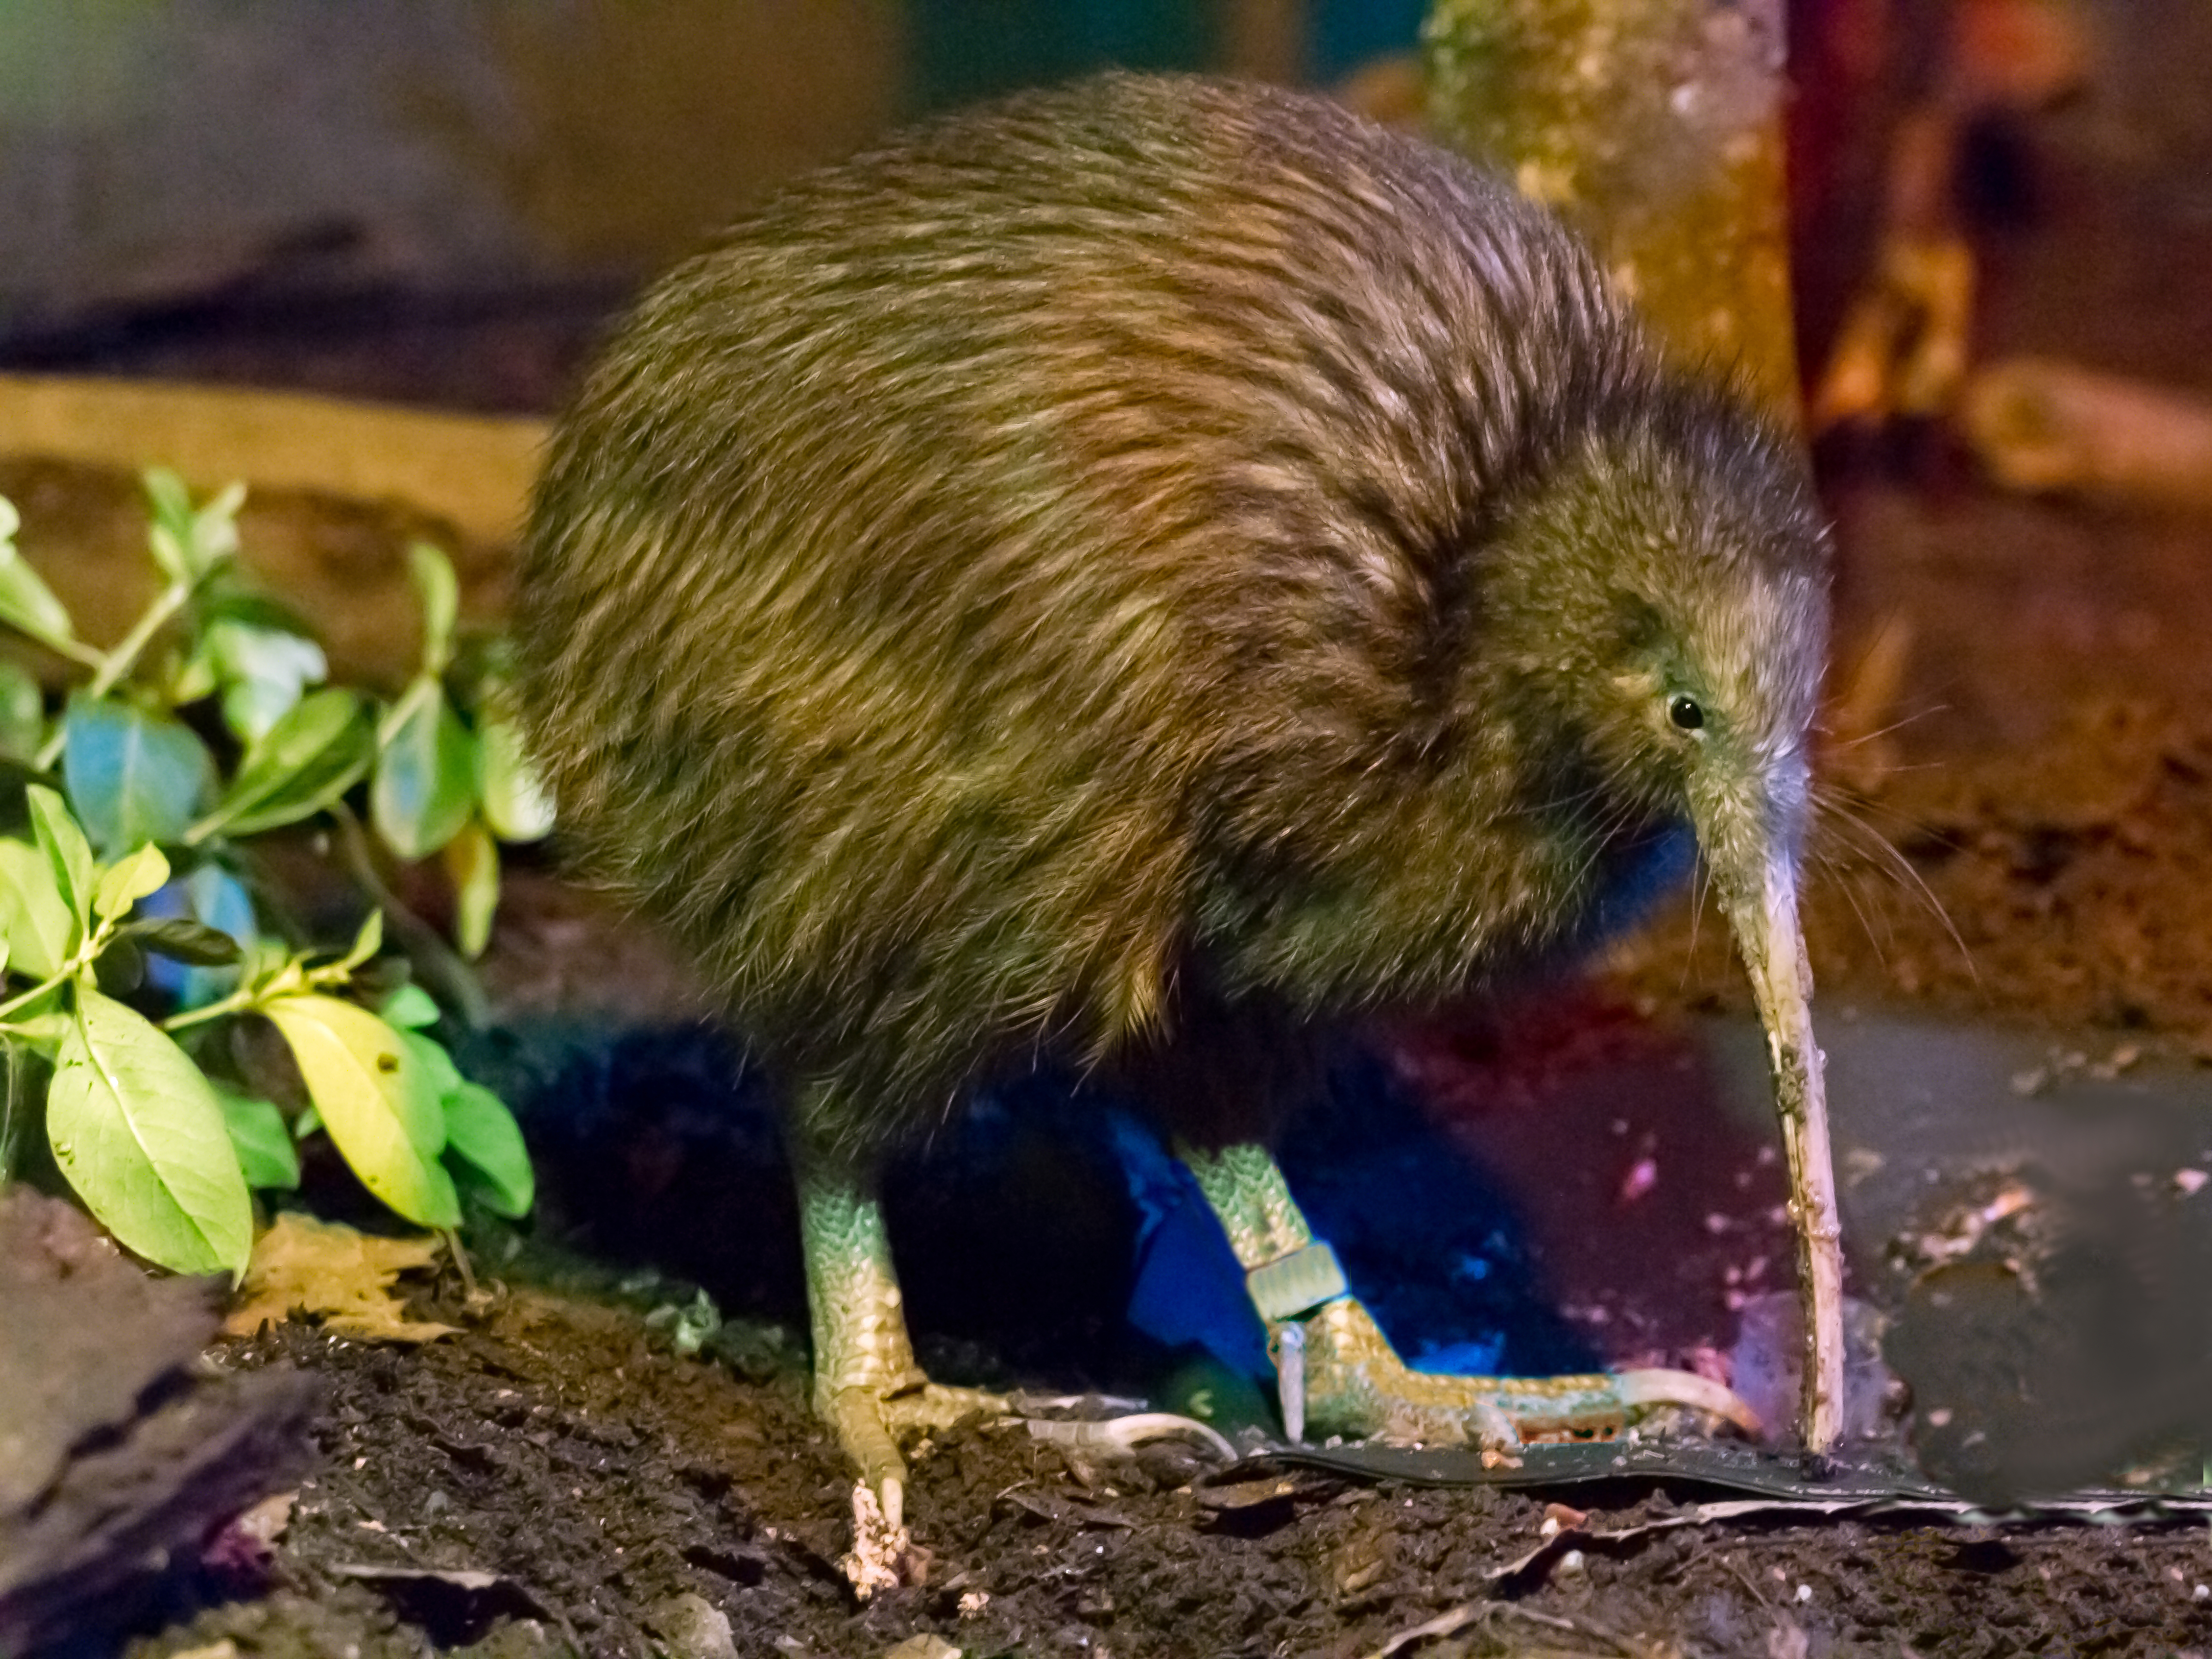
\includegraphics[width=0.1\textwidth]{\GRAPHPATH/kiwi}}}$
  \end{minipage}
\end{frame}

\begin{frame}
  {Programmatisches Schlussbild | Antwort}
  \onslide<+->
  \onslide<+->
  Die ewige Schwachsinnsfrage: Sind Kiwis und Pinguine nun \gruen{Vögel} oder nicht?\\
  \Viertelzeile
  \grau{Nur getoppt von: Erdbeeren sind gar keine Beeren, sondern Sammelnussfrüchte.}\\
  \Zeile
  \begin{itemize}[<+->]
    \item \alert{Kognition} | \orongsch{intrinsisch nicht diskret}, sondern ähnlichkeitsbasiert und \orongsch{parallel}
      \begin{itemize}[<+->]
        \item \orongsch{Netzwerkarchitektur}
      \end{itemize}
      \Halbzeile
    \item \alert{Symbole} = Phone, Morphe, Wörter, Phrasen, \ldots | \orongsch{intrinsisch} diskret und \orongsch{linear}
      \begin{itemize}[<+->]
        \item \orongsch{akustisches} Medium | Sagen Sie mal zwei Wörter gleichzeitig!
        \item \orongsch{schriftliches} Medium | Lesen Sie mal \textit{Zettels Traum}!
      \end{itemize}
    \Halbzeile
    \item[\ding{222}] Da wir nur akustisch oder über schriftliche Artefakte kommunizieren können,\\
      \alert{muss das Sprachsystem symbolisch sein}.
    \item[\ding{222}] Da es architekturbedingt nur nicht-symbolisch verarbeiten kann,\\
      \alert{muss das Gehirn symbolische Systeme so gut wie nötig und möglich emulieren}.
  \end{itemize}
\end{frame}


\begin{frame}
  {Programmatisches Schlussbild | Ausführung}
  \onslide<+->
  \onslide<+->
  Auch nicht-verschriftete Sprache muss medial bedingt logische Eigenschaften haben.\\
  \onslide<+->
  Kulturell bilden sich stärker symbolische Modi aus, vor allem durch Schrift.\\
  \grau{\footnotesize Norm, Selbst- und Fremdkorrektur, Textplanung, intensionale Definitionen, Explizierung, \ldots}\\
  \grau{\footnotesize Warum wird das vor allem im Kontext von Schule, Fremdsprache und Bildungssprache diskutiert?}\\
  \onslide<+->
  \Zeile
  \Halbzeile
  \centering 
  \begin{tabular}[h]{cc}
    \grau{(= spontane Sprachproduktion)} & \\
    \orongsch{weniger symbolische Eigenschaften} & \small \orongsch{informelle Alltagssprache} \\
    \onslide<+->
    \textcolor{orgrA}{\faArrowDown} &\large \textcolor{orgrA}{formelle Alltagssprache} \\
    \onslide<+->
    \textcolor{orgrB}{\faArrowDown} &\Large \textcolor{orgrB}{Bildungssprache} \\
    \onslide<+->
    \textcolor{orgrC}{\faArrowDown} &\LARGE \textcolor{orgrC}{Wissenschaftssprache} \\
    \onslide<+->
    \textcolor{orgrD}{\faArrowDown} &\huge \textcolor{orgrD}{Orthosprache} \\
    \onslide<+->
    \gruen{mehr symbolische Eigenschaften} & \gruen{\Huge formales System} \\
    \grau{(= reflektierte Sprachproduktion)}  & \\
  \end{tabular}
\end{frame}

\begin{frame}
  {Und was ist denn nun mit Kiwis und Pinguinen?}
  \onslide<+->
  \onslide<+->
  Unser Verständnis der Welt führt zu genaueren und diskreten Kategorisierungen,\\
  wo dies nötig ist. \alert{Die Sprache folgt diesem Maß an Genauigkeit und Diskretheit!}\\
  \Zeile
  \onslide<+->
  \centering
  \begin{minipage}{0.9\textwidth}
  \centering
    $\vcenter{\hbox{\includegraphics[height=0.7\textheight]{\GRAPHPATH/birds50}}}$\hspace{0.1\textwidth}
      \only<3>{$\vcenter{\hbox{\rule{0.4\textwidth}{0em}}}$}%
      \only<4>{$\vcenter{\hbox{\includegraphics[width=0.4\textwidth]{\GRAPHPATH/kiwis}}}$}%
      \only<5>{$\vcenter{\hbox{\includegraphics[width=0.4\textwidth]{\GRAPHPATH/penguins}}}$}
  \end{minipage}
\end{frame}

\begin{frame}
  {Letzte Folie}
  \onslide<+->
  \begin{itemize}[<+->]
    \item Viele Missverständnisse in der Linguistik basieren darauf,\\
      dass das eben Gesagte nicht dem allgemeinen Forschungsprogramm zugrundeliegt.
    \item Die Doppelnatur von Sprache führt dazu, dass sowohl rein formale Linguistik\\
      und sogenannte kognitive Linguistik scheinbar erfolgreich sind.
    \item Im Prinzip läuft aber die Linguistik aktuell weitgehend ins Leere.
      \Halbzeile
    \item \alert{Modelltheoretische Semantik beschreibt einen essentiellen Teil von Sprache!}
    \item \alert{Sie modelliert logische Eigenschaften und den Bezug zur realen objektiven Welt.}
      \Halbzeile
    \item \grau{Ganz am Rande zu generativer AI \ldots}
      \begin{itemize}[<+->]
        \item \grau{Erfolg | Sie modelliert völlig natürliche Grammatik.}
        \item \grau{\ldots\ also alle Grammatiker (inkl.\ Chomsky) bitte setzen!}
        \item \grau{Misserfolg | Sie weiß nichts über die Welt,\\
          es wirkt nur so wegen des immensen sprachlichen Inputs.}
        \item \grau{\ldots\ eine Art fancy Papagei.}
      \end{itemize}
  \end{itemize}
\end{frame}

  \let\subsection\section\let\section\woopsi

  \section[Referentielle Semantik]{Referentielle Semantik}
  \let\woopsi\section\let\section\subsection\let\subsection\subsubsection
  \section{Linguistische Theorien}

\begin{frame}
  {Ein neues semiotisches Dreieck}
  \onslide<+->
  \onslide<+->
  Im Sinn der letzten Woche interessiert uns nur die linke Seite.\\
  \onslide<+->
  \Zeile
  \centering 
  \begin{forest}
    [\gruen{Formen}
      [\gruen{Reale Objekte}, edge=gruen]
      [Mentale Konzepte]
    ]
  \end{forest}
\end{frame}

\begin{frame}
  {"`Semantik"' im generativen T-Modell}
  \onslide<+->
  \onslide<+->
  \centering 
  \resizebox{0.6\textwidth}{!}{
    \begin{tikzpicture}

      \node [rectangle, draw, align=left, color=teal, rounded corners=0.5em] (Numeration) at (5cm, -6cm) {Numeration};
      
      \node [visible on=<3->, rectangle, draw, align=left, color=gray] (Lexikon) at (1cm, -6cm) {Lexikon};
      \path (Lexikon.east) edge [visible on=<3->, line width=0.5mm, dashed] node [below, shift={(-0.4cm,0)}] {\textit{}} (Numeration.west);
     
      \node [visible on=<4->, rectangle, draw, align=left, color=gray] (Intention) at (9cm, -6cm) {Intention};
      \path (Intention.west) edge [visible on=<4->, line width=0.5mm, dashed] node [below, shift={(-0.4cm,0)}] {\textit{}} (Numeration.east);

      \node [visible on=<5->, rectangle, draw, align=left, fill=black, color=black, rounded corners=0.5em] (Syntax) at (5cm, -4.5cm) {\whyte{Syntax}};
      \path (Numeration.north) edge [visible on=<5->, line width=0.5mm, -latex] node [below, shift={(-0.4cm,0)}] {\textit{}} (Syntax.south);  

      \node [visible on=<6->, rectangle, draw, align=left, color=teal, rounded corners=0.5em] (Phrasenstruktur) at (5cm, -3cm) {Phrasenstruktur};
      \path (Syntax.north) edge [visible on=<6->, line width=0.5mm, -latex] node [below, shift={(-0.4cm,0)}] {\textit{}} (Phrasenstruktur.south);  

      \node [visible on=<7->, rectangle, draw, align=left, color=teal, rounded corners=0.5em] (PF) at (4cm, 0cm) {PF};
      \path (Phrasenstruktur.north) edge [visible on=<7->, line width=0.5mm, -latex] node [below, shift={(-0.4cm,0)}] {\textit{}} (PF.south);  
     
      \node [visible on=<8->, rectangle, draw, align=left, color=gray] (Aeusserung) at (1cm, 0cm) {Äußerung};
      \path (Aeusserung.east) edge [visible on=<8->, line width=0.5mm, dashed] node [below, shift={(-0.4cm,0)}] {\textit{}} (PF.west);
     
      \node [visible on=<9->, rectangle, draw, align=left, fill=black, color=black, rounded corners=0.5em] (Syntax2) at (6cm, -1.5cm) {\whyte{Syntax 2}};
      \path (Phrasenstruktur.north) edge [visible on=<9->, line width=0.5mm, -latex] node [below, shift={(-0.4cm,0)}] {\textit{}} (Syntax2.south);  
     
      \node [visible on=<10->, rectangle, draw, align=left, color=teal, rounded corners=0.5em] (LF) at (6cm, 0cm) {LF};
      \path (Syntax2.north) edge [visible on=<10->, line width=0.5mm, -latex] node [below, shift={(-0.4cm,0)}] {\textit{}} (LF.south);  

      \node [visible on=<11->, rectangle, draw, align=left, color=gray] (Interpretation) at (9cm, 0cm) {Interpretation};
      \path (Interpretation.west) edge [visible on=<11->, line width=0.5mm, dashed] node [below, shift={(-0.4cm,0)}] {\textit{}} (LF.east);
      
    \end{tikzpicture}
  }
\end{frame}

\begin{frame}
  {Repräsentationsebenen}
  \onslide<+->
  \onslide<+->
  Im klassischen generativen Modell:\\
  \grau{\footnotesize (In minimalistischen Modellen herrscht -- Chomsky muss es mögen! -- sowieso Anarchie.)}
  \Zeile
  \begin{itemize}[<+->]
    \item keine echte Interpretation auf LF
    \item Bewegung \rot{nachdem} der Satz geäußert wurde
    \item Herstellung einer logisch interpretierbaren \alert{Form} auf LF
    \item Grund | Syntax kann nicht alle Interpretationen abbilden
      \Halbzeile
      \begin{itemize}[<+->]
        \item[ ] \alert{Klassiker Quantorenskopus}
        \item[ ] \textit{Everybody loves somebody.}
          \Viertelzeile
        \item[A] Für alle Personen y gilt, dass es eine Person x gibt, für die gilt: y liebt x \grau{($\forall y\exists x.L(y,x)$)}
        \item[B] Es gibt eine Person x, sodass für alle Personen y gilt: y liebt x \grau{($\exists x\forall y.L(y,x)$)}
      \end{itemize}
  \end{itemize}
\end{frame}


\begin{frame}
  {Montagues direkte Interpretation}
  \onslide<+->
  \onslide<+->
  Sprache ist Logik ist Sprache \ldots\\
  \Halbzeile
  \begin{itemize}[<+->]
    \item[A] Entweder ist die \alert{Übersetzung in eine LF trivial und äquivalent zur PF\slash Syntax},\\
      oder \orongsch{sie fügt etwas hinzu, das der Sprache an sich fehlt}.
    \item[B] Sätze haben aber auch \alert{mit LF-Übersetzung nur die Bedeutungen,\\
      die sie sowieso haben} \grau{(keine Hinzufügung)}.
    \item[\ding{222}] Also ist die \gruen{Übersetzung in LF trivial und äquivalent zur PF\slash Syntax}.
    \item[\ding{222}] Wir können \gruen{Sätze direkt interpretieren} (wie sie gesprochen\slash geschrieben werden).
     \Zeile 
   \item \alert{Montagues \textit{lf}} | direkte Übersetzung von sprachlichen in logische Ausdrücke
  \end{itemize}
\end{frame}

\section{Referentielle Semantik basal}

\begin{frame}
  {Interessante Eigenschaften von Sprache}
  \onslide<+->
  \begin{itemize}[<+->]
    \item Aussagen über die\slash Teile der Welt
    \item Ausdrücke bezeichnen\slash referieren auf Dinge i.\,w.\,S.
    \item Informativität
    \item objektiv beurteilbar (\zB Wahrheit von Sätzen)
      \Zeile
    \item \alert{Aber welche sprachlichen Einheiten referieren auf was?}
  \end{itemize}
\end{frame}

\begin{frame}
  {Referenz | Eigennamen}
  \onslide<+->
  \onslide<+->
  Ein \alert{Eigenname} \ding{222} \alert{genau ein Objekt} in der Welt\\
  \onslide<+->
  \Zeile
  \centering
    \begin{tikzpicture}
      \node [] (name) at (-6cm, 0cm) {\textit{Jan Böhmermann}};
      \node [visible on=<4->] (boehmi) at (0cm, 0cm) {\includegraphics[width=0.2\textwidth]{\GRAPHPATH/boehmermann}};
      \path (name.east) edge [visible on=<4->, line width=0.5mm, -latex] node {\textit{}} (boehmi.west);
    \end{tikzpicture}
\end{frame}

\begin{frame}
  {Referenz | Appellativa}
  \onslide<+->
  \onslide<+->
  Ein normales \alert{Nomen} \ding{222} \alert{eine Menge von Objekten} in der Welt\\
  \onslide<+->
  \Zeile
  \centering
    \begin{tikzpicture}
      \node [] (noun) at (-6cm, 0cm) {\textit{soldier}};
      \node [visible on=<4->] (soldiers) at (0cm, 0cm) {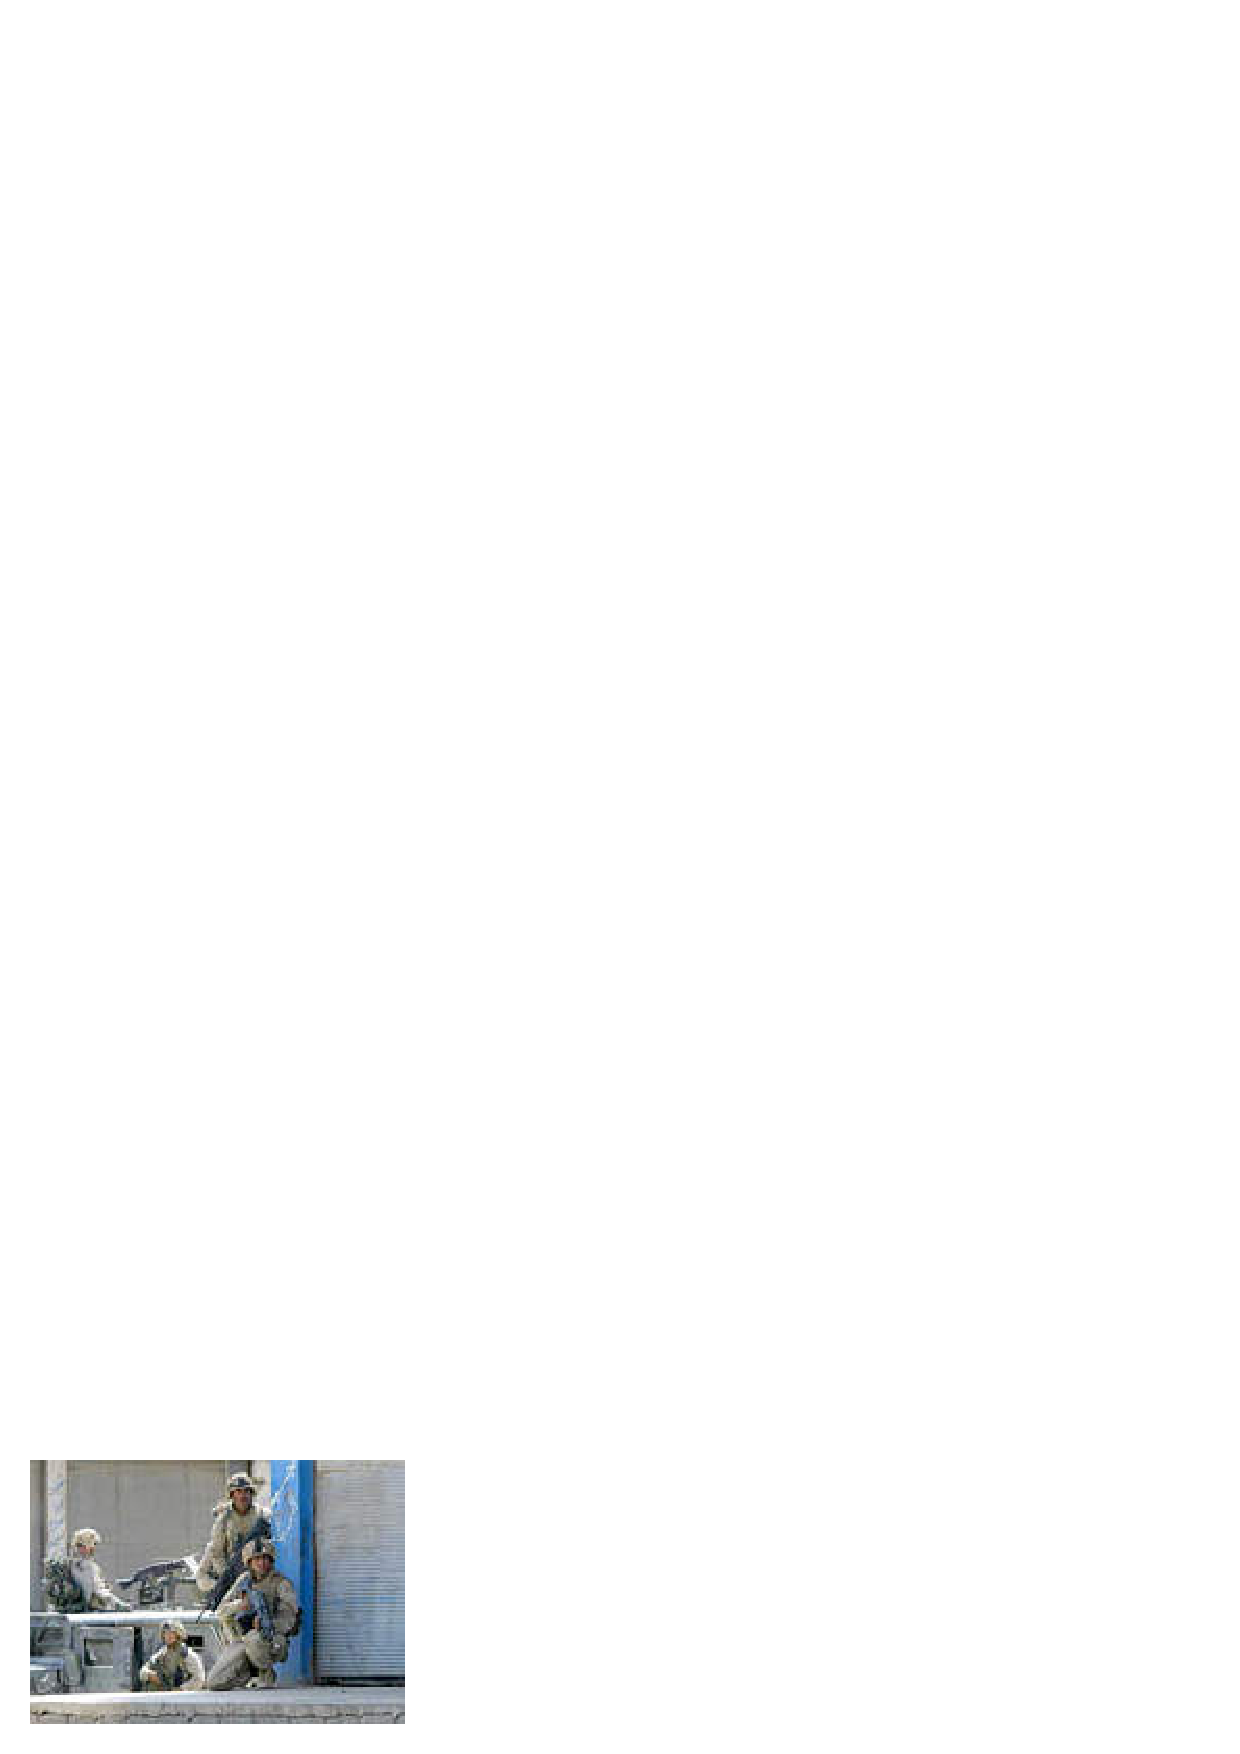
\includegraphics[width=0.2\textwidth]{\GRAPHPATH/soldiers}};
      \path (noun.east) edge [visible on=<4->, line width=0.5mm, -latex] node {\textit{}} (soldiers.west);
    \end{tikzpicture}
\end{frame}

\begin{frame}
  {Referenz | Adjektive und Verben}
  \onslide<+->
  \onslide<+->
  Ein (intersektives) \alert{Adjektiv} oder ein \alert{Verb} \ding{222} \alert{eine Menge von Objekten} in der Welt\\
  \onslide<+->
  \Zeile
  \centering
    \begin{tikzpicture}
      \node [] (adj) at (-6cm, 0cm) {\textit{human}};
      \node [visible on=<4->] (boehmi) at (0cm, +2cm) {\includegraphics[width=0.1\textwidth]{\GRAPHPATH/boehmermann}};
      \path (adj.east) edge [visible on=<4->, line width=0.5mm, -latex] node {\textit{}} (boehmi.west);
      \node [visible on=<5->] (soldiers) at (0cm, 0cm) {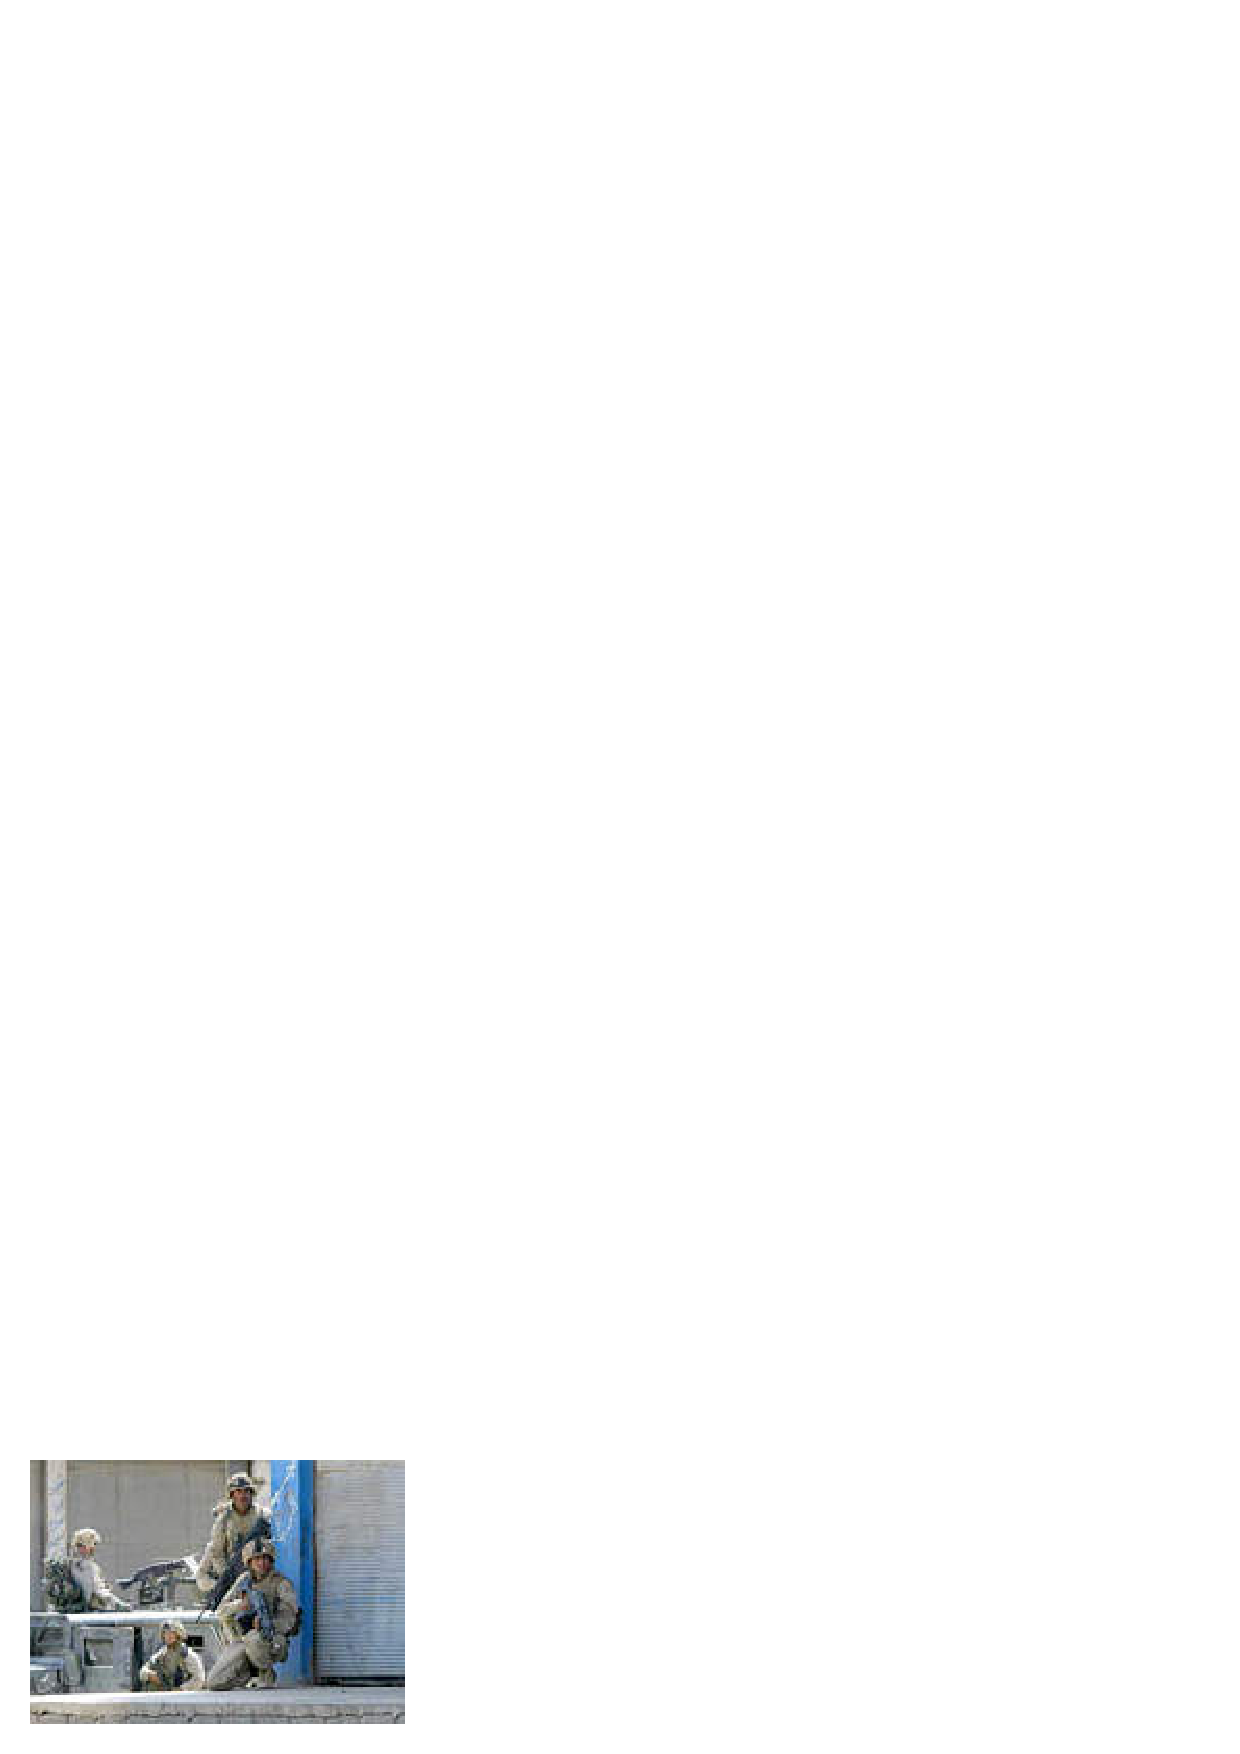
\includegraphics[width=0.1\textwidth]{\GRAPHPATH/soldiers}};
      \path (adj.east) edge [visible on=<5->, line width=0.5mm, -latex] node {\textit{}} (soldiers.west);
      \node [visible on=<6->] (crowd) at (0cm, -2cm) {\includegraphics[width=0.1\textwidth]{\GRAPHPATH/crowd}};
      \path (adj.east) edge [visible on=<6->, line width=0.5mm, -latex] node {\textit{}} (crowd.west);
    \end{tikzpicture}
\end{frame}

\begin{frame}
  {Referenz | Sätze}
  \onslide<+->
  \onslide<+->
  Ein \alert{Satz} \ding{222} in erster Näherung \alert{ein Sachverhalt}\\
  \onslide<+->
  \Zeile
  \centering
    \begin{tikzpicture}
      \node [align=left] (s) at (-6cm, 0cm) {\it A humming bird\\\it is hovering over\\\it a red flower.};

      \node [visible on=<4->, align=center] (hum) at (0cm, +2cm) {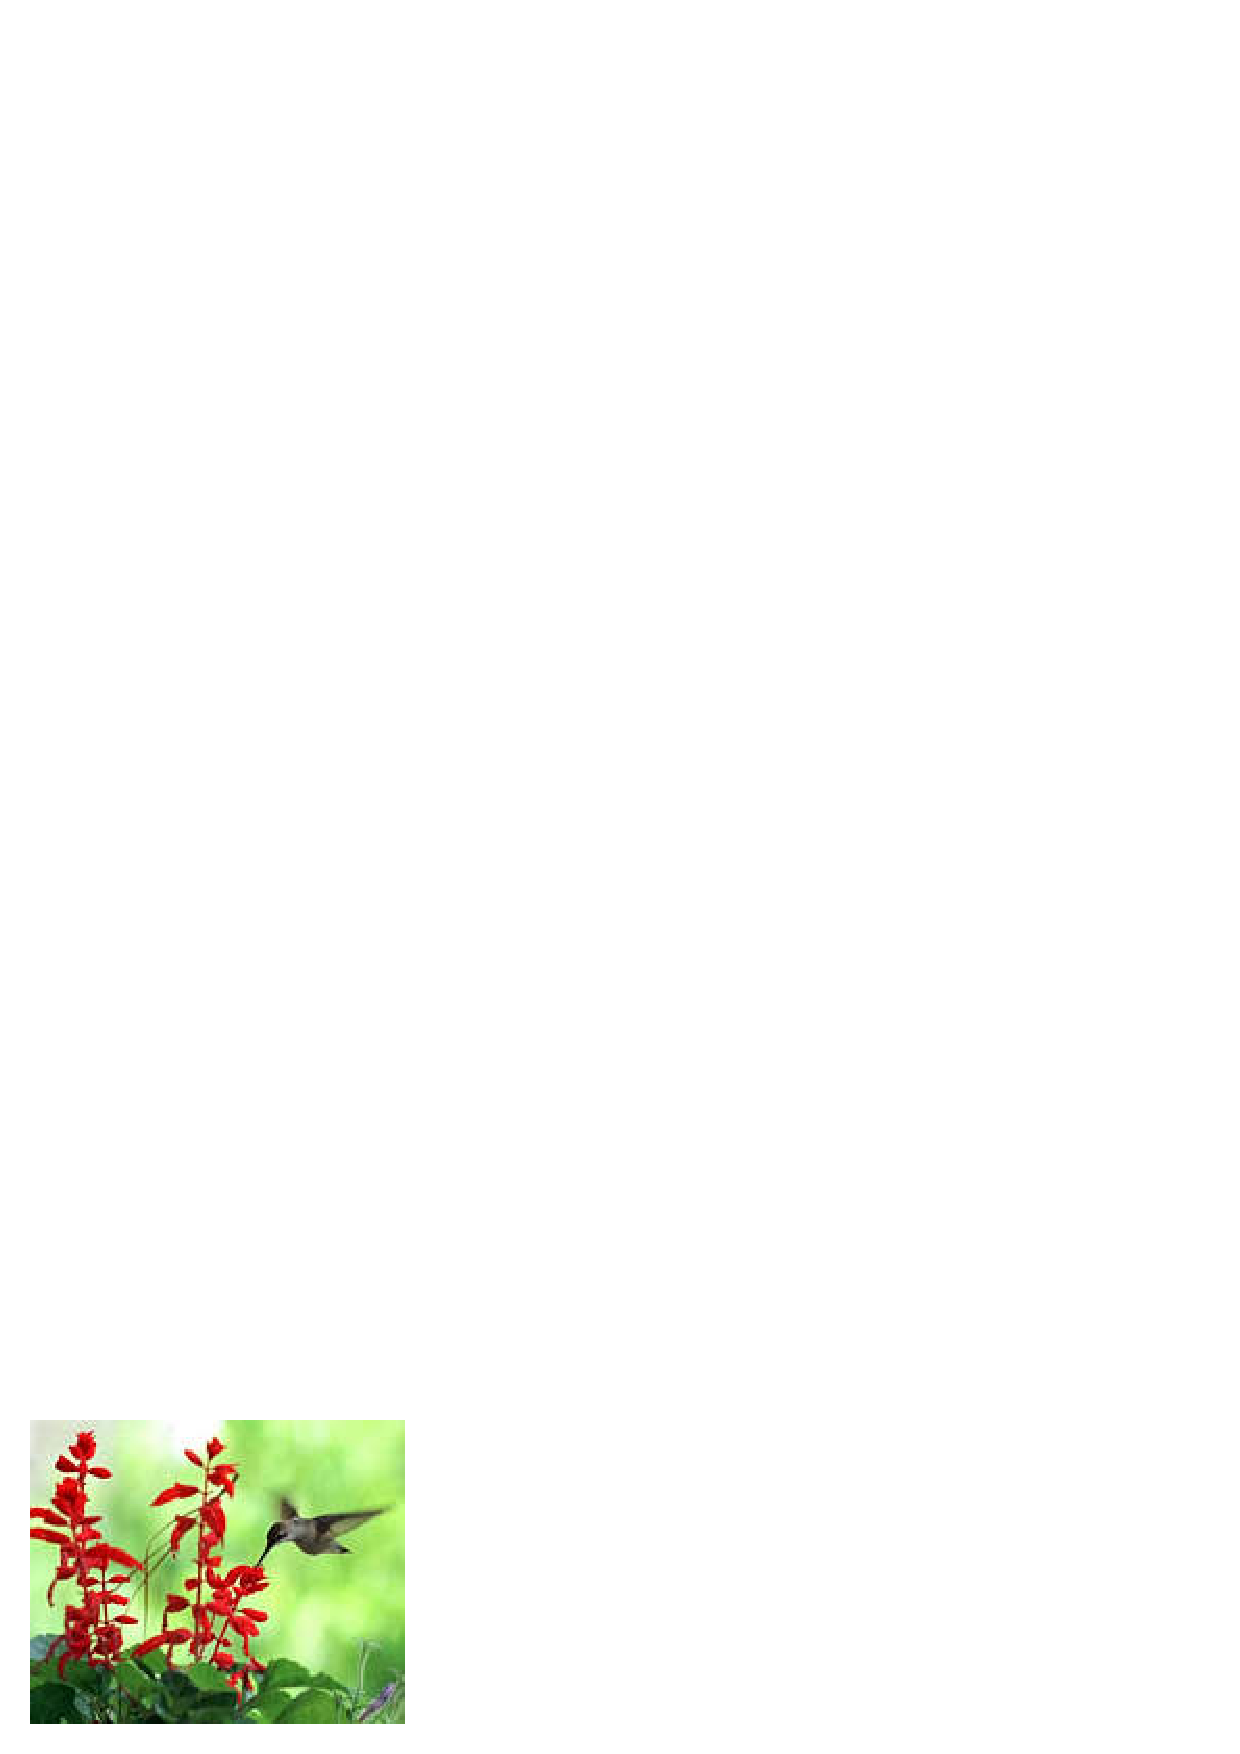
\includegraphics[width=0.2\textwidth]{\GRAPHPATH/hummingbird}};
      \path (s.east) edge [visible on=<4->, line width=0.5mm, -latex] node {\textit{}} (hum.west);
      
      \node [visible on=<5->, align=center] (boehmi) at (0cm, -2cm) {\includegraphics[width=0.2\textwidth]{\GRAPHPATH/boehmermann}\\\footnotesize (als Individuum)};
      \path (s.east) edge [visible on=<5->, line width=0.5mm, -latex, color=red] node {\textit{}} (boehmi.west);
      \node [visible on=<6->, align=center, color=red, fill=red] (nein) at (-3.5cm, -1.25cm) {\footnotesize \whyte{Nein! falsche}\\\footnotesize \whyte{Art von Objekt}};
    \end{tikzpicture}
\end{frame}

\begin{frame}
  {Freges Prinzip | Das hier wollen wir formalisieren!}
  \onslide<+->
  \onslide<+->
  Bedeutung ist kompositional!\\
  \Halbzeile
  \begin{itemize}[<+->]\small
    \item \textit{humming bird} \ding{222} die \alert{Menge} der Kolibri-Objekte
    \item \textit{a} \ding{222} \alert{Existenzaussage} für ein Element aus einer Menge
    \item \textit{a humming bird} \ding{222} \alert{Existenzaussage} für ein Element $x$\\
      aus der Menge der Kolibri-Objekte
    \item \textit{is hovering} \ding{222} die \alert{Menge} der schwebenden Objekten
    \item \textit{a humming bird is hovering} \ding{222} das existierende Kolibri-Objekt $x$\\
      ist auch ein \alert{Element der Menge} der schwebenden Objekte
    \item \textit{a red flower} \ding{222} \alert{Existenzaussage} für ein Element $y$\\
      aus der \alert{Schnittmenge} der roten Objekte und der Blumen-Objekte
    \item \textit{over} \ding{222} die \alert{Relation} zwischen Objekten (s.\ nächste Woche),\\
      die sich übereinander befinden
    \item \textit{A Humming is hovering over a red flower.} \ding{222}\\
      \gruen{Es gibt ein Objekt $x$ aus der Schnittmenge der Kolibri- und der schwebenden Objekte,\\
      und es gibt ein Objekt $y$ aus der Schnittmenge der roten und der Blumen-Objekte,\\
    und $x$ befindet sich über $y$.}
  \end{itemize}
\end{frame}

\section{Semantische Eigenschaften von Sätzen}

\begin{frame}
  {Implikation (Entailment)}
  \onslide<+->
  \onslide<+->
  Mengen von Aussagesätzen \alert{implizieren} andere Sätze.\\
  \onslide<+->
  Sätze (Implikationen) lassen sich aus anderen Sätzen (Axiome) \alert{beweisen}.\\
  \Halbzeile
  \begin{itemize}[<+->]
    \item[A] \textit{Jan Böhmermann ist ein Mensch.}
    \item[B] \textit{Jan Böhmermann ist leutselig.}
    \item[C] \textit{Jan Böhmermann ist ein leutseliger Mensch.}
      \Halbzeile
    \item[ ] \alert{$A,B\vdash C$} | A und B implizieren C. (C ist beweisbar aus A und B.)
    \item[ ] \rot{$A\not\vdash C$} | A impliziert nicht C.
    \item[ ] \rot{$B\not\vdash C$} | B impliziert nicht C.
      \Halbzeile
    \item[ ] \orongsch{$A\vdash A\wedge A$} \onslide<+->| \textit{Jan Böhmermann ist ein Mensch \orongsch{und} Jan Böhmermann ist ein Mensch.}
      \Halbzeile
    \item[D] \textit{Irgendetwas ist ein Mensch.}
    \item[ ] \alert{$A\vdash D$} 
  \end{itemize}
\end{frame}

\begin{frame}
  {Tests auf Implikation}
  \onslide<+->
  \onslide<+->
  Wenn diese Kriterien zutreffen, impliziert A B:\\
  \Zeile
  \begin{itemize}[<+->]
    \item Wenn A wahr ist, ist B auch immer wahr.
    \item Eine Situation, die von B beschrieben wird, wird auch von A beschrieben.
    \item Die Information in B ist vollständig in der Information in A enthalten.
    \item Man kann unter keinen Umständen sagen: \textit{A ist wahr, aber B ist nicht wahr.}
  \end{itemize}
\end{frame}

\begin{frame}
  {Übung | Sind das Implikationen?}
  \begin{itemize}[<+->]\small
    \item Böhmermann ist Showmaster. $\vdash$ Böhmermann ist menschlich.
    \item Böhmermann ist nicht sehr groß. $\vdash$ Irgendjemand ist nicht sehr groß.
    \item Böhmermann ist nicht sehr groß. $\vdash$ Irgendjemand ist sehr groß.
    \item Manche Menschen sind leutselig. $\vdash$ Böhmermann ist leutselig.
    \item Ich habe das neue drip-133-Album gehört. $\vdash$ drip-133 hat ein neues Album veröffentlicht.
    \item Nachdem ich einen Sherry getrunken habe, habe ich den Kondensator getauscht.\\
      $\vdash$ Ich habe einen Sherry getrunken.
    \item Nachdem Linux nicht mehr startete, habe ich einen weiteren Sherry getrunken.\\
      $\vdash$ Linux ist noch nie gestartet.
    \item Mein ehemaliger Mitbewohner mag Becks.\\
      $\vdash$ Mein ehemaliger Mitbewohner könnte Sherry mögen.
    \item Böhmermann hat das heutige ZDF Magazin beendet.\\
      $\vdash$ Das heutige ZDF Magazin wurde beendet.
  \end{itemize}
\end{frame}

\begin{frame}
  {Präsupposition | Der anzunehmende Hintergrund}
  \onslide<+->
  \onslide<+->
  Präsuppositionen sind schwächer als Implikationen.\\
  \Zeile
  \begin{itemize}[<+->]
    \item[A] \textit{Willy Brandt ist der gegenwärtige Kanzler Deutschlands.}
    \item[B] \textit{Wenn Willy Brandt der gegenwärtige Kanzler Deutschlands ist,\\
      trägt er eine große Verantwortung.}
    \item[C] \textit{Willy Brandt ist nicht der gegenwärtige Kanzler Deutschlands.}
    \item[D] \textit{Willy Brandt lebt.}
    \item[E] \textit{Es gibt einen Kanzler Deutschlands.}
      \Halbzeile
    \item \alert{A und B präsupponieren D.} = D ist eine Voraussetzung\\
      für eine erfolgreiche Interpretation von A und B.
    \item \orongsch{C präsupponiert nicht D.}
    \item \alert{A, B und C präsupponieren E.}
  \end{itemize}
\end{frame}

\begin{frame}
  {Tests auf Präsupposition}
  \onslide<+->
  \onslide<+->
  Die Unterschiede zur Implikation sind relevant.\\
  \Halbzeile
  \begin{itemize}[<+->]
    \item Nicht nur Aussagesätzen haben Präsuppositionen (Modale, Konditionale, \ldots)
    \item Negierte Sätze haben oft gleiche Präsuppositionen wie nicht-negierte.
    \item Präsuppositionen können negiert werden, und der Ausgangssatz bleibt wahr.\\
      \grau{(Geht nicht mit Implikationen.)}
      \begin{itemize}[<+->]
        \item[F] \textit{Willy Brandt ist nicht Kanzler Deutschlands.}
        \item[G] \textit{Es gibt einen Kanzler Deutschlands.}
        \item[ ] F präsupponiert G, bleibt aber wahr, wenn G falsch ist.
      \end{itemize}
  \end{itemize}
\end{frame}

\begin{frame}
  {Synonymie}
  \onslide<+->
  \onslide<+->
  Synonyme Ausdrücke haben \orongsch{exakt} \alert{die gleiche Referenz}.\\
  \Halbzeile
  \begin{itemize}[<+->]
    \item lexikalische Synonymie | \textit{humming bird} $\stackrel{lex}{\equiv}$ \textit{colibri}
      \Halbzeile
    \item kompositionale Synonymie
      \begin{itemize}[<+->]
        \item[ ] \textit{Mulder traf seine entführte Schwester, nachdem er\\
          in die geheime Militärbasis eingebrochen war.}
        \item[$\equiv$] \textit{Bevor er seine entführte Schwester traf,\\
          brach Mulder in die geheime Militärbasis ein.}
      \end{itemize}
    \Halbzeile
    \item \alert{$A\equiv B\ \text{gdw}\ A\vdash B\ \text{und}\ B\vdash A$} (gegenseitige Implikation)
    \item \grau{\textit{gdw} = \textit{genau dann wenn} | \textit{iff} = \textit{if and only if}}
  \end{itemize}
\end{frame}

\section{Referenz von Sätzen}

\begin{frame}
  {Natürliche Sprache und Implikation}
  \onslide<+->
  \onslide<+->
  Referentielle Semantik $\not=$ \alert{\textit{einfaches Zeigen auf Objekte durch Sprache}}.\\
  \Viertelzeile
  \onslide<+->
  Zusätzliche Logik für Fälle wie diesen (und viele andere):\\
  \Zeile
  \onslide<+->
  \begin{tabular}[h]{lll}
    & \alert{\textit{Die Lieblingsblume meines Kolibris}} & \textit{ist rot.} \\
    \visible<6->{\orongsch{$\vdash$}} & \visible<5->{\alert{\textit{Eine Blume}} & \textit{ist rot.}} \\
  \end{tabular}
\end{frame}

\begin{frame}
  {Sätze referieren aus Wahrheitswerte!}
  \onslide<+->
  \onslide<+->
  \centering 
  Um zu der gewünschten Logik zu kommen, zeigen wir jetzt,\\
  dass \alert{Sätze auf Wahrheitswerte referieren}.\\
  \Halbzeile
  \onslide<+->
  Wahrheitswerte sind nur \alert{\textit{wahr}} und \alert{\textit{falsch}}.\\
  \Halbzeile
  \onslide<+->
  Die Verben \alert{\textit{denotieren}} und \textit{\alert{referieren auf}} sind hier synonym.\\
  \Doppelzeile
  \onslide<+->
  Warten Sie bitte ein paar Wochen, wenn Sie diese Darstellung reduktionistisch finden.
\end{frame}

\begin{frame}
  {Synonyme NPs}
  \onslide<+->
  \begin{itemize}[<+->]
    \item[a] \textit{colibri}
    \item[b] \textit{humming bird}
    \item[ ] \gruen{$a\stackrel{lex}{\equiv} b$}
      \Halbzeile
    \item[c] \textit{a brunette lady}
    \item[d] \textit{a brown-haired dame}
    \item[ ] \gruen{$c\equiv d$}
      \Halbzeile
    \item[e] \textit{the primates}
    \item[f] \textit{the apes and humans}
    \item[ ] \gruen{$e\equiv f$}
  \end{itemize}
\end{frame}

\begin{frame}
  {Synonymie von Konstituenten und Sätzen}
  Synonymie von Konstituenten im Satzkontext \ding{222} Satzsynonymie\\
  \onslide<+->
  \Halbzeile
  \begin{itemize}[<+->]
    \item[A] \alert{\textit{A \orongsch{colibri} is hovering over a red flower.}}
    \item[B] \alert{\textit{A \orongsch{humming bird} is hovering over a red flower.}}
    \item[ ] \gruen{$A\equiv B$ weil $a\equiv b$ und Satzkontext identisch}
    \item[ ] \gruen{$[\Sub{A} a]\equiv[\Sub{B} b]$ wenn $a\equiv b$ und $[\Sub{A} \_]=[\Sub{B} \_]$}
      \Halbzeile
    \item[C] \alert{\textit{Lauren Bacall was \orongsch{a brunette lady}.}}
    \item[D] \alert{\textit{Lauren Bacall was \orongsch{a brown-haired dame}.}}
    \item[ ] \gruen{$C\equiv D$ weil $c\equiv d$ und Satzkontext identisch}
      \Halbzeile
    \item[E] \alert{\textit{\orongsch{Primates} are intelligent.}}
    \item[F] \alert{\textit{\orongsch{The apes and humans} are intelligent.}}
    \item[ ] \gruen{$E\equiv F$ weil $e\equiv f$ und Satzkontext identisch}
  \end{itemize}
\end{frame}

\begin{frame}
  {Zwei Axiome}
  \onslide<+->
  \begin{itemize}[<+->]
    \item[ ] Referenz\slash Denotat eines Ausdrucks A als \alert{\den{A}}\\
      \grau{$\dem{\cdot}$ ist eine Funktion!}
      \Zeile
    \item[ ] Erinnerung: Synonymität von Sätzen ist gegenseitige Implikation.
      \Zeile
    \item[Ax1] Synonyme Ausdrücke (NPs, Verben, Sätze, \ldots) haben dieselbe Referenz.
    \item[ ] Formal: \alert{$A\equiv B\leftrightarrow\den{A}=\den{B}$}
      \Zeile
    \item[Ax2] Wenn wir in Ausdruck C einen Ausdruck A durch\\
      einen synonymen Ausdruck B ersetzen, behält C seine Referenz.
    \item[ ] Formal: \alert{$\den{A}=\den{B}\rightarrow\den{[\Sub{C} A]}=\den{[\Sub{C} B]}$}
  \end{itemize}
\end{frame}

\begin{frame}
  {Zwei wahre Sätze}
  \onslide<+->
  \onslide<+->
  Wahrheitswert von A und B | \alert{1} bzw.\ \alert{\textit{wahr}} bzw.\ \alert{\textit{true}} oder \alert{\textit{T}}\\
  \Zeile
  \begin{itemize}[<+->]
    \item[A] \textit{Lauren Bacall was a brunette lady.}
    \item[B] \textit{My humming bird's favourite flower is red.} 
  \end{itemize}
\end{frame}

\begin{frame}
  {Erste Schlussfolgerung}
  \onslide<+->
  \onslide<+->
  Einsetzen von A und B in \alert{Satzkontext T bzw. $[\Sub{T}\_]$} (Aussage über Wahrheitswert)\\
  \Halbzeile
  \begin{itemize}[<+->]
    \item[T] \alert{\textit{The truth value of `\_' is 1.}}
      \Halbzeile
    \item[{[\Sub{T}A]}] \alert{\textit{The truth value of `\orongsch{Lauren Bacall was a brunette lady.}' is 1.}}
    \item[{[\Sub{T}B]}] \alert{\textit{The truth value of `\orongsch{My humming bird's favourite flower is red.}' is 1.}}
      \Halbzeile
    \item[ ] folgt \gruen{$A\equiv[\Sub{T}A]$} und \gruen{$B\equiv[\Sub{T}B]$}
    \item[ ] mit Ax1 \gruen{$\den{A}=\den{[\Sub{T}A]}$} und \gruen{$\den{B}=\den{[\Sub{T}B]}$}
      \Halbzeile
    \item[ ] Bitte bedenken: $A$ und $[\Sub{T}A]$ haben auch intuitiv "`denselben Inhalt"'.
  \end{itemize}
\end{frame}

\begin{frame}
  {Zweite Schlussforlgerung}
  \onslide<+->
  \onslide<+->
  In $[\Sub{T}A]$ und $[\Sub{T}B]$ sind A und B jeweils in einer NP eingebettet.\\
  \Halbzeile
  \begin{itemize}[<+->]
    \item $\den{the truth value of A}=\den{the truth value of B}=1$
    \item[ ] mit Ax2 \gruen{$\den{[\Sub{T}A]}=\den{[\Sub{T}B]}$}
    \item[ ] damit \gruen{$\den{A}=\den{[\Sub{T}A]}=\den{[\Sub{T}B]}=\den{B}=1$}
      \Halbzeile
    \item \gruen{Sätze referieren auf Wahrheitswerte.}\\
      \grau{(Denn man kann das mit zwei beliebigen wahren Sätzen machen.)}
    \item Achtung | \gruen{Wahrheitswerte sind auch nur realweltliche Objekte.}
  \end{itemize}
\end{frame}

\begin{frame}
  {Adäquatheit von Wahrheitswerten als Satzreferenten}
  \onslide<+->
  \onslide<+->
  Nicht so \rot{sinnlos}, \rot{schwachsinnig}, \rot{inhaltsleer}, \ldots\ wie oft vermutet\\
  \Zeile
  \begin{itemize}[<+->]
    \item Referentielle Semantik
      \begin{itemize}[<+->]
        \item Analyse der Referenten verschiedener Typen von Ausdrücken
        \item Komposition von Sätzen
        \item deduktive Logik für Sätze
        \item \alert{Benennen der Wahrheitsbedingungen} (\ding{222} Modelltheorie)
      \end{itemize}
      \Halbzeile
    \item minimale Gemeinsamkeit \alert{aller} Sätze
    \item gut formal berechenbar (Binarität)
    \item reichhaltigere Semantik später (basierend auf Wahrheitswerten)
  \end{itemize}
\end{frame}

\section{Reden in Fragmenten}

\begin{frame}
  {Grammatik- und Semantikfragmente}
  \onslide<+->
  \onslide<+->
  \alert{Konstruktive}, \alert{schrittweise} Annäherungen an sprachliche Modellierung\\
  \Zeile
  \begin{itemize}[<+->]
    \item Grammatikfragment | Ausschnitt einer Gesamtgrammatik
    \item erwünschte schrittweise Erweiterung von Fragmenten (vgl.\ HPSG)
      \Zeile
    \item Konstruktion eines Semantik-Fragments
      \begin{itemize}[<+->]
         \item grammatische Kategorien und Referenzen von Wörtern
         \item Grammatikmechanismen und zugehörige Bedeutungskonstruktion
         \item Ergebnis | Semantik von Sätzen und Beitrag aller Konstituenten dazu
      \end{itemize}
    \item \Halbzeile
      \alert{T-Sätze}
      \begin{itemize}[<+->]
        \item \alert{L} eine Sprache, \alert{S} ein Satz, \alert{v} ein Sachverhalt, \alert{p} eine Aussage über Wahrheitsbedingungen
        \item \alert{S aus L ist wahr in v gdw p.}
      \end{itemize}
  \end{itemize}
\end{frame}

\begin{frame}
  {Das Lexikon}
  \onslide<+->
  \onslide<+->
  Die folgenden simplexen Ausdrücke sind Teil von F\Sub{1}.\\
  \onslide<+->
  Kein anderer simplexer Ausdruck ist Teil von F\Sub{1}.\\
  \Halbzeile
  \begin{enumerate}[<+->]
    \item N $\rightarrow$ \emph{Herr Webelhuth, Frau Klenk, the Turm-Mensa} \label{lex01}
    \item V\Sub{{i}} $\rightarrow$ \emph{is relaxed, is creative, is stupid} \label{lex02}
    \item V\Sub{t} $\rightarrow$ \emph{prefers} \label{lex03}
    \item conj $\rightarrow$ \emph{and, or} \label{lex04}
    \item neg $\rightarrow$ \emph{it is not the case that} \label{lex05}
  \end{enumerate}
\end{frame}

\begin{frame}
  {Die Phrasenstrukturgrammatik von F\Sub{1}}
  \onslide<+->
  \onslide<+->
  Folgende Kompositionsregeln sind Teil von F\Sub{1}.\\
  Keine andere Kompositionsregel ist Teil von F\Sub{1}.\\
  \Halbzeile
  \begin{enumerate}[<+->]
    \item S $\rightarrow$ N VP \label{syn01}
    \item S $\rightarrow$ S conj S \label{syn02}
    \item S $\rightarrow$ neg S \label{syn03}
    \item VP $\rightarrow$ V\Sub{{i}} \label{syn04}
    \item VP $\rightarrow$ V\Sub{t} N \label{syn05}
  \end{enumerate}
\end{frame}

\begin{frame}
  {Referenz simplexer Ausdrücke}
  \begin{itemize}[<+->]
    \item $\llbracket$Herr Webelhuth$\rrbracket$ = Herr Webelhuth \label{lexint01}
    \item $\llbracket$Frau Klenk$\rrbracket$ = Frau Klenk \label{lexint02}
    \item $\llbracket$the Turm-Mensa$\rrbracket$ = the Turm-Mensa \label{lexint03}
    \item $\llbracket$is relaxed$\rrbracket$ = \{x:x is relaxed\} \label{lexint04}
    \item $\llbracket$is creative$\rrbracket$ = \{x:x is creative\} \label{lexint05}
    \item $\llbracket$is stupid$\rrbracket$ = \{x:x is stupid\} \label{lexint06}
    \item $\llbracket$prefers$\rrbracket$ = \{$\langle$x,y$\rangle$: x prefers y\} \label{lexint07}
  \end{itemize}
\end{frame}

\begin{frame}
  {Referenz von Funktionswörtern}
  Funktionswörter referieren auf \alert{Funktionen}.\\
  \Zeile
  \begin{itemize}[<+->]
    \item $\dem{neg} = \left[
                       \begin{array}{l}
                                1 \rightarrow 0\\
                                0 \rightarrow 1
                       \end{array}
                     \right]$ \label{fint01}
    \item $\dem{and} = \left[
                       \begin{array}{l}
                                \langle 1,1 \rangle \rightarrow 1\\
                                \langle 1,0 \rangle \rightarrow 0\\
                                \langle 0,1 \rangle \rightarrow 0\\
                                \langle 0,0 \rangle \rightarrow 0
                       \end{array}
                       \right]$ \label{fint02}
    \item $\dem{or} = \left[
                           \begin{array}{l}
                                    \langle 1,1 \rangle \rightarrow 1\\
                                    \langle 1,0 \rangle \rightarrow 1\\
                                    \langle 0,1 \rangle \rightarrow 1\\
                                    \langle 0,0 \rangle \rightarrow 0
                           \end{array}
                           \right]$ \label{fint03}
  \end{itemize}
\end{frame}

\begin{frame}
  {T-Sätze für F\Sub{1}}
  \begin{itemize}[<+->]
    \item \den{\alert{[\Sub{S}{ }N{ }VP]}} = 1 iff \den{N} $\in$ \den{VP}, else 0 \label{t01}
    \item \den{\alert{[\Sub{S} S1 conj S2]}} = \den{conj} ($\langle$\den{S1},\den{S2}$\rangle$) \label{t02}
    \item \den{\alert{[\Sub{S} neg S]}} = \den{neg} (\den{S}) \label{t03}
    \item \den{\alert{[\Sub{VP} V\Sub{t} N]}} = \{x: $\langle$x, \den{N} $\rangle$ $\in$ \den{V\Sub{t}}\} \label{t04}
      \Halbzeile
    \item für einen nicht verzweigenden Knoten K und seine Tochter D: $\dem{[\Sub{K} D]}=\dem{D}$ \label{t05}
      \Halbzeile
    \item \grau{Das geht alles eleganter. Bitte etwas Geduld!}
  \end{itemize}
\end{frame}

\begin{frame}
  {Schritt 1 | Syntax parsen}
  Ist folgendes ein Satz aus F\Sub{1}? \onslide<+-> \alert{\textit{Herr Webelhuth is relaxed.}}\\
  \Halbzeile
  \begin{itemize}[<+->]
    \item{} [\Sub{N} \textit{Herr Webelhuth}] mit \gruen{Lexikonregel \ref{lex01}}
    \item{} [\Sub{V\Sub{i}} \textit{is relaxed}] mit \gruen{Lexikonregel \ref{lex02}}
    \item{} [\Sub{VP} [\Sub{V\Sub{i}} \textit{is relaxed}]] mit \gruen{Syntaxregel \ref{syn04}}
    \item{} [\Sub{S} [\Sub{N} \textit{Herr Webelhuth}] \Sub{VP} [\Sub{V\Sub{i}} \textit{is relaxed}]] mit \gruen{Syntax \ref{syn01}}
  \end{itemize}
\end{frame}

\begin{frame}
  {Syntax als Baum}
  \centering 
  \begin{forest}
    [S
      [N
        [\textit{Herr Webelhuth}]
      ]
      [VP
        [V\Sub{i}
          [\textit{is relaxed}]
        ]
      ]
    ]
  \end{forest}
\end{frame}

\begin{frame}
  {Semantik | Referenz der Teile und ihrer Bedeutung}
  \onslide<+->
  \onslide<+->
  \alert{v} (Sachverhalt) | Herr Webelhuth (das ontologische Objekt) $\in$\{x: x is relaxed\}\\
  \Halbzeile
  \begin{itemize}[<+->]
    \item für N: \den{\textit{Herr Webelhuth}} = Herr Webelhuth (das ontologische Objekt)
    \item für VP (und V\Sub{i}): \den{\textit{is relaxed}} = \{x: x is relaxed\} (enthält Herrn Webelhuth)
    \item für S: \den{[\Sub{S}{ }N{ }VP]} = 1 iff \den{N} $\in$ \den{VP}, else 0
      \Halbzeile
    \item in v daher \gruen{\den{[\Sub{S} \textit{Herr Webelhuth is relaxed.}]}=1}
  \end{itemize}
\end{frame}

\begin{frame}
  {Semantik als Baum}
  \begin{tabular}[h]{cc}
  \onslide<+->
  \onslide<+->
  \centering 
  \begin{forest}
    [\den{S}
      [\den{N}
        [\den{\textit{Herr Webelhuth}}]
      ]
      [\den{VP}
        [\den{V\Sub{i}}
          [\den{\textit{is relaxed}}]
        ]
      ]
    ]
  \end{forest} &%
  \begin{forest}
    [\gruen{1} \alert{because Herr Webelhuth$\in$\{x:x is relaxed\}}
      [\grau{Herr Webelhuth}
        [\gruen{Herr Webelhuth}]
      ]
      [\grau{\{x:x is relaxed\}}
        [\grau{\{x:x is relaxed\}}
          [\gruen{\{x:x is relaxed\}}]
        ]
      ]
    ]
  \end{forest}
  \\
  \end{tabular}
\end{frame}

\begin{frame}
  {Komplexere Phrasenstrukturen}
  \alert{[\Sub{S\Sub{1}} \textit{Frau Klenk is creative}]} \textit{and it is not the case that} \orongsch{[\Sub{S\Sub{2}} \textit{Herr Webelhuth is relaxed}]}\\
  and \gruen{[\Sub{S\Sub{3}} \textit{Frau Klenk prefers the Turm-Mensa}]}.\\
  \Halbzeile
  \centering
  \centering
  \scalebox{0.8}{
    \begin{forest}
      [S
        [\alert{S\Sub{1}}, bluetree
          [N, bluetree
            [\textit{Frau Klenk}]
          ]
          [VP, bluetree
            [\textit{is creative}, narroof]
          ]
        ]
        [conj
          [\textit{and}]
        ]
        [S
          [neg
            [\textit{it is not the case that}]
          ]
          [S
            [S\Sub{2}, orongschtree
              [N, orongschtree
                [\textit{Herr Webelhuth}]
              ]
              [VP, orongschtree
                [\textit{is relaxed}, narroof]
              ]
            ]
            [conj]
            [S\Sub{3}, gruentree
              [N, gruentree
                [\textit{Frau Klenk}]
              ]
              [VP, gruentree
                [V\Sub{t}, gruentree
                  [\textit{prefers}]
                ]
                [N, gruentree
                  [\textit{the Turm-Mensa}]
                ]
              ]
            ]
          ]
        ]
      ]
    \end{forest}
  }
\end{frame}

\begin{frame}
  {Interpretation}
  \onslide<+->
  \onslide<+->
  Die Situation\slash die Umstände v sind:\\
  \Halbzeile
  \begin{itemize}[<+->]
    \item $\text{Herr Webelhuth}\in\{x: x\text{ is relaxed}\}$
    \item $\text{Frau Klenk}\in\{x: x\text{ is creative}\}$
    \item $\langle\text{Frau Klenk, Turm-Mensa}\rangle\not\in\{\langle x,y\rangle: x\text{ prefers }y\}$
  \end{itemize}
\end{frame}


\begin{frame}
  {Die Interpretation komplexerer Phrasenstrukturen \only<30>{ist einfach!}}
  \onslide<+->
  \onslide<+->
  \begin{itemize}
    \item \orongsch<13->{$\text{Herr Webelhuth}\in\{x: x\text{ is relaxed}\}$}
    \item \alert<8->{$\text{Frau Klenk}\in\{x: x\text{ is creative}\}$}
    \item \gruen<21->{$\langle\text{Frau Klenk, Turm-Mensa}\rangle\not\in\{\langle x,y\rangle: x\text{ prefers }y\}$}
  \end{itemize}
  \onslide<+->
  \Halbzeile
  \centering
  \scalebox{0.55}{
    \begin{forest}
      [\alt<1-29>{\den{S}}{1}
        [\alt<1-7>{\den{\alert{S\Sub{1}}}}{1}, bluetree
          [\alt<1-4>{\den{N}}{Frau Klenk}, bluetree
            [\alt<1-3>{\den{\textit{Frau Klenk}}}{Frau Klenk}]
          ]
          [\alt<1-6>{\den{VP}}{\{x: x is creative\}}, bluetree
            [\alt<1-5>{\den{\textit{is creative}}}{\{x: x is creative\}}, narroof]
          ]
        ]
        [\alt<1-28>{\den{conj}}{
                \scalebox{0.6}{$\left[
                       \begin{array}{l}
                                \langle 1,1 \rangle \rightarrow 1\\
                                \langle 1,0 \rangle \rightarrow 0\\
                                \langle 0,1 \rangle \rightarrow 0\\
                                \langle 0,0 \rangle \rightarrow 0
                       \end{array}
                     \right]$}
        }
          [\alt<1-27>{\den{\textit{and}}}{
                \scalebox{0.6}{$\left[
                       \begin{array}{l}
                                \langle 1,1 \rangle \rightarrow 1\\
                                \langle 1,0 \rangle \rightarrow 0\\
                                \langle 0,1 \rangle \rightarrow 0\\
                                \langle 0,0 \rangle \rightarrow 0
                       \end{array}
                     \right]$}
          }]
        ]
        [\alt<1-26>{\den{S}}{1}
          [\alt<1-25>{\den{neg}}{
              \scalebox{0.6}{$\left[
                       \begin{array}{l}
                                1 \rightarrow 0\\
                                0 \rightarrow 1
                       \end{array}
                     \right]$}
          }
            [\alt<1-24>{\den{\textit{it is not the case that}}}{
              \scalebox{0.6}{$\left[
                       \begin{array}{l}
                                1 \rightarrow 0\\
                                0 \rightarrow 1
                       \end{array}
                     \right]$}
            }]
          ]
          [\alt<1-23>{\den{S}}{0}
            [\alt<1-12>{\den{S\Sub{2}}}{1}, orongschtree
              [\alt<1-9>{\den{N}}{Herr Webelhuth}, orongschtree
                [\alt<1-8>{\den{\textit{Herr Webelhuth}}}{Herr Webelhuth}]
              ]
              [\alt<1-11>{\den{VP}}{\{x: x is relaxed\}}, orongschtree
                [\alt<1-10>{\den{\textit{is relaxed}}}{\{x: x is relaxed\}}, narroof]
              ]
            ]
            [\alt<1-22>{\den{conj}}{
                \scalebox{0.6}{$\left[
                       \begin{array}{l}
                                \langle 1,1 \rangle \rightarrow 1\\
                                \langle 1,0 \rangle \rightarrow 0\\
                                \langle 0,1 \rangle \rightarrow 0\\
                                \langle 0,0 \rangle \rightarrow 0
                       \end{array}
                     \right]$}
            }
              [\alt<1-21>{\den{\textit{and}}}{
                \scalebox{0.6}{$\left[
                       \begin{array}{l}
                                \langle 1,1 \rangle \rightarrow 1\\
                                \langle 1,0 \rangle \rightarrow 0\\
                                \langle 0,1 \rangle \rightarrow 0\\
                                \langle 0,0 \rangle \rightarrow 0
                       \end{array}
                     \right]$}
              }]
            ]
            [\alt<1-20>{\den{S\Sub{3}}}{0}, gruentree
              [\alt<1-14>{\den{N}}{Frau Klenk}, gruentree
                [\alt<1-13>{\den{\textit{Frau Klenk}}}{Frau Klenk}]
              ]
              [\alt<1-19>{\den{VP}}{\{$\langle$x,the Turm-Mensa$\rangle$: x prefers the Turm-Mensa\}}, gruentree
                [\alt<1-18>{\den{V\Sub{t}}}{\{$\langle$x,y$\rangle$: x prefers y\}}, gruentree
                  [\alt<1-17>{\den{\textit{prefers}}}{\{$\langle$x,y$\rangle$: x prefers y\}}]
                ]
                [\alt<1-16>{\den{N}}{the Turm-Mensa}, gruentree
                  [\alt<1-15>{\den{\textit{the Turm-Mensa}}}{the Turm-Mensa}]
                ]
              ]
            ]
          ]
        ]
      ]
    \end{forest}
  }
\end{frame}

\begin{frame}
  {Das war aber nicht alles}
  \onslide<+->
  \onslide<+->
  Der zuletzt analysierte Satz ist \alert{strukturell ambig}, und\\
  und mit der strukturellen geht eine \alert{semantische Ambiguität} einher.\\
  \onslide<+->
  \Zeile
  \centering 
  \orongsch{Hausaufgabe: Analysieren Sie die Syntax und Semantik des Satzes\\
    in der anderen Lesart nur mit den Mitteln von F\Sub{1}.}
\end{frame}


\begin{frame}
  {Zusatzaufgabe}
  \onslide<+->
  \onslide<+->
  \small Entwickeln Sie ein ähnliches Fragment D\Sub{1} für das Deutsche mit Lexikon, Syntax und Semantik\\
  das die folgenden Sätze generiert. Lexikon und Konstituentenstruktur können Sie frei wählen.\\
  \grau{\scriptsize Es hat einen guten Grund, dass wir Englisch als Objektsprache nehmen. Sie können für dieses\\
  Fragment des Deutschen Kasus entweder ignorieren, oder Sie probieren, Kasusunterschiede zu modellieren.}\\
  \onslide<+->
  \Halbzeile
  Lexikon von D\Sub{1}:
  \begin{itemize}[<+->]
    \item Herr Müller ist Aktivist.
    \item Frau Klann ist intelligent.
    \item Frau Klann begrüßt Herrn Müller.
    \item Frau Klann hustet.
    \item Wolken sind zahlreich.\\
      \orongsch{(Dieser Satz ist die Extra-Callenge. Bitte zuerst den Rest modellieren.)}
  \end{itemize}
\end{frame}

  \let\subsection\section\let\section\woopsi

  \section[Mengen und Funktionen]{Mengen und Funktionen}
  \let\woopsi\section\let\section\subsection\let\subsection\subsubsection
  \section{Mengen und Funktionen}

\begin{frame}
  {Was ist eine Menge?}
  \onslide<+->
  \onslide<+->
  Eine \alert{frei definierbare ungeordnete Sammlung von diskreten Objekten}\\
  \begin{itemize}[<+->]
    \item Zahlen
    \item Menschen
    \item Schuhe
    \item Wörter
    \item \ldots
      \Halbzeile
    \item nicht unbedingt zweckgebunden
    \item \orongsch{jedes Objekt maximal einmal in jeder Menge}
  \end{itemize}
  \centering
  \Zeile
  \onslide<+->
  Das Wesentliche von heute in \citet[Kapitel~1--4]{ParteeEa1990}
\end{frame}

\begin{frame}
  {Notation und Beispiele für Mengen}
  \onslide<+->
  \onslide<+->
  Mengendefinition \alert{\{\}}, Elementstatus $\in$\\
  \Zeile
  \begin{itemize}[<+->]
    \item M\Sub{1} = \alert{$\{a,b,c\}$} (Menge von Buchstaben)
      \Halbzeile
    \item N\Sub{1} = \alert{$\{$`my book'$\}$} (einelementige Menge, enthält eine NP)
      \begin{itemize}[<+->]
        \item vs. \alert{N\Sub{2} = $\{$my book$\}$} (einelementige Menge, enthält mein Buch)
        \item vs. \alert{N\Sub{3} = $\{$`my', `book'$\}$} (Menge von Wörtern)
      \end{itemize}
      \Halbzeile
    \item möglich, aber ungewöhnlich: \orongsch{N\Sub{4} = $\{$`my', book$\}$}
      \Halbzeile
    \item definiert über eine Eigenschaft der Elemente (zwei Notationen):\\
      M\Sub{2} = \gruen{$\{$x: x is one of the first three letters of the alphabet$\}$}\\
      M\Sub{2} = \gruen{$\{$x$\|$ x is one of the first three letters of the alphabet$\}$}
      \Halbzeile
    \item \alert{U}: die universelle Menge (alle Objekte)
  \end{itemize}
\end{frame}

\begin{frame}
  {Identität von Mengen}
  \onslide<+->
  \onslide<+->
  Zwei Mengen mit exakt den gleichen Elementen sind \alert{identisch}.\\
  \Zeile 
  \begin{itemize}[<+->]
    \item \alert{\{a, b, c\}} = \gruen{\{x: x is one of the first tree letter of the alphabet\}}
      \Halbzeile
    \item \alert{\{x: x is human\}} = \gruen{\{x: x is from the Earth, a primate but not an ape\}}
  \end{itemize}
\end{frame}

\begin{frame}
  {Teilmengen und Obermengen}
  \onslide<+->
  \onslide<+->
  \alert{Teilmenge} | Eine Menge N, die kein Element enthält,\\
  das nicht auch in Menge M enthalten ist (umg.\ \alert{Obermenge}).\\
  \Halbzeile
  \onslide<+->
  Teilmenge oder Identität $\subseteq$\\
  Obermenge oder Identität $\supseteq$\\
  \Zeile
  \begin{itemize}[<+->]
    \item \{a\} \alert{$\subseteq$} \{a,b,c\} und \{a,b,c\} \alert{$\supseteq$} \{a\}
    \item \{a\} \alert{$\subseteq$} \{a,b,c\} und \{a,b,c\} \alert{$\supseteq$} \{a\} 
    \item \{a,b,c\} \alert{$\subseteq$} \{a,b,c\}
      \Halbzeile
    \item \{a,b,c,d\} \orongsch{$\not\subseteq$} \{a,b,c\} und \{a,b,c\} \orongsch{$\not\supseteq$} \{a,b,c,d\}
      \Halbzeile
    \item \{x: x is human\} \gruen{$\subseteq$} \{x: is an ape\}
  \end{itemize}
\end{frame}


\begin{frame}
  {Echte Teilmengen und Obermengen}
  \onslide<+->
  \onslide<+->
  \alert{Echte Teilmenge} | Eine Menge N, die kein Element enthält,\\
  das nicht auch in Menge M enthalten ist, und die nicht mit M identisch ist.\\
  \Halbzeile
  \onslide<+->
  Echte Teilmenge $\subset$\\
  Echte Obermenge $\supset$\\
  \Zeile
  \begin{itemize}[<+->]
    \item $\{a\}\gruen{\subset}\{a,b,c\}$ und $\{a\}\alert{\subset}\{a,b,c\}$
    \item $\{a,b,c\}\orongsch{\not\subset}\{a,b,c\}$ aber $\{a,b,c\}\orongsch{\subseteq}\{a,b,c\}$
  \end{itemize}
\end{frame}

\begin{frame}
  {Elemente vs.\ Teilmengen}
  \onslide<+->
  \begin{itemize}[<+->]
    \item Achtung bei Mengen von Mengen
      \begin{itemize}[<+->]
        \item \{\{a\}\} \orongsch{$\not\subset$} \{a,b,c\}
        \item \{\{a\}\} \orongsch{$\not\subseteq$} \{a,b,c\}
        \item \{\{a\}\} \orongsch{$\not\in$} \{a,b,c\}
      \end{itemize}
    \Zeile
    \item für leere Menge \grau{\{\} oder $\emptyset$}
      \begin{itemize}[<+->]
        \item \{\} \alert{$\subset$} jede anderen Menge
        \item \{\} \orongsch{$\not\in$} \{\}
      \end{itemize}
  \end{itemize}
\end{frame}

\begin{frame}
  {Logik mit Mengen, Teilmengen und Elementen}
  \onslide<+->
  \begin{itemize}[<+->]
    \item Logik mit Mengen
        \begin{itemize}[<+->]
        \item \textit{Alle Anglistikprofessoren sind menschlich.}\\
          \textit{Herr Webelhuth ist Anglistikprofessor.}
        \item w = Herr Webelhuth\\
          E = \{x: x is professors of English Linguistics\}\\
          H = \{x: x is human\}
        \item Aus \alert{$w\in E$} und \alert{$E\subset H$} folgt \gruen{$w\in H$}
      \end{itemize}
      \Halbzeile
    \item Aber
      \begin{itemize}[<+->]
        \item \textit{Die Anglistikprofessoren sind zahlreich.}
        \item N = \{x: x is a set with many members\}
        \item Aus \alert{w $\in$ E} und \orongsch{E $\in$ N} folgt nicht \alert{w $\in$ N}
        \item Vergleiche: *Herr Webelhuth ist zahlreich.
      \end{itemize}
  \end{itemize}
\end{frame}

\begin{frame}
  {Potenzmengen (power sets)}
  \onslide<+->
  \onslide<+->
  Potenzmenge $\wp(\cdot)$ | Für jede Menge M: \alert{$\wp(M)=\{X:X\subseteq M\}$}\\
  \Halbzeile
  \begin{itemize}[<+->]
    \item Beispiel
      \begin{itemize}[<+->]
        \item M=\{\gruen<6,9,10,12>{a},\gruen<7,9,11,12>{b},\gruen<8,10,11,12>{c}\}
        \item $\wp(M)=\{%
           \only<6->{\gruen<6>{\{a\}}}%
           \only<7->{,\gruen<7>{\{b\}}}%
           \only<8->{,\gruen<8>{\{c\}}}%
           \only<9->{,\gruen<9>{\{a,b\}}}%
           \only<10->{,\gruen<10>{\{a,c\}}}%
           \only<11->{,\gruen<11>{\{b,c\}}}%
           \only<12->{,\gruen<12>{\{a,b,c\}}}%
           \only<13->{,\orongsch<13>{\{\}}}%
         \}$
      \end{itemize}
      \Halbzeile
    \item Warum ist die leere Menge in der Potenzmenge jeder Menge?
    \item Warum ist die leere Menge eine echte Teilmenge jeder Menge?
  \end{itemize}
\end{frame}

\frame{\frametitle{Union \textcolor{black}{$\cup$} and intersection \textcolor{black}{$\cap$}}
  \begin{itemize}
  \item<1-> \textcolor{blue}{For any sets M and N: $M\cup N=\{x\|x\in M$ \textbf{or} $x\in N\}$}
  \item<2-> if $M=\{a,b,c\}$ and $N=\{a,b,d\}$ then $M\cup N=\{a,b,c,d\}$
  \item<3-> \textcolor{blue}{For any sets M and N: $M\cap N=\{x\|x\in M$ \textbf{and} $x\in N\}$}
  \item<4-> if $M=\{a,b,c\}$ and $N=\{a,b\}$ then $M\cap N=\{a,b\}$
  \item<5-> as a general principle (Consitency): $M\subseteq N$ iff $M\cup N=N$ and $M\subseteq N$ iff $M\cap N=M$
  \end{itemize}
}

\frame{\frametitle{Generalized union \textcolor{black}{$\bigcup$} and intersection \textcolor{black}{$\bigcap$}}
  \begin{itemize}
  \item<1-> \textcolor{blue}{$\bigcup M =\{x\|x\in Y$ \textbf{for some} $Y\in M\}$}
  \item<2-> (a) if $M=\{\{a\},\{a,b\},\{a,b,c\}\}$ then $\bigcup M=\{a,b,c\}$
  \item<3-> (b) $M_1=\{a\}$, $M_2=\{a,b\}$, $M_3=\{a,b,c\}$, $I=\{1,2,3\}$; $\bigcup_{i\in I}M=\{a,b,c\}$
  \item<4-> \textcolor{blue}{$\bigcap M =\{x\|x\in Y$ \textbf{for every} $Y\in M\}$}
  \item<5-> (a) if $M=\{\{a\},\{a,b\},\{a,b,c\}\}$ then $\bigcap M=\{a\}$
  \item<6-> (b) $M_1=\{a\}$, $M_2=\{a,b\}$, $M_3=\{a,b,c\}$, $I=\{1,2,3\}$; $\bigcap_{i\in I}M=\{a\}$
  \end{itemize}
}

\frame{\frametitle{Difference \textcolor{black}{-} and complement \textcolor{black}{$\backslash$ and $^{\prime}$}}
  \begin{itemize}
  \item<1-> \textcolor{blue}{For any two sets M and N: $M-N=\{x\|x\in M$ and $x\not\in N\}$}
  \item<2-> $M=\{a,b,c\}$, $N=\{a\}$, $M-N=\{b,c\}$
  \item<3-> \textcolor{blue}{For any two sets M and N: $M\backslash N=\{x\|x\in N$ and $x\not\in M\}$}
  \item<4-> $O=\{a,b,c,k\}$ $M\backslash O=\{k\}$
  \item<5-> the universal complement: \textcolor{blue}{$M^{\prime}=\{x\|x\in U$ and $x\not\in M\}$}\\
     (U the universal set)
  \end{itemize}
}

\frame{\frametitle{Trivial equalities}
  \begin{itemize}
    \item<1-> Idempotency: $M\cup M=M$, $M\cap M=M$
    \item<2-> Commutativity for $\cup$ and $\cap$: $M\cup N=N\cup M$ \ldots
    \item<3-> Associativiy for $\cup$ and $\cap$: $(M\cup N)\cup O=M\cup (N\cup O)$ \ldots
    \item<4-> Distributivity for $\cup$ and $\cap$: $M\cup (N\cap O)=(M\cup N)\cap (M\cup O)$ \ldots
    \item<5-> Identity: $M\cup \emptyset=X$, $M\cup U=U$ \ldots what about $\cap$
  \end{itemize}
}

\frame{\frametitle{More interesting equalities}
  \begin{itemize}
    \item<1-> Complement laws: $M\cup\emptyset=M$, $M^{\prime\prime}=M$, $M\cap M^{\prime}=\emptyset$, $X\cap U=U$
    \item<2-> DeMorgan: $(M\cup N)^{\prime}=M^{\prime}\cap X^{\prime}$ \ldots
  \end{itemize}
}

\section{Funktionen und Relationen}

\frame{\frametitle{How to define an ordered pair}
 \begin{itemize}
   \item<1-> \ldots without introducing ordered tuples as a new primitive
   \item<2-> take S=$\{\{a\},\{a,b\}\}$
   \item<3-> we write: \textcolor{blue}{$\langle a,b\rangle = \{\{a\},\{a,b\}\}$}
   \item<4-> orderend n-tuples defined recursively
   \item<5-> $\langle a,b\rangle \not= \langle b,a\rangle$
   \item<6-> first and second coordinate of the tuple
 \end{itemize}
}

\frame{\frametitle{Cartesian products}
 \begin{itemize}
   \item<1-> sets of ordered pairs
   \item<2-> tupling each member of the first argument with each of the second
   \item<3-> \textcolor{blue}{$S_1\times S_2=\{\langle x,y\rangle\|x\in S_1$ and $y\in S_2\}$}
   \item<4-> for an arbitrary number of sets: $S_1\times \cdots \times S_n=\{\langle x_1,x_2,\ldots,x_n\rangle\|x_i\in S_i\} $
   \item<5-> $\langle x_1,x_2,\ldots,x_n\rangle$ abbreviated $\vec{x}$
   \item<6-> for $S\times S\times\cdots$: n-fold products\\ $S^n=\{\vec{s}\|s_i\in S$ for $1\leq i\leq n\}$
 \end{itemize}
}

\frame{\frametitle{Defintion of relations}
 \begin{itemize}
   \item<1-> hold between (sets of) objects
   \item<2-> \emph{x kicks y}, \emph{x lives on the same floor as y}, \ldots
   \item<3-> formalization: \textcolor{blue}{Rab}, \textcolor{blue}{aRb}
   \item<4-> \textcolor{blue}{$a\in A$ and $b\in B$: $R \subseteq A\times B$,\\ R is from A
 (\textbf{domain}) to B (\textbf{range})}
   \item<5-> R from A to A is \textcolor{blue}{in A}
 \end{itemize}
}

\frame{\frametitle{Complement, inverse}
 \begin{itemize}
   \item<1-> complement \textcolor{blue}{$R^{\prime}=\{\langle a,b\rangle\ \not\in R\}$ for $R\subseteq A\times B$}
      \begin{itemize}
        \item<2-> R = the relation of teacherhood between a and b (the \textbf{arguments})
        \item<3-> R$^{\prime}$ = all pairs $\langle b,a\rangle$ s.t. it is false that the first member is the teacher of the second member
      \end{itemize}
   \item<4-> inverse: \textcolor{blue}{$R^{-1}=\{\langle b,a\rangle\|\langle a,b\rangle\in R\}$  for $R\subseteq A\times B$}
      \begin{itemize}
        \item<5-> R = the relation of teacherhood between a and b:\\ \emph{Herr Webelhuth is the teacher of Herr Sch\"afer.}
        \item<6-> R$^{-1}$ = all pairs $\langle b,a\rangle$ where $a$ is the teacher of $b$:\\ \emph{Herr Sch\"afer is the inverse-teacher of Herr Webelhuth.}
      \end{itemize}  
 \end{itemize}
}
\frame{\frametitle{Functions}
\begin{itemize}
  \item<1-> \textcolor{blue}{A function F from A to B is a relation s.t. for every $a\in A$ there is exactly on tuple $\langle a,b\rangle\in A\times B$ s.t. $a$ is the first coordinate.}
  \item<2-> partial function from A to B: for some $a\in A$ there is no tuple $\langle a,b\rangle\in A\times B$,  F is not \emph{defined for} some $a$ 
\end{itemize}
}

\frame{\frametitle{Injection, surjection, bijection}
\begin{itemize}
  \item<1-> B the range of F, F is \textbf{into} B
  \item<2-> F from A to B is \textcolor{blue}{\textbf{onto (a \textbf{surjection})} B iff there is no $b_i\in B$ s.t. there is no $\langle a,b_i\rangle\in F$}
  \item<3-> F from A to B is \textcolor{blue}{\textbf{one-to-one (an \textbf{injection})} iff there are no two pairs s.t. $\langle a_i,b_j\rangle\in F$ and $\langle a_k,b_j\rangle\in F$}
  \item<4-> one-to-one, onto, and total function: correspondence (bijection)
\end{itemize}
}

\frame{\frametitle{Composition}
\begin{itemize}
  \item<1-> One can take the range of a function and make it the domain of another function.
  \item<2-> \textcolor{blue}{A function $F_1:A\rightarrow B$ and a function $F_2:B\rightarrow C$ can be composed as $B(A(a))$, short $B\circ A$}
  \item<3-> the compound function can be empty, it will be total if both A and B are bijections.
\end{itemize}
}

\section{Mehr über Relationen und Mengen}


\frame{\frametitle{Reflexivity}
A relation R in $A=\{a,b,\ldots\}$ is...\\

\bigskip
{\small
\begin{tabular}{ll|l}
  & if & (ex.) \\
  \hline
  reflexive & for \textbf{every $a\in A$}: $\langle a,a\rangle\in R$ & is as heavy as\\
       & & {\scriptsize A: physical objects} \\
  irreflexive & for \textbf{every $a\in A$}: $\langle a,a\rangle\not\in R$ & is the father of \\
  non-reflexive & for \textbf{some $a\in A$}: $\langle a,a\rangle\not\in R$ & has hurt \\
\end{tabular}}
}

\frame{\frametitle{Symmetry}
A relation R in $A=\{a,b,\ldots\}$ is...\\

\bigskip
{\small
\begin{tabular}{ll|l}
  & if & (ex.) \\
  \hline
  symmetric & for every $\langle a,b\rangle\in R$: & has the same car as\\
            & $\langle b,a\rangle\in R$ & \\
  asymmetric & for every $\langle a,b\rangle\in R$: & has a different car than \\
             & $\langle b,a\rangle\not\in R$ & \\
  non-symmetric & for some $\langle a,b\rangle\in R$: & is the sister of \\
               & $\langle b,a\rangle\not\in R$ & \\
	       anti-symmetric &  for every $\langle a,b\rangle\in R$: $a=b$ & beats oneself\\
                  &                               & {\scriptsize not every human does}\\
\end{tabular}}
}

\frame{\frametitle{Transitivity}
A relation R in $A=\{a,b,\ldots\}$ is...\\

\bigskip
{\small
\begin{tabular}{ll|l}
  & if & (ex.) \\
  \hline
  transitive & if $\langle a,b\rangle\in R$ and $\langle b,c\rangle\in R$ & is to the left of\\
            & then $\langle a,c\rangle\in R$ &  \\
  intransitive & the above is never the case & is the father of \\
  non-transitive & the above is sometimes not the case & likes \\
\end{tabular}}
}

\frame{\frametitle{Connectedness}
A relation  R in $A=\{a,b,\ldots\}$ is...\\

\bigskip
{\small
\begin{tabular}{ll|l}
  & if & (ex.) \\
  \hline
  connected & for every $a,b\in A$, $a\not =b$: & $>$ \\
            & either $\langle a,b\rangle\in R$ or $\langle b,a\rangle\in R$ & {\scriptsize (A: the natural numbers)} \\
  non-connected & for some $a,b\in A$  & likes \\
                & the above is not the case & \\
\end{tabular}}
}

\frame{\frametitle{Equivalence relations}
\begin{itemize}
  \item<1-> reflexive \footnotesize{($\langle a,a\rangle\in R$ for every $a$)}
  \item<2-> symmetric \footnotesize{($\langle b,a\rangle\in R$ for every $\langle a,b\rangle$)}
  \item<3-> transitive \footnotesize{($\langle a,b\rangle\in R$ \& $\langle b,c\rangle\in R\rightarrow\langle a,c\rangle\in R$)}
  \item<4-> \emph{is as stupid as}
  \item<5-> partition the range into equivalence classes:\\$A=\{a,b,c,d\}$, for example $P_{A_1}=\{\{a,b\},\{c\},\{d\}\}$
  \item<6-> \textcolor{red}{not} $\{\{a\},\{b,c\}\}$ or $\{\{a,b\},\{b,c\},\{d\}\}$
\end{itemize}  
}

\frame{\frametitle{Defining ordering relations}
An ordering relation R in A is ...
\begin{itemize}
  \item<1-> transitive \footnotesize{($\langle a,b\rangle\in R$ \& $\langle b,c\rangle\in R\rightarrow\langle a,c\rangle\in R$)} \ldots plus \ldots
  \item<2-> \textcolor{blue}{irreflexive and asymmetric: \textbf{strict order}}
  \item<3-> {\footnotesize $A=\{a,b,c,d\}$, $R_1=\{\langle a,b\rangle, \langle b,c\rangle, \langle a,c\rangle\}$}
  \item<4-> \textcolor{blue}{reflexive and anti-symmetric: \textbf{weak order}}
  \item<5-> {\footnotesize $A=\{a,b,c,d\}$, $R_1=\{\langle a,a\rangle, \langle b,b\rangle, \langle c,c\rangle, \langle a,b\rangle, \langle b,c\rangle, \langle a,c\rangle \}$}  
\end{itemize}
}

\frame{\frametitle{Orders: an example}
\begin{itemize}
  \item<1-> a strict order: \emph{greater than} ($>$) in $\mathbb{N}$
  \item<2-> what is the corresponding weak order
  \item<3-> $\geq$
\end{itemize}
}

\frame{\frametitle{}
\begin{itemize}
  \item<1-> \textbf{minimal}: x is not preceded
  \item<2-> \textbf{least}: x precedes every other lement
  \item<3-> \textbf{maximal}: x is not succeeded
  \item<4-> \textbf{greatest}: x succeeds every other element
  \item<5-> \textbf{well-ordering}: total order, every subset has a least element
\end{itemize}
}

% \section{Mächtigkeiten}
% 
% 
% \frame{\frametitle{The number of elements\ldots}
% \begin{itemize}
%   \item<1-> $A=\{a,b,c\}$
%   \item<2-> $B=\{a,b,c\}$
%   \item<3-> obviously, $A=B$ (equal)
%   \item<4-> there is an $R$ from A to B s.t. $R=\{\langle a,a\rangle,\langle b,b\rangle,\langle c,c\rangle\}$
%   \item<5-> for every set C with the same number of elements\\ (e.g., $C=\{1,2,3\}$): 
%          $R=\{\langle a,1\rangle,\langle b,2\rangle,\langle c,3\rangle\}$
%   \item<6-> such relations are one-to-one correspondences
% \end{itemize}
% }
% 
% \frame{\frametitle{Denumerable sets}
% \begin{itemize}
%   \item<1-> $\mathbb{N}$ is infinite
%   \item<2-> for every A there is some R\Sub{card}
%        \begin{itemize}
%          \item<3-> a one-to-one correspondence
%          \item<4-> from A's members to the first $n$ members of $\mathbb{N}$
%          \item<5-> s.t. $n$ is the \textcolor{blue}{cardinality of A, $\|A\|$}
%       \end{itemize}
%   \item<6-> sets A,B with $\|A\|=\|B\|$ are \textcolor{blue}{equivalent}
%   \item<7-> $\|\mathbb{N}\|=\aleph^0$
% \end{itemize}
% }
% 
% 
% \frame{\frametitle{A problem}
% \begin{itemize}
%   \item<1-> \textcolor{red}{for some sets there is no such R\Sub{card}}
%   \item<2-> no way of bringing their elements into an exhaustive linear order
%   \item<3-> no problem with $\mathbb{Q}$: 
%     \begin{small}\Treek[2]{2}{
% 	    & \K{$\ra{0,1}$}\ARkk{0,0}{0,0}{dl} & \K{$\ra{0,2}$}\ARkk{0,0}{0,0}{dl}\ARr{dll} & \K{$\ra{0,3}$}\ARkk{0,0}{3,0}{dl}\ARr{ddlll} & \K{$\cdots$}\ARkk{0,0}{0,0}{dl}\\
% 	    \K{$\ra{1,0}$} & \K{$\ra{1,1}$}\ARkk{-3,0}{0,0}{dl}        & \K{$\ra{1,2}$}\ARkk{0,0}{0,0}{dl} & \K{$\ra{1,3}$}\ARkk{0,0}{0,0}{dl} & \K{$\cdots$}\ARkk{0,0}{0,0}{dl} \\
% 	    \K{$\ra{2,0}$} & \K{$\ra{2,1}$}\ARkk{0,0}{0,0}{dl}        & \K{$\ra{2,2}$}\ARkk{0,0}{0,0}{dl} & \K{$\ra{2,3}$}\ARkk{0,0}{0,0}{dl} & \K{$\cdots$}\ARkk{0,0}{0,0}{dl} \\
%     \K{$\vdots$}   & \K{$\vdots$}          & \K{$\vdots$}   & \K{$\vdots$}   &  \\
%     }\end{small}
% \end{itemize}
% }
% 
% \frame{\frametitle{The non-denumerable real numbers}
% \begin{itemize}
%   \item<1-> now: $\mathbb{R}$
%   \item<2-> some elements cannot be represented as an ordered pair of two elements of $\mathbb{N}$
%   \item<3-> in $[0,1]$, every real can be represented as \textcolor{blue}{$0.abcdefg\ldots$}, $a,b,c,d,e,f,g,\ldots\in\{0,1,2,3,4,5,6,7,8,9\}$
% \end{itemize}
% }
% 
% \frame{\frametitle{Trying to enumerate}
% \begin{itemize}
%   \item<1-> an enumeration of $[0,1]$ in $\mathbb{R}$?\\
%   
%   \medskip
%   \begin{tabular}{ccccccccc}
%      x\Sub{1} & = & 0 & . & a\Sub{11} & a\Sub{12} & a\Sub{13} & a\Sub{14} & \ldots \\
%      x\Sub{2} & = & 0 & . & a\Sub{21} & a\Sub{22} & a\Sub{23} & a\Sub{24} & \ldots \\
%      x\Sub{3} & = & 0 & . & a\Sub{31} & a\Sub{32} & a\Sub{33} & a\Sub{34} & \ldots \\
%       $\vdots$ & & \vdots &&&&& \\     
%      x\Sub{n} & = & 0 & . & a\Sub{n1} & a\Sub{n2} & a\Sub{n3} & a\Sub{n4} & \ldots \\
%   \end{tabular}
% \end{itemize}
% }
% 
% \frame{\frametitle{Failing to enumerate}
% \begin{itemize}
%   \item<1-> What about an $x_m$ which differs from $x_n$ at $a_{nn}$\\
%   
%   \medskip
%   {\footnotesize\begin{center}\begin{tabular}{ccccccccc}
%      x\Sub{1} & = & 0 & . & \textcolor{red}{a\Sub{11}} & a\Sub{12} & a\Sub{13} & a\Sub{14} & \ldots \\
%      x\Sub{2} & = & 0 & . & a\Sub{21} & \textcolor{red}{a\Sub{22}} & a\Sub{23} & a\Sub{24} & \ldots \\
%      x\Sub{3} & = & 0 & . & a\Sub{31} & a\Sub{32} & \textcolor{red}{a\Sub{33}} & a\Sub{34} & \ldots \\
%       $\vdots$ & & \vdots &&&&& \\     
%      x\Sub{n} & = & 0 & . & a\Sub{n1} & a\Sub{n2} & a\Sub{n3} & \textcolor{red}{a\Sub{nn}} & \ldots \\
%   \end{tabular}\end{center}}
%   
%   \item<2-> \textcolor{red}{It won't be in the array...}
%   \item<3-> $\mathbb{R}$ is non-denumerable
%   \item<4-> If $\|A\|=\aleph^0$ then $\|\wp(A)\|=2^{\aleph_0}$ (cf. Partee et al. 62f.)
% \end{itemize}
% }

  \let\subsection\section\let\section\woopsi

  \section[Aussagenlogik]{Aussagenlogik}
  \let\woopsi\section\let\section\subsection\let\subsection\subsubsection
  

\frame{\frametitle{}
\begin{center}
\textcolor{blue}{The book (PMW:87-246) deals with logic far more in-depth than we do. Only what is mentioned on the slides is relevant for the test. Reading the whole chapter from PMW will do you no harm, though.}
\end{center}
}

\section{What logic is about}

\subsection{On reasoning}
\frame{\frametitle{Theories}
\begin{itemize}
  \item<1-> a collection of statements (propositions)
  \item<2-> axioms (statements accepted to be true)
  \item<3-> maybe based on observations (induction)
  \item<4-> statements that follow from the axioms (deduction)
  \item<5-> predictions beyond the axioms
  \item<6-> rechecking for usability: e.g., Russell's paradox
\end{itemize}
}

\frame{\frametitle{Proofs}
\begin{itemize}
  \item<1-> \textcolor{blue}{axioms}: atomic truths of your theory
  \item<2-> \textcolor{blue}{theorem}: a proposition you want to prove
  \item<3-> \textcolor{blue}{lemma}: subsidiary propositions (used to prove the theorem)
  \item<4-> \textcolor{blue}{corollary}: propositions proved while proving some axiom
\end{itemize}
}

\subsection{Where we need logic}
\frame{\frametitle{A method of reasoning}
\begin{itemize}
  \item<1-> logic does not generate truths
  \item<2-> \textcolor{blue}{formalizing statements, predications} etc.
  \item<3-> \textcolor{blue}{rules of deduction from axioms to theorems}
  \item<4-> empirical (induction) and exact (deduction) science
  \item<5-> aiming at an adequate \textcolor{blue}{model} of the world (e.g., heliocentric universe)
\end{itemize}
}

\frame{\frametitle{Why logic for semantics?}
\begin{itemize}
  \item<1-> truth-conditional
  \item<2-> compositional behavior of propositions and connectives
  \item<3-> a logic for entailments
  \item<4-> why, e.g.: \emph{It is not the case that someone is happy.} $\rightarrow$ \emph{Nobody is happy.}
\end{itemize}
}

\section{Statement calculus}
\subsection{Formalization: Recursive Syntax}
\frame{\frametitle{Atomic formulas: statements}
\begin{itemize}
  \item<1-> statements/propositions = the \bl{atoms}
  \item<2-> a propositional symbol \emph{p}: a well-formed formula (\bl{wff})
  \item<3-> ex.: \emph{Herr \underline{K}eydana is a passionate cyclist.}: \emph{k}
  \item<4-> \den{k}=1 or 0 (depending on corresponding \textbf{model})
\end{itemize}
}

\frame{\frametitle{Complex (molecular) formulas}
\begin{itemize}
  \item<1-> \textcolor{blue}{syntax}: restricts the forms of wff's to make them interpretable
  \item<2-> define functors: functions in $\{0,1\}$
  \item<3-> If \emph{p} and \emph{q} are wff's, then
      \begin{itemize}
         \item<4-> $\textcolor{blue}{\neg} p$
         \item<5-> $p\textcolor{blue}{\vee} q$
         \item<6-> $p\textcolor{blue}{\wedge} q$
         \item<7-> $p\textcolor{blue}{\rightarrow} q$
         \item<8-> $p\textcolor{blue}{\leftrightarrow} q$
      \end{itemize}
     is also a wff (a \bl{molecular term}).
\end{itemize}
}

\frame{\frametitle{Complex (molecular) formulas}
\begin{itemize}
  \item<1-> \textcolor{blue}{syntax}: restricts forms of wff's to make them interpretable
  \item<1-> define functors: functions in $\{\ra{0,1},\ra{1,0},0,1\}$
  \item<1-> If \emph{p} and \emph{q} are wff's, then
      \begin{itemize}
         \item<1-> $\textcolor{blue}{\neg} p$ \textcolor{blue}{(negation)}
         \item<1-> $p\textcolor{blue}{\vee} q$ \textcolor{blue}{(disjunction)}
         \item<1-> $p\textcolor{blue}{\wedge} q$ \textcolor{blue}{(conjunction)}
         \item<1-> $p\textcolor{blue}{\rightarrow} q$ \textcolor{blue}{(conditional)}
         \item<1-> $p\textcolor{blue}{\leftrightarrow} q$ \textcolor{blue}{(biconditional)}
      \end{itemize}
     is also a wff.
\end{itemize}
}

\frame{\frametitle{Complex (molecular) formulas}
\begin{itemize}
  \item<1-> \textcolor{blue}{syntax}: restricts forms of wff's to make them interpretable
  \item<1-> define functors: functions in $\{\ra{0,1},\ra{1,0},0,1\}$
  \item<1-> If \emph{p} and \emph{q} are wff's, then
      \begin{itemize}
         \item<1-> $\textcolor{blue}{\neg} p$ \textcolor{blue}{(negation - `not')}
         \item<1-> $p\textcolor{blue}{\vee} q$ \textcolor{blue}{(disjunction - `or')}
         \item<1-> $p\textcolor{blue}{\wedge} q$ \textcolor{blue}{(conjunction - `and')}
         \item<1-> $p\textcolor{blue}{\rightarrow} q$ \textcolor{blue}{(conditional - `if')}
         \item<1-> $p\textcolor{blue}{\leftrightarrow} q$ \textcolor{blue}{(biconditional - `iff')}
      \end{itemize}
     is also a wff.
\end{itemize}
}

\subsection{Interpretation}

\frame{\frametitle{Functions and truth tables}
\begin{itemize}
  \item<1-> standard defintion: \\
  									\medskip    
                    \begin{center}
                    $\dem{\neg} = \left[
                         \begin{array}{l}
	                          1 \rightarrow 0\\
	                          0 \rightarrow 1
                         \end{array}
                         \right]$
                       \end{center}
                         
  \item<2-> but most widely used: \textcolor{blue}{truth tables}\\
              \begin{center}
              \begin{tabular}{c|c}
                    $\neg$ & $p$\\
                    \hline
                    \textcolor{blue}{0} & 1 \\
                    \textcolor{blue}{1} & 0 \\
                  \end{tabular}
              \end{center}
\end{itemize}
}

\frame{\frametitle{Disjunction}
     \begin{center}
            \begin{tabular}{c|c|c}
                  $p$ & $\vee$ & $q$\\
                  \hline
                  1 & \textcolor{blue}{1} & 1 \\
                  1 & \textcolor{blue}{1} & 0 \\
                  0 & \textcolor{blue}{1} & 1 \\
                  0 & \textcolor{blue}{0} & 0 \\
                \end{tabular}
            \end{center}
\begin{itemize}
  \item<2-> \emph{Herr \underline{K}eydana is a passionate cyclist \textbf{or} we all \underline{l}ove logic.}
  \item<3-> \textcolor{blue}{$K\vee$L}
\end{itemize}
}

\frame{\frametitle{Conjunction}
     \begin{center}
            \begin{tabular}{c|c|c}
                  $p$ & $\wedge$ & $q$\\
                  \hline
                  1 & \textcolor{blue}{1} & 1 \\
                  1 & \textcolor{blue}{0} & 0 \\
                  0 & \textcolor{blue}{0} & 1 \\
                  0 & \textcolor{blue}{0} & 0 \\
                \end{tabular}
            \end{center}
\begin{itemize}
  \item<2-> \emph{Herr \underline{K}eydana is a passionate cyclist \textbf{and} we all \underline{l}ove logic.}
  \item<3-> \textcolor{blue}{$K\wedge$L}
\end{itemize}
}

\frame{\frametitle{Conditional}
     \begin{center}
            \begin{tabular}{c|c|c}
                  $p$ & $\rightarrow$ & $q$\\
                  \hline
                  1 & \textcolor{blue}{1} & 1 \\
                  1 & \textcolor{blue}{0} & 0 \\
                  0 & \textcolor{blue}{1} & 1 \\
                  0 & \textcolor{blue}{1} & 0 \\
                \end{tabular}
            \end{center}
\begin{itemize}
  \item<2-> \emph{\textbf{If} it \underline{r}ains, \textbf{then} the \underline{s}treets get wet.}
  \item<3-> \textcolor{blue}{$R\rightarrow$S}
\end{itemize}
}

\frame{\frametitle{Any problems with that?}
\textbf{\emph{If it rains, the streets get wet.}}
\begin{itemize}
  \item<1-> it is raining (\textcolor{blue}{1}) , the streets are wet \textcolor{blue}{1} : \textcolor{blue}{\textbf{1}}
  \item<2-> it is raining (\textcolor{blue}{1}) , the streets are dry \textcolor{blue}{0} : \textcolor{blue}{\textbf{0}}
  \item<3-> it is not raining (\textcolor{blue}{0}) , the streets are wet \textcolor{blue}{1} : \textcolor{blue}{\textbf{1}}
  \item<4-> it is not raining (\textcolor{blue}{0}) , the streets are dry \textcolor{blue}{0} : \textcolor{blue}{\textbf{1}}
  \item<5-> \textcolor{blue}{ex vero non sequitur falsum}
\end{itemize}
}

\frame{\frametitle{Biconditional}
     \begin{center}
            \begin{tabular}{c|c|c}
                  $p$ & $\leftrightarrow$ & $q$\\
                  \hline
                  1 & \textcolor{blue}{1} & 1 \\
                  1 & \textcolor{blue}{0} & 0 \\
                  0 & \textcolor{blue}{0} & 1 \\
                  0 & \textcolor{blue}{1} & 0 \\
                \end{tabular}
            \end{center}
\begin{itemize}
  \item<2-> \emph{\textbf{If and only if} your \underline{s}core is above 50, \textbf{then} you \underline{p}ass the semantics exam.}
  \item<3-> \textcolor{blue}{$S\leftrightarrow$P}
\end{itemize}
}

\frame{\frametitle{Scope of functors}
\begin{itemize}
  \item<1-> brackets are facultative
  \item<2-> or set non-default functor scope
  \item<3-> default scope\\
  
  \medskip
     \begin{center}
        \textcolor{blue}{scope} $\left\downarrow \begin{array}{c}
           \neg \\
           \wedge \\
           \vee \\
           \rightarrow \\
           \leftrightarrow
         \end{array} \right\uparrow
        $ \textcolor{blue}{binding strength}
     \end{center}
\end{itemize}
}

\frame{\frametitle{An example}
\begin{itemize}
  \item<1-> $p\wedge\neg q\vee r\rightarrow \neg s$
  \item<2-> $p\wedge\textcolor{blue}{(\neg} q\textcolor{blue}{)}\vee r\rightarrow \textcolor{blue}{(\neg} s\textcolor{blue}{)}$
  \item<3-> $\textcolor{blue}{(}p\textcolor{blue}{\wedge}(\neg q)\textcolor{blue}{)}\vee r\rightarrow (\neg s)$
  \item<4-> $\textcolor{blue}{(}(p\wedge(\neg q))\textcolor{blue}{\vee} r\textcolor{blue}{)}\rightarrow (\neg s)$
  \item<5-> $\textcolor{blue}{(}((p\wedge(\neg q))\vee r)\textcolor{blue}{\rightarrow} (\neg s)\textcolor{blue}{)}$
\end{itemize}
}

% \frame{\frametitle{An example: Polish notation}
% \begin{itemize}
%   \item<1-> uses letters for functors and \bl{prefix style}: 
%      \begin{itemize}
%        \item<2-> $\neg$ \bl{N} (\emph{negatio})
%        \item<3-> $\vee$ \bl{A} (\emph{alternatio)}
%        \item<4-> $\wedge$ \bl{K} (\emph{koniunktio})
%        \item<5-> $\rightarrow$ \bl{C} (\emph{conditionalis})
%        \item<6-> $\leftrightarrow$ \bl{E} (\emph{equivalentia})
%      \end{itemize}
%   \item<7-> $p\wedge\neg q\vee r\rightarrow \neg s$ : CAKpNqrNs
%   \item<8-> (C(A(Kp(Nq))r)(Ns))
% \end{itemize}
% }
% 
% \frame{\frametitle{An example}
% Draw trees!\\
%   \begin{center}
%     \Tree[0]{
%     p\B{ddr} & \wedge & \neg\B{d} & q\B{dl} & \vee & r\B{dddl} & \rightarrow & \neg\B{d} & s\B{dl} \\
%     &        & \neg\B{dl} &   &      &   &            & \neg\B{dddl} &   \\
%     & \wedge\B{drrr} \\
%     &        &      &   & \vee\B{drr} \\
%        &        &      &   &      &   & \rightarrow \\
%     }
%     \end{center}
% }

\frame{\frametitle{Large truth tables}
\begin{itemize}
  \item<1-> for \emph{n} atoms in the term: $2^n$ lines
  \item<2-> alternating blocks of 1's and 0's under every atom
  \item<3-> $2^{(m-1)}$ times `1' followed by $2^{(m-1)}$ times `0' for the $m$-th atom from the right
  \item<4-> until $2^n$ lines are reached
\end{itemize}
}

\frame{\frametitle{An example}
 {\scriptsize
    \begin{center}
    \begin{tabular}{c|c|c|c|c|c|c|c|c}
     $p$ & $\wedge$ & $\neg$ & $q$ & $\vee$ & $r$ & $\rightarrow$ & $\neg$ & $s$ \\
     \hline
      1 &  &  & 1 &  & 1 &  &  & 1 \\
      1 &  &  & 1 &  & 1 &  &  & 0 \\
      1 &  &  & 1 &  & 0 &  &  & 1 \\
      1 &  &  & 1 &  & 0 &  &  & 0 \\
      1 &  &  & 0 &  & 1 &  &  & 1 \\
      1 &  &  & 0 &  & 1 &  &  & 0 \\
      1 &  &  & 0 &  & 0 &  &  & 1 \\
      1 &  &  & 0 &  & 0 &  &  & 0 \\
      0 &  &  & 1 &  & 1 &  &  & 1 \\
      0 &  &  & 1 &  & 1 &  &  & 0 \\
      0 &  &  & 1 &  & 0 &  &  & 1 \\
      0 &  &  & 1 &  & 0 &  &  & 0 \\
      0 &  &  & 0 &  & 1 &  &  & 1 \\
      0 &  &  & 0 &  & 1 &  &  & 0 \\
      0 &  &  & 0 &  & 0 &  &  & 1 \\
      0 &  &  & 0 &  & 0 &  &  & 0 \\
     \end{tabular}
   \end{center}
 }
}

\frame{\frametitle{An example}
 {\scriptsize
    \begin{center}
    \begin{tabular}{c|c|c|c|c|c|c|c|c}
     $p$ & $\wedge$ & $\neg$ & $q$ & $\vee$ & $r$ & $\rightarrow$ & $\neg$ & $s$ \\
     \hline
      \gr{1} &  & \bl{0} & 1 &  & \gr{1} &  & \bl{0} & 1 \\
      \gr{1} &  & \bl{0} & 1 &  & \gr{1} &  & \bl{1} & 0 \\
      \gr{1} &  & \bl{0} & 1 &  & \gr{0} &  & \bl{0} & 1 \\
      \gr{1} &  & \bl{0} & 1 &  & \gr{0} &  & \bl{1} & 0 \\
      \gr{1} &  & \bl{1} & 0 &  & \gr{1} &  & \bl{0} & 1 \\
      \gr{1} &  & \bl{1} & 0 &  & \gr{1} &  & \bl{1} & 0 \\
      \gr{1} &  & \bl{1} & 0 &  & \gr{0} &  & \bl{0} & 1 \\
      \gr{1} &  & \bl{1} & 0 &  & \gr{0} &  & \bl{1} & 0 \\
      \gr{0} &  & \bl{0} & 1 &  & \gr{1} &  & \bl{0} & 1 \\
      \gr{0} &  & \bl{0} & 1 &  & \gr{1} &  & \bl{1} & 0 \\
      \gr{0} &  & \bl{0} & 1 &  & \gr{0} &  & \bl{0} & 1 \\
      \gr{0} &  & \bl{0} & 1 &  & \gr{0} &  & \bl{1} & 0 \\
      \gr{0} &  & \bl{1} & 0 &  & \gr{1} &  & \bl{0} & 1 \\
      \gr{0} &  & \bl{1} & 0 &  & \gr{1} &  & \bl{1} & 0 \\
      \gr{0} &  & \bl{1} & 0 &  & \gr{0} &  & \bl{0} & 1 \\
      \gr{0} &  & \bl{1} & 0 &  & \gr{0} &  & \bl{1} & 0 \\
     \end{tabular}
   \end{center}
 }
}

\frame{\frametitle{An example}
 {\scriptsize
    \begin{center}
    \begin{tabular}{c|c|c|c|c|c|c|c|c}
     $p$ & $\wedge$ & $\neg$ & $q$ & $\vee$ & $r$ & $\rightarrow$ & $\neg$ & $s$ \\
     \hline
      1 & \bl{0} & 0 & \lgr{1} &  & \gr{1} &  & \gr{0} & \lgr{1} \\
      1 & \bl{0} & 0 & \lgr{1} &  & \gr{1} &  & \gr{1} & \lgr{0} \\
      1 & \bl{0} & 0 & \lgr{1} &  & \gr{0} &  & \gr{0} & \lgr{1} \\
      1 & \bl{0} & 0 & \lgr{1} &  & \gr{0} &  & \gr{1} & \lgr{0} \\
      1 & \bl{1} & 1 & \lgr{0} &  & \gr{1} &  & \gr{0} & \lgr{1} \\
      1 & \bl{1} & 1 & \lgr{0} &  & \gr{1} &  & \gr{1} & \lgr{0} \\
      1 & \bl{1} & 1 & \lgr{0} &  & \gr{0} &  & \gr{0} & \lgr{1} \\
      1 & \bl{1} & 1 & \lgr{0} &  & \gr{0} &  & \gr{1} & \lgr{0} \\
      0 & \bl{0} & 0 & \lgr{1} &  & \gr{1} &  & \gr{0} & \lgr{1} \\
      0 & \bl{0} & 0 & \lgr{1} &  & \gr{1} &  & \gr{1} & \lgr{0} \\
      0 & \bl{0} & 0 & \lgr{1} &  & \gr{0} &  & \gr{0} & \lgr{1} \\
      0 & \bl{0} & 0 & \lgr{1} &  & \gr{0} &  & \gr{1} & \lgr{0} \\
      0 & \bl{0} & 1 & \lgr{0} &  & \gr{1} &  & \gr{0} & \lgr{1} \\
      0 & \bl{0} & 1 & \lgr{0} &  & \gr{1} &  & \gr{1} & \lgr{0} \\
      0 & \bl{0} & 1 & \lgr{0} &  & \gr{0} &  & \gr{0} & \lgr{1} \\
      0 & \bl{0} & 1 & \lgr{0} &  & \gr{0} &  & \gr{1} & \lgr{0} \\
     \end{tabular}
   \end{center}
 }
}

\frame{\frametitle{An example}
 {\scriptsize
    \begin{center}
    \begin{tabular}{c|c|c|c|c|c|c|c|c}
     $p$ & $\wedge$ & $\neg$ & $q$ & $\vee$ & $r$ & $\rightarrow$ & $\neg$ & $s$ \\
     \hline
      \lgr{1} & 0 & \lgr{0} & \lgr{1} & \bl{1} & 1 &  & \gr{0} & \lgr{1} \\
      \lgr{1} & 0 & \lgr{0} & \lgr{1} & \bl{1} & 1 &  & \gr{1} & \lgr{0} \\
      \lgr{1} & 0 & \lgr{0} & \lgr{1} & \bl{0} & 0 &  & \gr{0} & \lgr{1} \\
      \lgr{1} & 0 & \lgr{0} & \lgr{1} & \bl{0} & 0 &  & \gr{1} & \lgr{0} \\
      \lgr{1} & 1 & \lgr{1} & \lgr{0} & \bl{1} & 1 &  & \gr{0} & \lgr{1} \\
      \lgr{1} & 1 & \lgr{1} & \lgr{0} & \bl{1} & 1 &  & \gr{1} & \lgr{0} \\
      \lgr{1} & 1 & \lgr{1} & \lgr{0} & \bl{1} & 0 &  & \gr{0} & \lgr{1} \\
      \lgr{1} & 1 & \lgr{1} & \lgr{0} & \bl{1} & 0 &  & \gr{1} & \lgr{0} \\
      \lgr{0} & 0 & \lgr{0} & \lgr{1} & \bl{1} & 1 &  & \gr{0} & \lgr{1} \\
      \lgr{0} & 0 & \lgr{0} & \lgr{1} & \bl{1} & 1 &  & \gr{1} & \lgr{0} \\
      \lgr{0} & 0 & \lgr{0} & \lgr{1} & \bl{0} & 0 &  & \gr{0} & \lgr{1} \\
      \lgr{0} & 0 & \lgr{0} & \lgr{1} & \bl{0} & 0 &  & \gr{1} & \lgr{0} \\
      \lgr{0} & 0 & \lgr{1} & \lgr{0} & \bl{1} & 1 &  & \gr{0} & \lgr{1} \\
      \lgr{0} & 0 & \lgr{1} & \lgr{0} & \bl{1} & 1 &  & \gr{1} & \lgr{0} \\
      \lgr{0} & 0 & \lgr{1} & \lgr{0} & \bl{0} & 0 &  & \gr{0} & \lgr{1} \\
      \lgr{0} & 0 & \lgr{1} & \lgr{0} & \bl{0} & 0 &  & \gr{1} & \lgr{0} \\
     \end{tabular}
   \end{center}
 }
}

\frame{\frametitle{An example}
 {\scriptsize
    \begin{center}
    \begin{tabular}{c|c|c|c|c|c|c|c|c}
     $p$ & $\wedge$ & $\neg$ & $q$ & $\vee$ & $r$ & $\rightarrow$ & $\neg$ & $s$ \\
     \hline
      \lgr{1} & \lgr{0} & \lgr{0} & \lgr{1} & 1 & \lgr{1} & \bl{0} & 0 & \lgr{1} \\
      \lgr{1} & \lgr{0} & \lgr{0} & \lgr{1} & 1 & \lgr{1} & \bl{1} & 1 & \lgr{0} \\
      \lgr{1} & \lgr{0} & \lgr{0} & \lgr{1} & 0 & \lgr{0} & \bl{1} & 0 & \lgr{1} \\
      \lgr{1} & \lgr{0} & \lgr{0} & \lgr{1} & 0 & \lgr{0} & \bl{1} & 1 & \lgr{0} \\
      \lgr{1} & \lgr{1} & \lgr{1} & \lgr{0} & 1 & \lgr{1} & \bl{0} & 0 & \lgr{1} \\
      \lgr{1} & \lgr{1} & \lgr{1} & \lgr{0} & 1 & \lgr{1} & \bl{1} & 1 & \lgr{0} \\
      \lgr{1} & \lgr{1} & \lgr{1} & \lgr{0} & 1 & \lgr{0} & \bl{0} & 0 & \lgr{1} \\
      \lgr{1} & \lgr{1} & \lgr{1} & \lgr{0} & 1 & \lgr{0} & \bl{1} & 1 & \lgr{0} \\
      \lgr{0} & \lgr{0} & \lgr{0} & \lgr{1} & 1 & \lgr{1} & \bl{0} & 0 & \lgr{1} \\
      \lgr{0} & \lgr{0} & \lgr{0} & \lgr{1} & 1 & \lgr{1} & \bl{1} & 1 & \lgr{0} \\
      \lgr{0} & \lgr{0} & \lgr{0} & \lgr{1} & 0 & \lgr{0} & \bl{1} & 0 & \lgr{1} \\
      \lgr{0} & \lgr{0} & \lgr{0} & \lgr{1} & 0 & \lgr{0} & \bl{1} & 1 & \lgr{0} \\
      \lgr{0} & \lgr{0} & \lgr{1} & \lgr{0} & 1 & \lgr{1} & \bl{0} & 0 & \lgr{1} \\
      \lgr{0} & \lgr{0} & \lgr{1} & \lgr{0} & 1 & \lgr{1} & \bl{1} & 1 & \lgr{0} \\
      \lgr{0} & \lgr{0} & \lgr{1} & \lgr{0} & 0 & \lgr{0} & \bl{1} & 0 & \lgr{1} \\
      \lgr{0} & \lgr{0} & \lgr{1} & \lgr{0} & 0 & \lgr{0} & \bl{1} & 1 & \lgr{0} \\
     \end{tabular}
   \end{center}
 }
}

\frame{\frametitle{An example}
 {\scriptsize
    \begin{center}
    \begin{tabular}{c|c|c|c|c|c|c|c|c}
     $p$ & $\wedge$ & $\neg$ & $q$ & $\vee$ & $r$ & $\rightarrow$ & $\neg$ & $s$ \\
     \hline
      \lgr{1} & \lgr{0} & \lgr{0} & \lgr{1} & \lgr{1} & \lgr{1} & \bl{0} & \lgr{0} & \lgr{1} \\
      \lgr{1} & \lgr{0} & \lgr{0} & \lgr{1} & \lgr{1} & \lgr{1} & \bl{1} & \lgr{1} & \lgr{0} \\
      \lgr{1} & \lgr{0} & \lgr{0} & \lgr{1} & \lgr{0} & \lgr{0} & \bl{1} & \lgr{0} & \lgr{1} \\
      \lgr{1} & \lgr{0} & \lgr{0} & \lgr{1} & \lgr{0} & \lgr{0} & \bl{1} & \lgr{1} & \lgr{0} \\
      \lgr{1} & \lgr{1} & \lgr{1} & \lgr{0} & \lgr{1} & \lgr{1} & \bl{0} & \lgr{0} & \lgr{1} \\
      \lgr{1} & \lgr{1} & \lgr{1} & \lgr{0} & \lgr{1} & \lgr{1} & \bl{1} & \lgr{1} & \lgr{0} \\
      \lgr{1} & \lgr{1} & \lgr{1} & \lgr{0} & \lgr{1} & \lgr{0} & \bl{0} & \lgr{0} & \lgr{1} \\
      \lgr{1} & \lgr{1} & \lgr{1} & \lgr{0} & \lgr{1} & \lgr{0} & \bl{1} & \lgr{1} & \lgr{0} \\
      \lgr{0} & \lgr{0} & \lgr{0} & \lgr{1} & \lgr{1} & \lgr{1} & \bl{0} & \lgr{0} & \lgr{1} \\
      \lgr{0} & \lgr{0} & \lgr{0} & \lgr{1} & \lgr{1} & \lgr{1} & \bl{1} & \lgr{1} & \lgr{0} \\
      \lgr{0} & \lgr{0} & \lgr{0} & \lgr{1} & \lgr{0} & \lgr{0} & \bl{1} & \lgr{0} & \lgr{1} \\
      \lgr{0} & \lgr{0} & \lgr{0} & \lgr{1} & \lgr{0} & \lgr{0} & \bl{1} & \lgr{1} & \lgr{0} \\
      \lgr{0} & \lgr{0} & \lgr{1} & \lgr{0} & \lgr{1} & \lgr{1} & \bl{0} & \lgr{0} & \lgr{1} \\
      \lgr{0} & \lgr{0} & \lgr{1} & \lgr{0} & \lgr{1} & \lgr{1} & \bl{1} & \lgr{1} & \lgr{0} \\
      \lgr{0} & \lgr{0} & \lgr{1} & \lgr{0} & \lgr{0} & \lgr{0} & \bl{1} & \lgr{0} & \lgr{1} \\
      \lgr{0} & \lgr{0} & \lgr{1} & \lgr{0} & \lgr{0} & \lgr{0} & \bl{1} & \lgr{1} & \lgr{0} \\
     \end{tabular}
   \end{center}
 }
}

\frame{\frametitle{Assignments: a contingent example}
 {\scriptsize
    \begin{center}
    \begin{tabular}{c|c|c|c|c|c|c|c|c}
     $p$ & $\wedge$ & $\neg$ & $q$ & $\vee$ & $r$ & $\rightarrow$ & $\neg$ & $s$ \\
     \hline
      \gr{1} & \lgr{0} & \lgr{0} & \gr{1} & \lgr{1} & \gr{1} & \bl{0} & \lgr{0} & \gr{1} \\
      \gr{1} & \lgr{0} & \lgr{0} & \gr{1} & \lgr{1} & \gr{1} & \bl{1} & \lgr{1} & \gr{0} \\
      \gr{1} & \lgr{0} & \lgr{0} & \gr{1} & \lgr{0} & \gr{0} & \bl{1} & \lgr{0} & \gr{1} \\
      \gr{1} & \lgr{0} & \lgr{0} & \gr{1} & \lgr{0} & \gr{0} & \bl{1} & \lgr{1} & \gr{0} \\
      \gr{1} & \lgr{1} & \lgr{1} & \gr{0} & \lgr{1} & \gr{1} & \bl{0} & \lgr{0} & \gr{1} \\
      \gr{1} & \lgr{1} & \lgr{1} & \gr{0} & \lgr{1} & \gr{1} & \bl{1} & \lgr{1} & \gr{0} \\
      \gr{1} & \lgr{1} & \lgr{1} & \gr{0} & \lgr{1} & \gr{0} & \bl{0} & \lgr{0} & \gr{1} \\
      \gr{1} & \lgr{1} & \lgr{1} & \gr{0} & \lgr{1} & \gr{0} & \bl{1} & \lgr{1} & \gr{0} \\
      \gr{0} & \lgr{0} & \lgr{0} & \gr{1} & \lgr{1} & \gr{1} & \bl{0} & \lgr{0} & \gr{1} \\
      \gr{0} & \lgr{0} & \lgr{0} & \gr{1} & \lgr{1} & \gr{1} & \bl{1} & \lgr{1} & \gr{0} \\
      \gr{0} & \lgr{0} & \lgr{0} & \gr{1} & \lgr{0} & \gr{0} & \bl{1} & \lgr{0} & \gr{1} \\
      \gr{0} & \lgr{0} & \lgr{0} & \gr{1} & \lgr{0} & \gr{0} & \bl{1} & \lgr{1} & \gr{0} \\
      \gr{0} & \lgr{0} & \lgr{1} & \gr{0} & \lgr{1} & \gr{1} & \bl{0} & \lgr{0} & \gr{1} \\
      \gr{0} & \lgr{0} & \lgr{1} & \gr{0} & \lgr{1} & \gr{1} & \bl{1} & \lgr{1} & \gr{0} \\
      \gr{0} & \lgr{0} & \lgr{1} & \gr{0} & \lgr{0} & \gr{0} & \bl{1} & \lgr{0} & \gr{1} \\
      \gr{0} & \lgr{0} & \lgr{1} & \gr{0} & \lgr{0} & \gr{0} & \bl{1} & \lgr{1} & \gr{0} \\
     \end{tabular}
   \end{center}
 }
}

\frame{\frametitle{Tautology}
\begin{itemize}
  \item<1-> take $p\vee\neg p$\\
  \medskip
  \item<2-> truth-table: \begin{tabular}{c|c|c|c}
                           $p$ & $\vee$ & $\neg$ & $p$\\
                           \hline
                            1 & \bl{1} & \gr{0} & 1 \\
                            0 & \bl{1} & \gr{1} & 0 \\
                         \end{tabular}
  \item<3-> true under every assignment, it is \textbf{valid}
  \item<4-> by \emph{law of excluded middle}: for every $P$, $P\vee\neg P$ is true
\end{itemize}
}

\frame{\frametitle{Contradiction}
\begin{itemize}
  \item<1-> take $p\wedge\neg p$\\
  \medskip
  \item<2-> truth-table: \begin{tabular}{c|c|c|c}
                           $p$ & $\wedge$ & $\neg$ & $p$\\
                           \hline
                            1 & \bl{0} & \gr{0} & 1 \\
                            0 & \bl{0} & \gr{1} & 0 \\
                         \end{tabular}
  \item<3-> false under every assignment, called \textbf{contradictory}
\end{itemize}
}

\frame{\frametitle{Contingency}
\begin{itemize}
  \item<1-> take $p\wedge p$\\
  \medskip
  \item<2-> truth-table: \begin{tabular}{c|c|c}
                           $p$ & $\wedge$ & $p$\\
                           \hline
                            1 & \bl{1} & 1 \\
                            0 & \bl{0} & 0 \\
                         \end{tabular}
  \item<3-> the truth value depends on the assignemt	
\end{itemize}
}

\subsection{Laws of the PropC}
\frame{\frametitle{What are laws?}
\begin{itemize}
  \item<1-> notice: similarities of set theory and logic
  \item<2-> non-trivial exact nature of their equivalence
  \item<3-> laws state equivalences of (types of) wff
  \item<4-> truth-conservative rewriting of wff's
  \item<5-> any subformula which is a tautology (\bl{T}) or contradiction (\bl{F}):\\
  
  \medskip
  ignore by \bl{Identity} Laws (Id.):\\
     \begin{itemize}
       \item<6-> $(P\vee F)\Leftrightarrow P$, $(P\vee T)\Leftrightarrow T$
       \item<7-> $(P\wedge F)\Leftrightarrow F$, $(P\wedge T)\Leftrightarrow P$
     \end{itemize}
\end{itemize}
}

\frame{\frametitle{Equivalences: $\Leftrightarrow$}
\begin{itemize}
  \item<1-> \textcolor{blue}{X $\Leftrightarrow$ Y}: X has the same truth-conditions as Y
  \item<2-> derivability of laws and rules (convenient redundancies)\\
  
  \medskip
  \item<3-> \textcolor{blue}{Idempotency (Idemp.)}: 
      \begin{itemize}
        \item<4-> $(P\vee P)\Leftrightarrow P$
        \item<5-> $(P\wedge P)\Leftrightarrow P$
        \item<6-> \emph{Peter walks and Peter walks.} $\Leftrightarrow$ \emph{Peter walks.}
      \end{itemize}
\end{itemize}
}

\frame{\frametitle{Simple laws}
\begin{itemize}
  \item<1-> \bl{Associative Laws for $\vee$ and $\wedge$ (Assoc.)}:
    \begin{itemize}
      \item<2-> \bl{$((P\vee Q)\vee R) \Leftrightarrow (P\vee (Q\vee R))$}
      \item<3-> \emph{((He walks or she talks) or we walk.) $\Leftrightarrow$ \\(He walks or (she talks or we walk.))}
    \end{itemize}
  \item<4-> \bl{Commutative Laws for $\vee$ and $\wedge$ (Comm.)}:
    \begin{itemize}
      \item<5-> \bl{$(P\vee Q) \Leftrightarrow (Q\vee P)$}
      \item<6-> \emph{Peter walks or Sue snores.} $\Leftrightarrow$ \emph{Sue snores or Peter walks.}
    \end{itemize}
  \item<7-> \bl{Distributive Laws for $\vee\wedge$ and $\wedge\vee$ (Distr.)}:
    \begin{itemize}
      \item<8-> \bl{$(P\vee(Q\wedge R)) \Leftrightarrow ((P\vee Q)\wedge(P\vee R))$}
      \item<9-> {\footnotesize \emph{(Sue snores) and (Peter walks or we talk).}\\ $\Leftrightarrow$ \emph{(Sue snores and Peter walks) or (Sue snores and we talk).}}
    \end{itemize}
\end{itemize}
}

\frame{\frametitle{Laws dealing with tautology and contradiction}
\begin{itemize}
  \item<1-> \bl{Complement Laws}:
    \begin{itemize}
      \item<2-> \gr{Tautology (T): $(P\vee\neg P)\Leftrightarrow \textbf{T}$}
      \item<3-> \gr{Contradiction (F): $(P\wedge\neg P)\Leftrightarrow \textbf{F}$}
      \item<4-> Double Negation (DN): \bl{$(\neg\neg P)\Leftrightarrow P$}
      \item<5-> \emph{It is not the case that Sandy is not walking.} \\ $\Leftrightarrow$ \emph{Sandy is walking.}
    \end{itemize}
\end{itemize}
}

\frame{\frametitle{Conditionals Laws}
\begin{itemize}
      \item<1-> \bl{\textbf{Implication} (Impl.)}:\\
          {\scriptsize\begin{tabular}{ccc|c|cccc}
          $P$ & $\rightarrow$ & $Q$ & $\Leftrightarrow$ & $\neg$ & $P$ & $\vee$ & $Q$ \\
          \hline
          1 & \bl{1} & 1 &   & 0 & \gr{1} & \bl{1} & 1 \\
          1 & \bl{0} & 0 &   & 0 & \gr{1} & \bl{0} & 0 \\
          0 & \bl{1} & 1 &   & 1 & \gr{0} & \bl{1} & 1 \\
          0 & \bl{1} & 0 &   & 1 & \gr{0} & \bl{1} & 0\\
        \end{tabular}}
        
        \bigskip
      \item<2-> \bl{\textbf{Contraposition} (Contr.)}:\\
          {\scriptsize\begin{tabular}{ccc|c|ccccc}
          $P$ & $\rightarrow$ & $Q$ & $\Leftrightarrow$ & $\neg$ & $Q$ & $\rightarrow$ & $\neg$ & $P$ \\
          \hline
          1 & \bl{1} & 1 &   & 0 & \gr{1} & \bl{1} & 0 & \gr{1} \\
          1 & \bl{0} & 0 &   & 1 & \gr{0} & \bl{0} & 0 & \gr{1} \\
          0 & \bl{1} & 1 &   & 0 & \gr{1} & \bl{1} & 1 & \gr{0} \\
          0 & \bl{1} & 0 &   & 1 & \gr{0} & \bl{1} & 1 & \gr{0} \\
        \end{tabular}}
\end{itemize}
}

\frame{\frametitle{DeMorgan (DeM)}
\begin{itemize}
  \item<1-> \bl{DeMorgan's Laws}:
    \begin{itemize}
      \item<2-> \bl{$\neg(P\vee Q)\Leftrightarrow (\neg P\wedge\neg Q)$}
      \item<3-> alternatively: $\overline{P\vee Q}\Leftrightarrow\overline{P}\wedge\overline{Q}$
      \item<4-> \bl{$\neg(P\wedge Q)\Leftrightarrow (\neg P\vee\neg Q)$}
      \item<5-> consequently: $\overline{\overline{P}\vee\overline{Q}}\Leftrightarrow\overline{\overline{P}}\wedge\overline{\overline{Q}}\Leftrightarrow P\wedge Q$
    \end{itemize}
\end{itemize}
}

\subsection{Rules of Inference}

\frame{\frametitle{The Modus Ponens (MP)}
    \begin{itemize}
      \item Definition:\\{\footnotesize\begin{tabular}{|ccc|c|}
              \hline
              $P$ & $\rightarrow$ & $Q$ & \gr{premise 1} \\
              P & & & \gr{premise 2}\\
              \hline
              & & Q & \gr{conclusion}\\
              \hline
            \end{tabular}}\\
      
      \medskip
      \item<2-> or: $(P\rightarrow Q) \wedge (P) \rightarrow (Q)$
      \item<3-> \emph{(1) If It rains, the streets get wet. (2) It is raining.\\ $\rightarrow$ The streets are getting wet.}
    \end{itemize}
}
\frame{\frametitle{MP: a truth table illustration}
\begin{itemize}
  \item<1-> Premises are always set to be true!
  \item<2-> the table:
  
  \medskip
  \begin{tabular}{lll}
   $P$ & $\rightarrow$ & $Q$ \\
   1 & 1 & 1 \\
   1 & 0 & 0 \\
   0 & 1 & 1 \\
   0 & 1 & 0 \\
  \end{tabular}
\end{itemize}
}

\frame{\frametitle{MP: a truth table illustration}
\begin{itemize}
  \item<1-> The conditional must be true.
  \item<1> cancel the `false' row\\
  
  \medskip
  \begin{tabular}{lll}
   $P$ & $\rightarrow$ & $Q$ \\
   1 & 1 & 1 \\
   \gr{1} & \gr{0} & \gr{0} \\
   0 & 1 & 1 \\
   0 & 1 & 0 \\
  \end{tabular}
\end{itemize}
}

\frame{\frametitle{MP: a truth table illustration}
\begin{itemize}
  \item<1-> $P$ must be true.
  \item<1-> cancel the `false' rows, Q can only be true:\\
  
  \medskip
  \begin{tabular}{lll}
   $P$ & $\rightarrow$ & $Q$ \\
   1 & 1 & \textcolor{blue}{1} \\
   \gr{1} & \gr{0} & \gr{0} \\
   \gr{0} & \gr{1} & \gr{1} \\
   \gr{0} & \gr{1} & \gr{0} \\
  \end{tabular}
\end{itemize}
}

\frame{\frametitle{The Modus Tollens (MT)}
\begin{itemize}
      \item<1-> Definition:\\{\footnotesize\begin{tabular}{|lll|}
              \hline
              $P$ & $\rightarrow$ & $Q$ \\
               & & $\neg Q$\\
              \hline
              $\neg P$ & & \\
              \hline
            \end{tabular}}\\
      
      \medskip
      \item<2-> the table illustration:\\
      
       \medskip
       {\footnotesize\begin{tabular}{cccc}
       $P$ & $\rightarrow$ & $Q$ &  \\
        \gr{1} & \gr{1} & \gr{1} & (by premise 2) \\
        \gr{1} & \gr{0} & \gr{0} & (by premise 1) \\
        \gr{0} & \gr{1} & \gr{1} & (by premise 2) \\
        \textcolor{blue}{0} & 1 & 0 & \\
       \end{tabular}}
\end{itemize}
}

\frame{\frametitle{The Syllogisms}
\begin{itemize}
  \item<1-> \bl{Hypothetical Syllogism (HS)}:
    \begin{itemize}
      \item \bl{$((P\rightarrow Q) \wedge (Q\rightarrow R)) \rightarrow (P\rightarrow R)$}
      \item \emph{(1) If it rains, the streets get wet. (2) If the streets get wet,\\it smells nice.
      	$\rightarrow$ If it rains, it smells nice.}
    \end{itemize}
  \item<2-> \bl{Disjunctive Syllogism (DS)}:
    \begin{itemize}
      \item \bl{$((P\vee Q) \wedge (\neg P)) \rightarrow (Q)$}
      \item \emph{(1) Either Peter sleeps or Peter is awake. (2) Peter isn't awake.\\
      $\rightarrow$ Peter sleeps.}
    \end{itemize}
\end{itemize}
}

\frame{\frametitle{Trivial rules}
\begin{itemize}
  \item<1-> \bl{Simplification (Simp.)}:
    \begin{itemize}
      \item \bl{$(P\wedge Q)\rightarrow P$}
      \item \emph{(1) It is raining and the sun is shining. $\rightarrow$ It is raining.}
    \end{itemize}
  \item<2-> \bl{Conjunction (Conj.)}:
    \begin{itemize}
      \item \bl{$(P) \wedge (Q) \rightarrow (P\wedge Q)$}
      \item \emph{(1) It is raining. (2) The sun is shining. $\rightarrow$ It is raining and the sun is shining.}
    \end{itemize}
  \item<3-> \bl{Addition (Add.)}:
    \begin{itemize}
      \item \bl{$(P) \rightarrow (P\wedge Q)$}
      \item \emph{(1) It is raining. $\rightarrow$ It is raining or the sun is shining.}
      \item What if Q is instantiated as true or false by another premise?
    \end{itemize}
\end{itemize}
}

\subsection{Proof}
\frame{\frametitle{A sample proof}
\begin{itemize}
  \item<1-> Prove \bl{$p\vee q$} from \bl{$(p \vee q) \rightarrow \neg (r \wedge \neg s)$} and \bl{$r \wedge \neg s$}
  \item<2-> The proof:\\
  
  \medskip
    \begin{tabular}{llll}
      &  &  & $p\vee q$ \\
     1 & $(p\vee q)\rightarrow\neg (r\wedge \neg s)$ & & \\
     2 & $r\wedge\neg s$ & &  \\
     \hline
     & $p\vee q$    & & 1,2,MT \\
    \end{tabular}
\end{itemize}
}


  \let\subsection\section\let\section\woopsi

  \section[Prädikatenlogik]{Prädikatenlogik}
  \let\woopsi\section\let\section\subsection\let\subsection\subsubsection
  
\section{Why predicate calculus?}

\frame{\frametitle{Weak compositionality in SL}
\begin{itemize}
  \item<1-> properties/relations vs. individuals
  \item<2-> \emph{Martin is an \underline{e}xpert on inversion and Martin is a good \underline{c}limber.}
  \item<3-> \ldots becomes $E\wedge C$
  \item<4-> compositionality resticted to level of connected propositional atoms
\end{itemize}
}

\frame{\frametitle{Some desirable deductions}
\begin{itemize}
  \item<1-> important generalizations about all and some individuals (which have property P)
  \item<2-> \emph{`all P $\rightarrow$ some P'}
  \item<3-> \emph{`Martin P $\rightarrow$ some P'}
\end{itemize}
}

\section{The construction of PC}

\subsection{Atoms and syntax}

\frame{\frametitle{Atoms of PC}
\begin{itemize}
  \item<1-> individual \bl{variables}: $x,y,z,x_1,x_2\ldots$
  \item<2-> individual \bl{constants}: $a,b,c,\ldots$
  \item<3-> variables and constants: \bl{terms}
  \item<4-> \bl{predicate symbols} (taking individual symbols or tuples of them): $A,B,C,\ldots$
  \item<5-> \bl{quantifiers}: existential $\exists$ (or $\bigvee$) and universal $\forall$ (or $\bigwedge$)
  \item<6-> plus the connectives of SL
\end{itemize}
}

\frame{\frametitle{Some syntax}
\begin{itemize}
  \item<1-> for an $n$-ary predicate P and terms $t_1\ldots t_n$,\\ \bl{$P(t_1\ldots t_n)$} or $Pt_1\ldots t_n$ is a wff.
  \item<2-> possible prefix, function (bracket) and infix notation:\\ $Pxy$, $P(x,y)$, $xPy$
  \item<3-> syntax for connectives from SL
  \item<4-> for any wff $\phi$ and any variable $x$, \bl{$(\exists x)\phi$} and \bl{$(\forall x)\phi$} are wff's
\end{itemize}
}

\subsection{Semantics}

\frame{\frametitle{Semantic for individual constants}
\begin{itemize}
  \item<1-> \bl{denote} individuals
  \item<2-> a \bl{model $\mathcal M$} contains a set of individuals $D$
  \item<3-> the \bl{valuation function $V$} (or F): from constants to individuals in D
  \item<4-> for some ${\mathcal M}_1$: $D=\{Martin,Kilroy,Scully\}$
  \item<5-> $V_{{\mathcal M}_1}(m)=Martin$
  \item<6-> $V_{{\mathcal M}_1}(k)=Kilroy$, $V_{{\mathcal M}_1}(s)=Scully$
\end{itemize}
}

\frame{\frametitle{Semantics for predicate symbols}
\begin{itemize}
  \item<1-> \bl{denote relations (sets of n-tuples)}
  \item<2-> $\dem{P}^{{\mathcal M}_1}=\{Martin,Kilroy\}$ or $V_{{\mathcal M}_1}(P)=\{Martin,Kilroy\}$
  \item<3-> $V_{{\mathcal M}_1}(Q)=\{\langle Martin,Kilroy\rangle, \langle Martin,Scully\rangle, \langle Kilroy,Kilroy\rangle,$\\ $\langle Scully,Scully\rangle\}$
  \item<4-> s.t. $\llbracket P(m)\rrbracket^{\mathcal{M}_1}=\llbracket P\rrbracket^{\mathcal{M}_1}(\llbracket m)\rrbracket^{\mathcal{M}_1})=1$ iff $\llbracket m\rrbracket^{\mathcal{M}_1}\in\llbracket P\rrbracket^{\mathcal{M}_1}$
\end{itemize}
}

\frame{\frametitle{Semantics for connectives and quantifiers}
\begin{itemize}
  \item<1-> \bl{connectives}: `apply to' formulas (semantically truth-valued), semantics as in SL
  \item<2-> \bl{$(\forall x)\phi$} = 1 iff $\phi$ is true for every $d\in D$\\ assigned to every occurence of $x$ in $\phi$
  \item<3-> \bl{$(\exists x)\phi$} = 1 iff $\phi$ is true for at least one $d\in D$\\ assigned to every occurence of $x$ in $\phi$
  \item<4-> algorithmic instruction to check wff's containing Q's
  \item<5-> check outside-in (unambiguous scoping)
\end{itemize}
}

\frame{\frametitle{Dependencies}
\begin{itemize}
  \item<1-> universal quantifiers can be swapped:\\ $(\forall x)(\forall y)\phi \Leftrightarrow (\forall y)(\forall x)\phi$
  \item<2-> same for existential quantifiers:\\ $(\exists x)(\exists y)\phi \Leftrightarrow (\exists y)(\exists x)\phi$
  \item<3-> whereas: \bl{$(\exists x)(\forall y)\phi \Rightarrow (\forall y)(\exists x)\phi$}
  \item<4-> example in $\mathcal{M}_1$:
    \begin{itemize}
      \item<4-> $\dem{\underline{(\forall x)\underline{(\exists y)Qxy}}}^{\mathcal{M}_1}=1$
      \item<5-> but: $\dem{\underline{(\exists y)\underline{(\forall x)Qxy}}}^{\mathcal{M}_1}=0$
      \item<6-> direct consequence of algorithmic definition
      \item<7-> if $\exists\forall$ is true, $\forall\exists$ follows
    \end{itemize}
\end{itemize}
}

\frame{\frametitle{Hints on quantifiers}
\begin{itemize}
  \item<1-> domain of quantifiers: D (universe of discourse)
  \item<2-> $\forall x$ checks for truth of some predication for all individuals
  \item<3-> $\exists x(Px\wedge\neg Px)$ is a contradiction
  \item<4-> $\forall x(Wx\wedge \neg Wx)$ is a contradiciton,\\ $\forall x$ `checks' for an empty set by def.
  \item<5-> standard form of NL quantification:\\ \bl{$\forall x(Wx\rightarrow Bx)$} `All women are beautiful.'
  \item<6-> standard form of NL existential quantification:\\ \bl{$\exists x(Wx\wedge Bx)$} `Some woman is beautiful.'
\end{itemize}
}

\subsection{More rules}

\frame{\frametitle{Functor/quantifier practice}
\begin{itemize}
  \item<1-> by def., functors take formulas, not terms:
    \begin{itemize}
      \item<2-> $\neg Wm$ `Mary doesn't weep.'
      \item<3-> $(\exists x)(Gx \wedge Wx)$ `Some girl weeps.'
      \item<4-> \textcolor{red}{$^{\ast}W\neg x$}
      \item<5-> \textcolor{red}{$^{\ast}(\exists\neg x)(Gx)$}
    \end{itemize}
  \item<6-> quantifiers take variables, not constants:
    \begin{itemize}
      \item<7-> $(\forall x)(Ox\rightarrow Wx)$ `All ozelots are wildcats.'
      \item<8-> \textcolor{red}{$^{\ast}(\forall o)(Wo)$}
    \end{itemize}
  \item<9-> $\neg$ negates the wff, not the q:\\ \textcolor{red}{$^{\ast}(\neg\forall x)Px$} but $\neg(\forall x)Px$
\end{itemize}
}

\frame{\frametitle{Scope}
\begin{itemize}
  \item<1-> quantifiers \bl{bind} variables
  \item<2-> free variables (constants) are unbound
  \item<3-> \bl{no double binding} \textcolor{red}{$^{\ast}(\forall x\exists x)Px$}
  \item<4-> \bl{Q scope}: only the first wff to its right:
    \begin{itemize}
      \item<5-> $\underline{(\forall x)Px}\vee Qx$
      \item<6-> $\underline{(\forall x)(Px\vee Qx)} = \underline{(\forall x)Px} \vee \underline{(\forall x)Qx}$
      \item<7-> $\underline{(\exists x)Px} \rightarrow \underline{(\forall y)(Qy\wedge Ry)}$
      \item<8-> $\underline{(\exists x)Px}\wedge Qx$ (second $x$ is a unbound)
    \end{itemize}
  \item<9->\bl{no double-naming}
\end{itemize}
}

\section{Laws of PC}

\subsection{Negation and distribution}

\frame{\frametitle{Universal $\vee$ and $\wedge$}
\begin{itemize}
  \item<1-> $\exists$ and $\forall$ `or' and `and' over the universe of discourse (hence: $\bigvee$ and $\bigwedge$)
  \item<2-> \bl{$(\forall x)Px$ $\Leftrightarrow$ $Px_1\wedge Px_2\wedge \ldots\wedge Px_n$} for all $x_n$ assigned to $d_n\in D$
  \item<3-> \bl{$(\exists x)Px$ $\Leftrightarrow$ $Px_1\vee Px_2\vee\ldots\vee Px_n$} for all $x_n$ assigned to $d_n\in D$
  \item<4-> hence: \bl{$\neg(\forall x)Px$ $\Leftrightarrow$ $\neg(Px_1\wedge Px_2\wedge \ldots\wedge Px_n)$}
  \item<5-> with DeM: \bl{$\overline{Px_1\wedge Px_2\wedge \ldots\wedge Px_n}$}
  \item<6-> $\Leftrightarrow$ \bl{$\overline{Px_1}\vee \overline{Px_2}\vee \ldots\vee \overline{Px_n}$}
  \item<7-> $\Leftrightarrow$ \bl{$(\exists x)\neg Px$}
\end{itemize}
}

\frame{\frametitle{Quantifier negation (QN)}
\begin{itemize}
  \item<1-> $\neg(\forall x)Px \Leftrightarrow (\exists x)\neg Px$
  \item<2-> $\neg(\exists x)Px \Leftrightarrow (\forall x)\neg Px$
  \item<3-> $\neg(\forall x)\neg Px \Leftrightarrow (\exists x)Px$
  \item<4-> $\neg(\exists x)\neg Px \Leftrightarrow (\forall x)Px$
\end{itemize}
}

\frame{\frametitle{The distribution laws}
\begin{itemize}
  \item<1-> the conjunction of universally quantified formulas:\\
    \bl{$\underline{(\forall x)(Px\wedge Qx)} \Leftrightarrow \underline{(\forall x)Px}\wedge\underline{(\forall x)Qx}$}
  \item<2-> the disjunction of existentially quantified formulas:\\
    \bl{$\underline{(\exists x)(Px\vee Qx)} \Leftrightarrow \underline{(\exists x)Px}\vee\underline{(\exists x)Qx}$}
   \item<3-> not v.v.: $(\forall x)Px\vee(\forall x)Qx$ $\bl{\Rightarrow}$ $(\forall x)(Px\vee Qx)$ 
   \item<4-> why?
\end{itemize}
}

\subsection{Movement}

\frame{\frametitle{Quantifier movement (QM)}
\begin{itemize}
  \item<1-> desirable format: \bl{prefix + matrix}
  \item<2-> Movement Laws for antecedents of conditionals:\\ \bl{$(\exists x)Px \rightarrow \phi \Leftrightarrow (\forall x)(Px \rightarrow \phi)$}\\
  \bl{$(\forall x)Px \rightarrow \phi \Leftrightarrow (\exists x)(Px \rightarrow \phi)$}
  \item<3-> Movement Laws for Q's in disjunction, conjunction, and the
	  consequent of conditionals: \bl{Just move them to the prefix!}
  \item<4-> condition: \bl{$x$ must not be free in $\phi$.}
  \item<5-> i.e.: Watch your variables!
\end{itemize}
}

\subsection{Some in-class practice}

\frame{\frametitle{Let's formalize:}
\begin{itemize}
  \item<1-> \emph{Paul \underline{K}alkbrenner is a \underline{m}usician and \underline{s}igned on \underline{b}pitchcontrol.}
  \item<2->	\emph{Herr \underline{S}. \underline{i}nstalled \underline{R}edHat and not every \underline{L}inux distribution is \underline{e}asy to install.	}
  \item<3->	\emph{All \underline{t}alkmasters are \underline{h}uman and Harald
	\underline{S}chmidt is a talkmaster.}
  \item<4->	\emph{Some \underline{t}alkmasters are not \underline{m}usicians.}
  \item<5->	\emph{Heiko \underline{L}aux \underline{o}wns \underline{K}anzleramt records and
	does not \underline{l}ike any \underline{G}igolo artist.}
  \item<6-> \emph{Some \underline{h}umans are neither \underline{t}alkmasters nor
	do they \underline{o}wn \underline{K}anzleramt records.}
 \end{itemize}
}

\section{Natural deduction in PC}

\subsection{Quantifier elimination}

\frame{\frametitle{Universal instantiation ($-\forall$) and generalization ($+\forall$)}
\begin{itemize}
  \item<1-> \bl{$(\forall x)Px\rightarrow Pa$}
  \item<2-> always applies
  \item<4-> can use any variable/constant
  \item<5-> \bl{$Pa\rightarrow (\forall x)Px$}
  \item<6-> iff $Pa$ was instantiated by $-\forall$
\end{itemize}
}

\frame{\frametitle{Existential generalization ($+\exists$) and instantiation ($-\exists$)}
\begin{itemize}
  \item<1-> \bl{$Pa \rightarrow (\exists x)Px$} for any individual constant a
  \item<2-> always applies
  \item<3-> \bl{$(\exists x)Px \rightarrow Pa$} for some indiv. const.
  \item<4-> always applies (there is a minimal individual for $\exists x$)
  \item<5-> for some $(\exists x)Px$ and $(\exists x)Qx$ the minimal individual might be different
  \item<6-> hence: \bl{When you apply EI, always use fresh constants!}
\end{itemize}
}

\subsection{An example}

\frame{\frametitle{One sample task}
\begin{itemize}
  \item<1-> (1) Herr \underline{K}eydana \underline{d}rives a Golf. (2) Anything that drives a golf is \underline{h}uman or a complex \underline{p}rogram simulating an artificial neural net. (3) There are no programs s.a.a.n.n. which are complex enough to drive a Golf.
  \item<2-> Formalize and prove: \bl{At least one human exists.}
  \item<3-> (1) $Dk$
  \item<4-> (2) $(\forall x)(Dx\rightarrow Hx \vee Px)$
  \item<5-> (3) $\neg(\exists x)(Px\wedge Dx)$
  \item<6-> \bl{$(\exists x)Hx$}
\end{itemize}
}

\frame{\frametitle{The proof}
\begin{tabular}{lll}
 (1) & $Dk$ &  \\
 (2) & $(\forall x)(Dx\rightarrow Hx \vee Px)$ & \\
 (3) & $\neg(\exists x)(Px\wedge Dx)$ & \\
 \hline
 (4) & $(\forall x)\neg(Px\wedge Dx)$ & 3,QN\\
 (5) & $(\forall x)(\neg Px\vee\neg Dx)$ & 4,DeM\\
 (6) & $(\forall x)(Dx\rightarrow\neg Px)$ & 5,Comm,Impl \\
 (7) & $Dk \rightarrow \neg Pk$ & 6,$-\forall$(1) \\
 (8) & $\neg Pk$ & 1,7,MP \\
 (9) & $Dk\rightarrow Hk \vee Pk$ & 2,$-\forall$(1)\\
 (10) & $Hk\vee Pk$ & 1,9,MP \\
 (11) & $Hk$ & 8,10,DS \\
 $\therefore$ & \bl{$(\exists x)Hx$} & 10,$+\exists$ \\
\end{tabular} 
}


  \let\subsection\section\let\section\woopsi

  \section[Quantifikation und Modelltheorie]{Quantifikation und Modelltheorie}
  \let\woopsi\section\let\section\subsection\let\subsection\subsubsection
  \begin{frame}
  {Kernfragen in dieser Woche}
  \onslide<+->
  \onslide<+->
  \centering 
  \Large
  Wie modelliert man natürliche Sprache als Prädikatenlogik?\\
  \onslide<+->
  \Halbzeile
  Wozu braucht man \alert{Quantorenbewegung (LF)} in GB-Ansätzen?\\
  \onslide<+->
  \Halbzeile
  Wie sieht eine ausbuchstabierte \alert{Modelltheorie} aus?\\
  Und wie werden Quantoren und Variablen modelltheoretisch interpretiert?\\
  \onslide<+->
  \Halbzeile
  \grau{\footnotesize Text für heute: \citet[Kapitel~3]{ChierchiaMcconnellginet2000}}
\end{frame}

\section{Von Prädikatenlogik zu natürlicher Sprache}

\begin{frame}
  {Zur Erinnerung}
  \onslide<+->
  \onslide<+->
  Semantik von Fragment F1\\
  \Halbzeile
  \begin{itemize}[<+->]
    \item Namen referieren auf \alert{spezifische Individuen}
    \item intransitive Verben referieren auf \alert{Mengen von Individuen}
    \item mehrstellige Verben referieren auf Mengen von \alert{Tupeln von Individuen}
    \item Sätze referieren auf \alert{Wahrheitswerte}!
      \Halbzeile
    \item F2 | Integration von Erkenntnissen aus Prädikatenlogik
  \end{itemize}
\end{frame}

\begin{frame}
  {Das Problem mit Pronomina}
  \onslide<+->
  \onslide<+->
  Wie situationsabhängige Namen\\
  \Halbzeile
  \begin{itemize}[<+->]
    \item[ ] \textit{\alert{This} is red.}
    \item Pronomen \alert{\textit{this}} | syntaktisch eine NP
    \item \ldots\ und referiert auf \alert{ein spezifisches Objekt} (wie Namen)\\
      \grau{\footnotesize keine Quantifikation bzw. Mengenreferenz}
      \Halbzeile
    \item Aber \orongsch{nur in gegebener Situation interpretierbar}\\
      \grau{\footnotesize Deixis, im Text auch Anaphorik}
    \item Kein Äquivalent in klassischer Logik
  \end{itemize}
\end{frame}

\begin{frame}
  {Pronomina und Variablen}
  \onslide<+->
  \onslide<+->
  Ähnlichkeit von Variablen und Pronominalausdrücken\\
  \Halbzeile
  \begin{itemize}[<+->]
    \item Rumpf einer quantifizierten Wff | Wff $P(x)$ aus Wff $(\forall x)Px$
    \item Ungebundenes $x$ in $P(x)$ \alert{ähnlich wie Pronominalbedeutung}\\
      \grau{\footnotesize Externe Interpretationsvorschrift erforderlich}
    \Halbzeile
  \item Quantoren | Auswertungsalgorithmus\\
    \grau{\footnotesize Für alle möglichen belegungen von $x$, $P(x)$}
  \item Pronomina | Kontextuelle Auswertung\\
    \grau{\footnotesize Belegung für $x$ im gegebenen Kontext}
  \end{itemize}
\end{frame}

\begin{frame}
  {Prädikatenlogik | Syntax}
  \onslide<+->
  \onslide<+->
  Als Vorüberlegung | Prädikatenlogik als \alert{Phrasenstrukturgrammatik}\\
  \Halbzeile
  \begin{itemize}[<+->]
    \item[ ] $a\ \rightarrow\ const, var$ \grau{| Individuenausdrücke}
    \item[ ] $conn\ \rightarrow\ \wedge,\vee,\rightarrow,\leftrightarrow$ \grau{| Funktoren}
    \item[ ] $neg\ \rightarrow\ \neg$ \grau{| Negation}
    \item[ ] $Q\ \rightarrow\ \exists,\forall$ \grau{| nur zwei Quantoren}
    \item[ ] $pred^1\ \rightarrow\ P, Q$ \grau{| einstellige Prädikate}
    \item[ ] $pred^2\ \rightarrow\ R$ \grau{| zweistellige Prädikate}
    \item[ ] $pred^3\ \rightarrow\ S$ \grau{| dreistellige Prädikate}
    \item[ ] $const\ \rightarrow\ b, c$ \grau{| nur zwei Individenkonstanten}
    \item[ ] $var\ \rightarrow\ x_1,x_2,\cdots x_n$ \grau{| beliebig viele Variablen}
      \Halbzeile
    \item \grau{Die Formalisierung ist äquivalent zur mengenbasierten von letzter Woche!}
  \end{itemize}
\end{frame}

\begin{frame}
  {Prädikatenlogik | PS-Regeln}
  \onslide<+->
  \onslide<+->
  Wir nehmen eine \alert{Prädikatsnotation ohne Klammern} | $Px$ statt $P(x)$ usw.\\
  \Halbzeile
  \begin{itemize}[<+->]
    \item $wff\rightarrow pred^1\ a_1\ldots\ a_n$ \grau{| n-stellige Prädikate und ihre Argumente}
    \item $wff\rightarrow neg\ wff$ \grau{| Applikation von Negation auf Wffs}
    \item $wff\rightarrow wff\ conn\ wff$ \grau{| Applikation von anderen Funktoren auf Wffs}
    \item $wff\rightarrow Q\ var\ wff$ \grau{| Quantifikation}
  \end{itemize}
\end{frame}

\begin{frame}
  {Eine Wff ohne Quantoren}
  \onslide<+->
  \onslide<+->
  Zum Beispiel: \textit{Ben ($b$) paddelt ($P$) und ($\wedge$) Ben rudert ($R$) nicht ($\neg$) mit Chris ($c$).}\\
  In PL: \alert{$Pb\wedge\neg Rbc$}\\
  \onslide<+->
  \Zeile
  \centering
  \scalebox{0.8}{\begin{forest}
    [$wff$, calign=child, calign child=2
      [$wff$
        [$pred^1$
          [$P$]
        ]
        [$a$
          [$const$
            [$b$]
          ]
        ]
      ]
      [$conn$
        [$\wedge$]
      ]
      [$wff$
        [$\neg$]
        [$wff$, calign=child, calign child=2
          [$pred^2$
            [$R$]
          ]
          [$a$
            [$const$
              [$b$]
            ]
          ]
          [$a$
            [$const$
              [$c$]
            ]
          ]
        ]
      ]
    ]
  \end{forest}}
\end{frame}

\begin{frame}
  {Eine Wff mit Quantoren}
  \onslide<+->
  \onslide<+->
  Zum Beispiel: \textit{Als Paddler hat man immer jemanden, mit dem man nicht rudert.}\\
  In PL: \alert{$\forall x_1[Px_1\rightarrow\exists x_2\neg Px_1x_2]$}\\
  \onslide<+->
  \Halbzeile
  \centering
  \scalebox{0.7}{\begin{forest}
    [$wff$
      [$Q\ var$
        [$\forall x_1$]
      ]
      [$wff$, calign=child, calign child=2
        [$wff$
          [$pred^1$
            [$P$]
          ]
          [$a$
            [$var$
              [$x_1$]
            ]
          ]
        ]
        [$conn$
          [$\rightarrow$]
        ]
        [$wff$
          [$Q\ var$
            [$\exists x_2$]
          ]
          [$wff$
            [$\neg$]
            [$wff$, calign=child, calign child=2
              [$pred^2$
                [$R$]
              ]
              [$a$
                [$const$
                  [$x_1$]
                ]
              ]
              [$a$
                [$const$
                  [$x_2$]
                ]
              ]
            ]
          ]
        ]
      ]
    ]
  \end{forest}}
\end{frame}

\begin{frame}
  {Skopus und c-Kommando}
  Skopus in konfigurationaler Logik-Syntax: \alert{c-Kommando}\\
  Variablen als \alert{gebunden vom nächsten c-kommandierenden koindizierten Quantor}\\
  \Halbzeile
  \centering
  \scalebox{0.6}{\begin{forest}
    [$wff$
      [$Q\ var$
        [$\forall x_1$]
      ]
      [$wff$, calign=child, calign child=2, gruentree
        [$wff$
          [$pred^1$
            [$P$]
          ]
          [$a$
            [$var$
              [$x_1$]
            ]
          ]
        ]
        [$conn$
          [$\rightarrow$]
        ]
        [$wff$
          [$Q\ var$
            [$\exists x_2$]
          ]
          [$wff$, bluetree
            [$\neg$]
            [$wff$, calign=child, calign child=2
              [$pred^2$
                [$R$]
              ]
              [$a$
                [$const$
                  [$x_1$]
                ]
              ]
              [$a$
                [$const$
                  [$x_2$]
                ]
              ]
            ]
          ]
        ]
      ]
    ]
  \end{forest}}\\
  \visible<2->{\footnotesize\alert{Skopus\slash c-Kommando-Domäne von $\exists x_2$}}\visible<3->{ | \footnotesize\gruen{Skopus\slash c-Kommando-Domäne von $\forall x_1$} (zgl.\ \alert{derer von $\exists x_2$})}\\
\end{frame}

\section{Modelltheorie}

\begin{frame}
  {Semantik für PL in Vorbereitung auf natürliche Sprache}
  \onslide<+->
  \onslide<+->
  Ziel (zur Erinnerung) | T-Sätze der Form \textit{S aus L ist wahr in v gdw \ldots}\\
  \Halbzeile
  \begin{itemize}[<+->]
    \item \alert{Modell $\Model$} | zugängliches Diskursuniversum (bzw.\ dessen Beschreibung)
    \item \alert{Menge $D_n$} | Zugängliche Individuen (\textit{domain}) in $\Model_n$
    \item \alert{Funktion $V_n$} | Valuation -- Zuweisung von
      \begin{itemize}[<+->]
        \item Namen zu Individuen in $\Model_n$
        \item Predikaten zu Tupeln von Individuen
      \end{itemize}
    \item \alert{$\Model_n=\tuple{D_n,V_n}$}
      \Halbzeile
    \item \alert{Funktion $g_n$} | Zuweisung von Variablen zu Individuen in $\Model_n$ 
      \Halbzeile
    \item Allgemeine Evaluation in $\Model_n$ | $\dem{\alpha}^{\Model_n,g_n}$\\
      \grau{Lies: \textit{Die Extension von Ausdruck $\alpha$ relativ zu $\Model_n$ und $g_n$}}
  \end{itemize}
\end{frame}

\begin{frame}
  {Unterschied zwischen $V_n$ und $g_n$}
  \onslide<+->
  \onslide<+->
  Feste und variable Denotation\\
  \Halbzeile
  \begin{itemize}[<+->]
    \item $V_n$ evaluiert \alert{statisch} im Modell.\\
      \grau{\footnotesize Wenn das Modell einmal feststeht, evaluiert $V_n$ jede Konstante stets gleich.}
      \Halbzeile
    \item Variablen (gebunden durch Quantoren) werden \alert{volatil interpretiert}.\\
    \item \alert{Iteration} durch Universum $D_n$ durch $g_n$
    \item Eine Modifikation der Belegung pro Iteration
      \begin{itemize}[<+->]
        \item Modifizierte \textit{assignment function} \alert{$g_n[d_i/x_m]$}\\
          Lies: \textit{relativ zu $g_n$, wobei die Referenz von Variable $x_m$ auf Individuum $d_i$ gesetzt wird}
      \end{itemize}
  \end{itemize}
\end{frame}

\begin{frame}
  {Evaluation von Variablen}
  \onslide<+->
  \onslide<+->\scriptsize
  $\alert{D_1}=\{Herr\ Webelhuth, Frau\ Klenk, Turm-Mensa\}$ \grau{| Individuen in $\Model_1$}\\
  \onslide<+->
  $\alert{V_1(P)}=\{Herr\ Webelhuth, Frau\ Klenk, Turm-Mensa\}$ \grau{| Prädikat $P$ (\zB \textit{ist ein physikalisches Objekt}) in $\Model_1$}\\
  \onslide<+->
  Evaluiere \alert{$\dem{\forall x_1Px_1}^{\Model_1,g_1}$}\visible<8->{$=\gruen{1}$ weil keiner Belegung $\dem{Px_1}^{\Model_1,g_1}=\orongsch{0}$}\\
  \Halbzeile
  \begin{itemize}[<+->]
    \item Initiale Belegung \alert{$\dem{x_1}^{\Model_1,g_1}=Herr\ Webelhuth$}\\
      \scalebox{0.7}{$g_1 = \left[\begin{array}{l}
          \gruen<5>{x_1 \rightarrow Herr\ Webelhuth}\\
            x_2 \rightarrow Herr\ Webelhuth\\
            x_3 \rightarrow Herr\ Webelhuth
        \end{array}\right]$}\\
        \Viertelzeile
          $\dem{Px_1}^{\Model_1,g_1}=\gruen{1}$
          \Halbzeile
        \item \alert{$\dem{x_1}^{\Model_1,g_1[Klenk/x_1]}=Frau\ Klenk$}\\
         \scalebox{0.7}{$g_1 = \left[\begin{array}{l}
             \gruen<6>{x_1 \rightarrow Frau\ Klenk}\\
            x_2 \rightarrow Herr\ Webelhuth\\
            x_3 \rightarrow Herr\ Webelhuth
        \end{array}\right]$}\\
        \Viertelzeile
          $\dem{Px_1}^{\mMm_1,g_1\ekm{Klenk/x_1}}=\gruen{1}$
          \Halbzeile
        \item \alert{$\dem{x_1}^{\Model_1,g_1[Turm-Mensa/X_1]}=Turm-Mensa$}\\
         \scalebox{0.7}{$g_1 = \left[\begin{array}{l}
             \gruen<7>{x_1 \rightarrow Turm-Mensa}\\
            x_2 \rightarrow Herr\ Webelhuth\\
            x_3 \rightarrow Herr\ Webelhuth
        \end{array}\right]$}\\
        \Viertelzeile
          $\dem{Px_1}^{\mMm_1,g_1\ekm{Mensa/x_1}}=\gruen{1}$
  \end{itemize}
\end{frame}

\ifdefined\HANDOUT
  \begin{frame}
    {Evaluation mit zwei Variablen}
    \onslide<+->
    \onslide<+->\scriptsize
    $\alert{D_1}=\{Herr\ Webelhuth, Frau\ Klenk, Turm-Mensa\}$ \grau{| Individuen in $\Model_1$}\\
    \onslide<+->
    $\alert{V_1(Q)}=\{\tuple{Webelhuth,Klenk},\tuple{Webelhuth,Mensa},\tuple{Klenk,Webelhuth}\}$ \grau{| Prädikat $Q$ (\zB \textit{x besucht y}) in $\Model_1$}\\
    \onslide<+->
    Evaluiere \alert{$\dem{\forall x_1\exists x_2 Qx_1x_2}^{\Model_1,g_1}\visible<18->{=\orongsch{0}}$} \visible<18->{weil nicht für jede Belegung von $x_1$ mindestens einmal \gruen{1}}\\
    \onslide<+->
    \Zeile
    \begin{minipage}{0.5\textwidth}\begin{itemize}[<+->]
          \item Initiale Belegung $\dem{x_1}^{\Model_1,g_1}=Frau\ Klenk$
            \begin{itemize}[<+->]\scriptsize
              \item $\dem{Qx_1x_2}^{\mMm_1,g_1}=\orongsch{0}$
              \item $\dem{Qx_1x_2}^{\mMm_1,g_1[\gruen<8>{Klenk/x_2}]}=\orongsch{0}$
              \item $\dem{Qx_1x_2}^{\mMm_1,g_1[\gruen<9>{Webelhuth/x_2}]}=\gruen{1}$
            \end{itemize}
          \item $\dem{x_1}^{\Model_1,g_1[Turm-Mensa/x_1]}=Turm-Mensa$
            \begin{itemize}[<+->]\scriptsize
              \item $\dem{Qx_1x_2}^{\mMm_1,g_1[\tuerkis<11-13>{Turm-Mensa/x_1}]}=\orongsch{0}$
              \item $\dem{Qx_1x_2}^{\mMm_1,g_1[\tuerkis<11-13>{Turm-Mensa/x_1},\gruen<12>{Klenk/x_2}]}=\orongsch{0}$
              \item $\dem{Qx_1x_2}^{\mMm_1,g_1[\tuerkis<11-13>{Turm-Mensa/x_1},\gruen<13>{Webelhuth/x_2}]}=\orongsch{0}$ \rot{Abbruch!}
            \end{itemize}
          \item $\dem{x_1}^{\Model_1,g_1[Webelhuth/x_1]}=Herr\ Webelhuth$
            \begin{itemize}[<+->]\scriptsize
              \item $\dem{Qx_1x_2}^{\mMm_1,g_1[\tuerkis<15-17>{Webelhuth/x_1}]}=\gruen{1}$
              \item $\dem{Qx_1x_2}^{\mMm_1,g_1[\tuerkis<15-17>{Webelhuth/x_1},\gruen<16>{Klenk/x_2}]}=\gruen{1}$
              \item $\dem{Qx_1x_2}^{\mMm_1,g_1[\tuerkis<15-17>{Webelhuth/x_1},\gruen<17>{Webelhuth/x_2}]}=\orongsch{0}$
            \end{itemize}
      \end{itemize}\end{minipage}  \end{frame}
\else
  \begin{frame}
    {Evaluation mit zwei Variablen}
    \onslide<+->
    \onslide<+->\scriptsize
    $\alert{D_1}=\{Herr\ Webelhuth, Frau\ Klenk, Turm-Mensa\}$ \grau{| Individuen in $\Model_1$}\\
    \onslide<+->
    $\alert{V_1(Q)}=\{\tuple{Webelhuth,Klenk},\tuple{Webelhuth,Mensa},\tuple{Klenk,Webelhuth}\}$ \grau{| Prädikat $Q$ (\zB \textit{x besucht y}) in $\Model_1$}\\
    \onslide<+->
    Evaluiere \alert{$\dem{\forall x_1\exists x_2 Qx_1x_2}^{\Model_1,g_1}\visible<18->{=\orongsch{0}}$} \visible<18->{weil nicht für jede Belegung von $x_1$ mindestens einmal \gruen{1}}\\
    \onslide<+->
    \Zeile
    \begin{minipage}{0.5\textwidth}\begin{itemize}[<+->]
          \item Initiale Belegung $\dem{x_1}^{\Model_1,g_1}=Frau\ Klenk$
            \begin{itemize}[<+->]\scriptsize
              \item $\dem{Qx_1x_2}^{\mMm_1,g_1}=\orongsch{0}$
              \item $\dem{Qx_1x_2}^{\mMm_1,g_1[\gruen<8>{Klenk/x_2}]}=\orongsch{0}$
              \item $\dem{Qx_1x_2}^{\mMm_1,g_1[\gruen<9>{Webelhuth/x_2}]}=\gruen{1}$
            \end{itemize}
          \item $\dem{x_1}^{\Model_1,g_1[Turm-Mensa/x_1]}=Turm-Mensa$
            \begin{itemize}[<+->]\scriptsize
              \item $\dem{Qx_1x_2}^{\mMm_1,g_1[\tuerkis<11-13>{Turm-Mensa/x_1}]}=\orongsch{0}$
              \item $\dem{Qx_1x_2}^{\mMm_1,g_1[\tuerkis<11-13>{Turm-Mensa/x_1},\gruen<12>{Klenk/x_2}]}=\orongsch{0}$
              \item $\dem{Qx_1x_2}^{\mMm_1,g_1[\tuerkis<11-13>{Turm-Mensa/x_1},\gruen<13>{Webelhuth/x_2}]}=\orongsch{0}$ \rot{Abbruch!}
            \end{itemize}
          \item $\dem{x_1}^{\Model_1,g_1[Webelhuth/x_1]}=Herr\ Webelhuth$
            \begin{itemize}[<+->]\scriptsize
              \item $\dem{Qx_1x_2}^{\mMm_1,g_1[\tuerkis<15-17>{Webelhuth/x_1}]}=\gruen{1}$
              \item $\dem{Qx_1x_2}^{\mMm_1,g_1[\tuerkis<15-17>{Webelhuth/x_1},\gruen<16>{Klenk/x_2}]}=\gruen{1}$
              \item $\dem{Qx_1x_2}^{\mMm_1,g_1[\tuerkis<15-17>{Webelhuth/x_1},\gruen<17>{Webelhuth/x_2}]}=\orongsch{0}$
            \end{itemize}
      \end{itemize}\end{minipage}%
      \begin{minipage}{0.5\textwidth}%
      \centering 
      \scalebox{1.2}{$g_1 = \left[\begin{array}{l}
          x_1 \rightarrow \tuerkis<11-13,15-17>{%
            \only<5-10,14,18->{Frau\ Klenk}%
            \only<11-13>{Turm-Mensa}%
            \only<15-17>{Herr\ Webelhuth}%
          }\\
          x_2 \rightarrow \gruen<8-9,12-13,16-17>{%
            \only<5-7,10-11,14-15,18->{Turm-Mensa}%
            \only<8,12,16>{Frau\ Klenk}%
            \only<9,13,17>{Herr\ Webelhuth}
          }\\
        x_3 \rightarrow Herr\ Webelhuth\\
      \end{array}\right]$}\\
    \end{minipage}
  \end{frame}
\fi

\section{Quantifikation in natürlicher Sprache}

\begin{frame}
  {Seltsame Quantoren}
  \onslide<+->
  \onslide<+->
  Wie quantifiziert \textit{meist}?\\
  \Halbzeile
  \begin{itemize}[<+->]
    \item Kleineres Problem | $\exists$ sowohl \textit{mindestens ein} als auch \textit{einige}
      \Halbzeile
    \item Grundsätzliches Problem | \textit{meist} (und andere)
      \begin{itemize}[<+->]
        \item[ ] \textit{Die meisten Patienten sind zufrieden.}
        \item Hypothetischer Quantor \alert{$\rotatebox[origin=c]{180}{M}$} | \alert{$\rotatebox[origin=c]{180}{M}xPx\rightarrow Zx$}\\\grau{\footnotesize Für die meisten Objekte gilt, dass sie zufrieden sind, wenn sie Patienten sind.}
        \item \orongsch{Falsche Interpretation}| Domäne = $\dem{P}^{\Model_1}\{x:x\ ist\ Patient\}$, nicht $D_1$
      \end{itemize}
      \Halbzeile
    \item Korrekte Lösung | \alert{Generalisierte Quantoren} (am Ende des Seminars)
  \end{itemize}
\end{frame}

\begin{frame}
  {Natürliche Sprache | Ambiger Skopus}
  \onslide<+->
  \onslide<+->
  In PL ist Skopus klar geregelt, in natürlicher Sprache nicht.\\
  \Halbzeile
  \begin{itemize}[<+->]
    \item c-Kommando für Skopus nicht adäquat
    \item Natürliche Sprache ohne \alert{pränexe Normalform} (PNF), Quantor in situ
    \item Außerdem \alert{Ambiguität = mehrere Lesarten}
      \begin{itemize}[<+->]
        \item \emph{Everybody loves somebody.} (\emph{ELS})
        \item $\forall{}x_1\exists{}x_2Lx_1x_2$
        \item $\exists{}x_2\forall{}x_1Lx_1x_2$
      \end{itemize}
      \Halbzeile
    \item Für eine strukturelle Modellierung (c-Kommando) | \alert{LF-Bewegung}
    \item Beispiele für andere Lösungen, mehr in Montagues lf-Tradition
      \begin{itemize}[<+->]
        \item \alert{Cooper Storage} (implementiert in HPSG)
        \item \alert{Unterspezifikation} (implementiert in HPSG; kognitiv recht plausibel)
        \item \alert{Hypothetische Beweise} (implementiert in Kategorialgrammatik)
      \end{itemize}
  \end{itemize}
\end{frame}


\begin{frame}
  {Für eine strukturelle Lösung | LF-Bewegung}
  \onslide<+->
  \onslide<+->
  Relevante syntaktische Erweiterung zu $F_1$ | \alert{Quantifier Raising (QR) Rule}\\
  \Halbzeile
  \onslide<+->
  \centering 
  {\Large \alert{$[_S\ X\ NP\ Y\ ]\ \Longrightarrow\ [_{S^{\prime}}\ NP_i\ [_S\ X\ t_i\ Y\ ]]$}}\\
  \Halbzeile
  \begin{itemize}[<+->]
    \item Phrasenstruktur als Input und Output (= Skopus in Syntax, LF als Syntax)
    \item Koindizierung und Linksadjunktion an S beide Teil einer Regel
    \item \grau{Kein wesentlicher Unterschied, falls CP oder IP statt S}
      \Halbzeile
    \item Außerdem | \alert{$Det \rightarrow every,\ some$} and \alert{$NP \rightarrow Det\ N^{count}$}
      \Halbzeile
    \item Syntax-Problem | Völlig unnötig eine \orongsch{kontextsensitive Regel}
    \item Semantik-Probleme bei Chierchia
      \begin{itemize}[<+->]
        \item Einführung syntaktischer Typen wird skizzenhaft (s.\ Montague)
        \item Definition zulässiger Modelle unterschlagen (s.\ Montague)
      \end{itemize}
  \end{itemize}
\end{frame}

\begin{frame}
  {Semantik für QR mit \textit{every}}
  \onslide<+->
  \onslide<+->
  \centering
  \alert{\Large $\Dem{\ekm{\ekm{every\ \beta}_i\ S}}{\mMm,g}=1\ iff\ for\ all\ d\in D:$\\
  $if\ d\in\Dem{\beta}{\mMm,g}\ then\ \Dem{S}{\mMm,g\ekm{u/t_i}}$}\\
  \onslide<+->
  \Zeile
  A sentence containing the trace $t_i$ with an adjoined $NP_i$ (which consists of \emph{every} plus the common noun $\beta$) extend to 1 iff for each individual $d$ in the universe $D$ which is in the set referred to by the common noun $\beta$, $S$ denotes 1 with $d$ assigned to the pronominal trace $t_i$. $g$ is modified iteratively to check that.
\end{frame}


\begin{frame}
  {Semantik für QR-Regel mit \textit{some}}
  \onslide<+->
  \onslide<+->
  \centering
  \alert{\Large $\Dem{\ekm{\ekm{a\ \beta}_i\ S}}{\mMm,g}=1\ iff\ for\ some\ u\in U:$\\
    $u\in\Dem{\beta}{\mMm,g}\ and\ \Dem{S}{\mMm,g\ekm{u/t_i}}$}\\
  \onslide<+->
  \Zeile
  Die Interpretation erfolgt nach ähnlichem Schema.
\end{frame}

\ifdefined\HANDOUT
  \begin{frame}
    {Bäume}
    \onslide<+->
    \onslide<+->
    \textit{Martin sends \gruen{all colleagues} \orongsch{some paper}.}\\
    This is the $\exists\forall$ reading:\\
    \centering
    \onslide<+->
    \Zeile 
    $\vcenter{\hbox{\scalebox{0.4}{\begin{forest}
      [$S$
        [$NP$
          [$N$
            [\textit{Martin}]
          ]
        ]
        [$VP$, calign=child, calign child=2
          [$V_{tr}$
            [\textit{sends}]
          ]
          [$NP$, gruentree
            [$Det$
              [\textit{all}]
            ]
            [$N$
              [\textit{colleagues}]
            ]
          ]
          [$NP$, orongschtree
            [$Det$
              [\textit{some}]
            ]
            [$N$
              [\textit{paper}]
            ]
          ]
        ]
      ]
    \end{forest}}}}~\Longrightarrow~\vcenter{\hbox{\scalebox{0.4}{%
      \only<4>{\begin{forest}
      [$S\Prm$
        [$NP_i$, gruentree
          [$Det$
            [\textit{all}]
          ]
          [$N$
            [\textit{colleagues}]
          ]
        ]
        [$S$
          [$NP$
            [$N$
              [\textit{Martin}]
            ]
          ]
          [$VP$, calign=child, calign child=2
            [$V_{tr}$
              [\textit{sends}]
            ]
            [$t_1$, gruentree]
            [$NP$, orongschtree
              [$Det$
                [\textit{some}]
              ]
              [$N$
                [\textit{paper}]
              ]
            ]
          ]
        ]
      ]
    \end{forest}}}}}~\Longrightarrow~\vcenter{\hbox{\scalebox{0.4}{%
    \begin{forest}
      [$S\Prm$
        [$NP$, orongschtree
          [$Det$
            [\textit{some}]
          ]
          [$N$
            [\textit{paper}]
          ]
        ]
        [$S\Prm$
          [$NP_i$, gruentree
            [$Det$
              [\textit{all}]
            ]
            [$N$
              [\textit{colleagues}]
            ]
          ]
          [$S$
            [$NP$
              [$N$
                [\textit{Martin}]
              ]
            ]
            [$VP$, calign=child, calign child=2
              [$V_{tr}$
                [\textit{sends}]
              ]
              [$t_1$, gruentree]
              [$t_2$, orongschtree]
            ]
          ]
        ]
      ]
    \end{forest}}}}$
  \end{frame}
\else
  \begin{frame}
    {Bäume}
    \onslide<+->
    \onslide<+->
    \textit{Martin sends \gruen{all colleagues} \orongsch{some paper}.}\\
    This is the $\exists\forall$ reading:\\
    \centering
    \onslide<+->
    \Zeile 
    $\vcenter{\hbox{\scalebox{0.5}{\begin{forest}
      [$S$
        [$NP$
          [$N$
            [\textit{Martin}]
          ]
        ]
        [$VP$, calign=child, calign child=2
          [$V_{tr}$
            [\textit{sends}]
          ]
          [$NP$, gruentree
            [$Det$
              [\textit{all}]
            ]
            [$N$
              [\textit{colleagues}]
            ]
          ]
          [$NP$, orongschtree
            [$Det$
              [\textit{some}]
            ]
            [$N$
              [\textit{paper}]
            ]
          ]
        ]
      ]
    \end{forest}}}}$~\only<4->{$\Longrightarrow$}\only<5->{$\Longrightarrow$}~$\vcenter{\hbox{\scalebox{0.5}{%
      \only<4>{\begin{forest}
      [$S\Prm$
        [$NP_i$, gruentree
          [$Det$
            [\textit{all}]
          ]
          [$N$
            [\textit{colleagues}]
          ]
        ]
        [$S$
          [$NP$
            [$N$
              [\textit{Martin}]
            ]
          ]
          [$VP$, calign=child, calign child=2
            [$V_{tr}$
              [\textit{sends}]
            ]
            [$t_1$, gruentree]
            [$NP$, orongschtree
              [$Det$
                [\textit{some}]
              ]
              [$N$
                [\textit{paper}]
              ]
            ]
          ]
        ]
      ]
    \end{forest}}%
    \only<5->{\begin{forest}
      [$S\Prm$
        [$NP$, orongschtree
          [$Det$
            [\textit{some}]
          ]
          [$N$
            [\textit{paper}]
          ]
        ]
        [$S\Prm$
          [$NP_i$, gruentree
            [$Det$
              [\textit{all}]
            ]
            [$N$
              [\textit{colleagues}]
            ]
          ]
          [$S$
            [$NP$
              [$N$
                [\textit{Martin}]
              ]
            ]
            [$VP$, calign=child, calign child=2
              [$V_{tr}$
                [\textit{sends}]
              ]
              [$t_1$, gruentree]
              [$t_2$, orongschtree]
            ]
          ]
        ]
      ]
    \end{forest}}}}}$%
  \end{frame}
\fi

\section{Aufgaben}

\begin{frame}
  {Aufgaben I}
  Erweitern Sie das Fragment D\Sub{1} des Deutschen aus Woche 2 zu D\Sub{2}, um folgende Sätze modellieren zu können. Das Fragment soll Quantorenanhebung als Transformationsregel beinhalten. Sie dürfen bei der Morphologie und der V2\slash VL-Syntax wieder "`schummeln"' und so tun, als wäre Deutsch einfacher, als es ist. Geben Sie außerdem ein minimales Modell an, in dem mindestens einer der Sätze wahr und mindestens einer der Sätze falsch ist.\\
  \Halbzeile
  \grau{Wenn Sie den Unterschied zwischen \textit{Linguistin} und \textit{Linguist} berücksichten wollen, überlegen Sie wie das zugehörige Modell aussieht, und was sich eventuell an den Wahrheitswerten der Sätze ändert, wenn sie eins der beiden Wörter als "`generisch"' annehmen.}
  \Halbzeile
  \begin{itemize}[<+->]
    \item Ein Aktivist ist auch Linguist.
    \item Mindestens ein Mensch ist Linguist.
    \item Ein Aktivist läuft.
    \item Alle Linguisten laufen und eine Linguistin ist kreativ.
  \end{itemize}
\end{frame}


\begin{frame}
  {Aufgaben II}
  \begin{enumerate}
    \item Überlegen Sie, wie die Auswertung einfacher quantifizierter Sätze mit der Zuweisungsfunktion $g$ funktionieren müsste, wenn Quantoren mit den Interpretationen folgender natürlichsprächlicher Ausdrücke hinzugefügt würden:
      \begin{enumerate}
        \item \textit{genau zwei}
        \item \textit{mindestens drei}
        \item \textit{weniger als drei}
        \item \textit{höchstens vier}
        \item \textit{eine große Anzahl von}
        \item \textit{einige} im Gegensatz zu \textit{ein} bzw.\ \textit{mindestens ein}
        \item \textit{viel} wie in \textit{viel Mehl}
        \item \textit{500g} wie in \textit{500g Mehl}
        \item \textit{die wenigsten}
      \end{enumerate}
      \Halbzeile
    \item Überlegen Sie, ob es (ggf.\ über unser einfaches Quantifikationsmodell hinaus) was der Unterschied zwischen \textit{alle} und \textit{jeder} im Deutschen bzw.\ \textit{each}, \textit{every} und \textit{all} im Englischen ist.
      \Halbzeile
    \item Was ist das Problem für den bisherigen Ansatz, wenn Sie quantifzierende Ausdrücke wie \textit{einmal}, \textit{öfters}, \textit{ab und zu} usw.\ modellieren möchten.
  \end{enumerate}
\end{frame}

\begin{frame}
  {Aufgaben III}
  Das Deutsche funktioniert etwas anders als das Englische, was Quantorenlesarten angeht. Denken Sie über die Quantoren-Lesarten folgender Sätze nach. Die Einbettung in das assertive Fragment dient nur dazu, Vorfeldeffekte auszuschalten.
  \Halbzeile
  \begin{enumerate}[<+->]
    \item \textit{Alle Kollegen haben ein Buch gelesen.}
    \item \textit{Ein Buch haben alle Kollegen gelesen.}
    \item \textit{Zwei Kollegen sind mit drei Autos gefahren.}
    \item \textit{Mit drei Autos sind zwei Kollegen gefahren.}
    \item \textit{Zwei Kolleginnen haben allen Kollegen ein Buch gegeben.}
    \item \textit{Allen Kollegen haben zwei Kolleginnen ein Buch gegeben.}
    \item \textit{Ein Buch haben zwei Kolleginnen allen Kollegen gegeben.}
    \item \textit{Zwei Kolleginnen haben ein Buch allen Kollegen gegeben.}
  \end{enumerate}
\end{frame}



  \let\subsection\section\let\section\woopsi

  \section[Getypte höherstufige $\lambda$-Sprachen]{Getypte höherstufige $\lambda$-Sprachen}
  \let\woopsi\section\let\section\subsection\let\subsection\subsubsection
  \begin{frame}
  {Kernfragen in dieser Woche}
  \onslide<+->
  \onslide<+->
  \Large
  \centering
  Wie unterscheidet sich Montagues System von GB-Semantik?\\
  \onslide<+->
  \Halbzeile
  Welche Rolle spielen \alert{Typen}?\\
  \onslide<+->
  \Halbzeile
  Was sind \alert{$\lambda$-Sprachen?}\\
  Und woher kennen Sie den $\lambda$-Operator eigentlich schon?\\
  \onslide<+->
  \Halbzeile
  \grau{\footnotesize Texte für heute: \citet[Kapitel~4]{DowtyEa1981} | \citealt[Kapitel~7]{ChierchiaMcconnellginet2000}}
\end{frame}

\section{Einfachere Semantik}

\begin{frame}
  {Montague vs.\ Generativismus}
  \onslide<+->
  \onslide<+->
  Es geht wie immer auch ohne Bewegung.\\
  \Zeile 
  \begin{itemize}[<+->]
    \item Chierchia | auf Grundlage von GB-Syntax
      \begin{itemize}[<+->]
        \item Syntax und \alert{Semantik in Phrasenstrukturen}
        \item Sprache wird zu Logik durch unsichtbare Bewegung.
        \item Semantik als \alert{eigene Repräsentationsebene}
      \end{itemize}
      \Halbzeile
    \item Montague | \alert{Sprache ist Logik!}
      \begin{itemize}[<+->]
        \item Direkte Interpretation von Zeichen als logische Symbole
        \item Logische Form (lf) als \alert{Sichtbarmachen} logischer Eigenschaften
        \item \alert{Keine Überseztung}
      \end{itemize}
  \end{itemize}
\end{frame}

\begin{frame}
  {Vorbemerkung | Charakteristische Funktionen}
  \onslide<+->
  \onslide<+->
  Mengen, über Funktionen definiert\\
  \Halbzeile
  \begin{itemize}[<+->]
    \item Große Bedeutung von Mengen in formaler Semantik
      \Halbzeile
    \item Charakteristische Funktion von Mengen\\
      \alert{$\mathcal{S}(a) = 1\ iff\ a\in{}S,\ else\ 0$}
    \item CF als Einsortierung in ihre Menge
    \item CF in Mengendefinitionen\\
      \rule{0em}{1em}$S=\{x: x\ mod\ 2=0\}$\\
      \rule{0em}{1em}$\mathcal{S}=f(x)[x\ mod\ 2=0]$\\
      \Halbzeile
    \item \alert{Äquivalenz von Mengendenotation und CF-Dontation}
  \end{itemize}
\end{frame}

\begin{frame}
  {Vorbemerkung | T-Sätze und Funktionsapplikation}
  \onslide<+->
  \onslide<+->
  Funktionsapplikation als allgemeiner Kompositionsmechanismus\\
  \Halbzeile
  \begin{itemize}[<+->]
    \item Etwas umständliche Interpretation mit T-Sätzen\\
      \alert{$\Dem{\ekm{\Sub{S}\ NP\ VP}}{\mMm,g} = 1\ iff\ \Dem{NP}{\mMm,g}\in{}\Dem{VP}{\mMm,g}$}
      \Halbzeile
    \item CF statt Mengen | \alert{Funktion appliziert direkt!}\\
      \begin{itemize}[<+->]
        \item $\Dem{Mary}{\mMm,g}=Mary$ \emph{in \mM}
        \item $\Dem{sleeps}{\mMm,g}$ \emph{be the CF of the set of sleepers in \mM}
        \item \alert{$\Dem{S}{\mMm,g}=\Dem{sleeps}{\mMm,g}(\Dem{Mary}{\mMm,g})$}
        \item \orongsch{Kein Bedarf an T-Sätzen}
      \end{itemize}
  \end{itemize}
\end{frame}

\begin{frame}
  {Vorbemerkung | Funktionen von Mengen zu Mengen}
  \onslide<+->
  \onslide<+->
  Funktionen von Mengen von (Tupeln von) Individuen zu Ausdrücken usw.\\
  \Halbzeile
  \begin{itemize}[<+->]
    \item Funktionen \alert{Definitionsbereich $S_1$} $\rightarrow$ \gruen{Wertebereich $S_2$} | $\gruen{S_2}^{\alert{S_1}}$\\
      \grau{$S_2^{S_1}$ | Die Menge aller Funktionen von $S_1$ zu $S_2$}
      \Halbzeile
    \item Beispiel | Einstellige und Zweistellige Prädikate
      \begin{itemize}[<+->]
        \item $T=\{0,1\}$ | Wahrheitswerte
        \item $D$ | Diskursuniversum (Menge aller Individuen)
        \item $D\times D$ | Menge aller 2-Tupel von Individuen
          \Viertelzeile
        \item \alert{$T^D$} | Menge aller Funktionen von Individuen zu Wahrheitswerten\\
          \grau{Menge der CFs aller einstelligen Prädikate}
          \Viertelzeile
        \item \alert{$T^{D\times D}$} | Menge aller Funktionen von 2-Tupeln von Individuen zu Wahrheitswerten\\
          \grau{Menge der CFs aller zweistelligen Prädikate}
      \end{itemize}
  \end{itemize}
\end{frame}

\section{Getypte Sprachen}

\begin{frame}
  {Kein Bedarf an Phrasenkategorien}
  \onslide<+->
  \onslide<+->
  Logik hat bereits \alert{Typensysteme}, um Syntax zu strukturieren!\\
  \Halbzeile
  \begin{itemize}[<+->]
    \item \alert{$L_{Type}$} | Prädikatenlogik \alert{$L_1$ plus Typen}
    \item \alert{Typen} | Semantisch fundierte Klassen von Ausdrücken
      \Halbzeile
    \item Einfache Typen
      \begin{itemize}[<+->]
        \item Terme | $\ram{e}$
        \item Wffs\slash Formeln | $\ram{t}$ | \orongsch{Ersetzt Startsymbol \alert{S} der PSG!}
      \end{itemize}
      \Halbzeile
    \item Komplexe\slash \alert{funktionale} Typen
      \begin{itemize}[<+->]
        \item Einstellige Prädikate | $\ram{e,t}$
        \item Zweistellige Prädikate | $\ram{e,\ram{e,t}}$
      \end{itemize}
      \Halbzeile
    \item Allgemein | $\ram{\sigma,\tau}$-Ausdrücke denotieren Funktionen von Denotaten\\
      von $\ram{\sigma}$-Ausdrücken zu Denotaten von $\ram{\tau}$-Ausdrücken.
  \end{itemize}
\end{frame}

\begin{frame}
  {Modell | Denotate getypter Ausdrücke}
  \onslide<+->
  \onslide<+->
  Homogenes Diskursuniversum $D$ (auch $U$ und bei \citealt{DowtyEa1981} $A$)\\
  \Halbzeile
  \begin{itemize}[<+->]
    \item Allgemein $D_{\alpha}$ | Menge von Denotaten von Ausdrücken des Typs $\alpha$
      \Halbzeile
    \item Einfache Typen
      \begin{itemize}[<+->]
        \item \alert{$D_{\ram{e}} = U$}
        \item \alert{$D_{\ram{t}} = \{0,1\}$}
      \end{itemize}
      \Halbzeile
    \item Komplexe Typen | Rekursiv definierte Denotate
      \begin{itemize}[<+->]
        \item 
          \item Allgemein | \alert{$D_{\ram{\alpha,\beta}}=D_{\ram{\beta}}^{D_{\ram{\alpha}}}$}
          \item Einstelliuge Prädikate | $D_{\ram{e,t}}=D_{\ram{t}}^{D_{\ram{e}}}$
          \item Zweistellige Prädikate | $D_{\ram{e,\ram{e,t}}}=(D_{\ram{t}}^{D_{\ram{e}}})^{^{D_{\ram{e}}}}$
      \end{itemize}
      \Halbzeile
    \item Interpretation weiterhin durch $V,g$
  \end{itemize}
\end{frame}

\begin{frame}
  {Komplexe Typen für Funktionen und FA}
  \onslide<+->
  \onslide<+->
  $\ram{\sigma}$-Ausdrücke saturieren $\ram{\sigma,\tau}$-Ausdrücke zu $\ram{\tau}$-Ausdrücken.\\
  \Zeile
  \begin{itemize}[<+->]
    \item Beispiel für Saturierung durch \alert{Funktionsapplikation (FA)}
      \begin{itemize}[<+->]
        \item Wenn \alert{$P$} vom Typ \alert{$\ram{e,\ram{e,t}}$}, \gruen{$Q$} vom Typ \gruen{$\ram{e,t}$} und \orongsch{$x,y$} vom Typ \orongsch{$\ram{e}$}
        \item dann ist $\gruen{Q}(\orongsch{x})$ vom Typ \tuerkis{$\ram{t}$}
        \item und $\alert{P}(\orongsch{x})$ vom Typ \tuerkis{$\ram{e,t}$} sowie $\alert{P}(\orongsch{x})(\orongsch{y})$ vom Typ \tuerkis{$\ram{t}$}
      \end{itemize}
      \Zeile
    \item Funktionale Typen von \alert{Funktoren}
      \begin{itemize}[<+->]
        \item Negation $\neg$ | Typ \alert{$\ram{t,t}$}
        \item Andere Funktoren $\wedge,\vee,\rightarrow,\leftrightarrow$ | Typ \alert{$\ram{t,\ram{t,t}}$}
      \end{itemize}
  \end{itemize}
\end{frame}

\begin{frame}
  {Allgemeine Semantik für getypte Sprachen}
  \onslide<+->
  \onslide<+->
  Wirklich keine T-Sätze mehr!\\
  \Zeile
  \begin{itemize}[<+->]
    \item Semantik für $\ram{e}$-Typen (Terme)\\
      \Viertelzeile
      $\DEM{a_n} = \alert{V}(a_n)$ \\
      $\DEM{x_n} = \alert{g}(x_n)$
      \Halbzeile
    \item Ansonsten nur FA\\
      \bl{$\DEM{\delta(\alpha)} = \DEM{\delta}(\DEM{\alpha})$}
  \end{itemize}
\end{frame}

\begin{frame}
  {Verallgemeinerung und Sprachen höherer Ordnung}
  \onslide<+->
  \onslide<+->
  Sprache höherer Ordnung = Sprache mit \alert{Variablen über höhere Typen $\ram{\sigma,\tau}$}\\
  \Halbzeile
  \begin{itemize}[<+->]
    \item $Type$ ist die Menge aller Typen
      \begin{itemize}[<+->]
        \item \alert{$\ram{e},\ram{t}\in Type$}
        \item Wenn $\ram{\sigma},\ram{\tau}\in Type$, dann \alert{$\ram{\sigma,\tau}\in Type$}
        \item \grau{Nichts sonst ist in $Type$.}
      \end{itemize}
      \Viertelzeile 
    \item $ME$ ist die Menge aller bedeutungsvollen Ausdrücke
      \begin{itemize}[<+->]
        \item $ME_{\sigma}$ ist die Menge der Ausdrücke vom Typ $\sigma$ | $ME=\bigcup ME_{\sigma}$ mit $\sigma\in Type$
        \item $Ty$ ist eine Funktion von Ausdrücken zu ihren Typen | $Ty(a)=\sigma\ iff\ a\in ME_{\sigma}$
      \end{itemize}
      \Halbzeile
    \item Höhere Ordnung | \alert{Variablen über Ausdrücke von funktionalen Typen}
      \begin{itemize}[<+->]
        \item $P_{\ram{e,t}}$ und $Q_{\ram{e,\ram{e,t}}}$ | Bekannte \alert{Konstanten} höherer (=funktionaler) Typen
        \item Parallel \alert{$v_{n_{\ram{e,t}}}$} | Die \alert{n-te Variable über einstellige Prädikate}
          \Viertelzeile
        \item Damit möglich \gruen{$M=\{v_{1_{\ram{e,t}}}:\dem{v_{1_{\ram{e,t}}}(m)}=1\}$}\\
          Wenn $\dem{m}=Maria$, dann ist $M$ die Menge von Marias Eigenschaften!
      \end{itemize}
  \end{itemize}
\end{frame}

\begin{frame}
  {Systematische Interpretation zur systematischen Syntax}
  \onslide<+->
  \onslide<+->
  Zusammenfassung | Die Semantik reduziert sich auf FA und Variablenauswertung.\\
  \Halbzeile
  \begin{itemize}[<+->]
    \item Interpretation von Termen und Funktionsausdrücken
      \begin{itemize}[<+->]
        \item Nicht-logische Konstanten | \alert{$\alpha$: $\DEM{\alpha}=V(\alpha)$}
        \item Variablen | \alert{$\alpha$: $\DEM{\alpha}=V(\alpha)$}
        \item Wenn $\alpha\in\ram{a,b}$ und $\beta\in{}a$ dann $\DEM{\alpha(\beta)}=\DEM{\alpha}(\DEM{\beta})$
      \end{itemize}
      \Halbzeile
    \item Logische Konstanten (Typen $\ram{t,t}$ und $\ram{t,\ram{t,t}}$) denotieren Funktionen in $\{0,1\}$.
      \Halbzeile
    \item Quantoren
      \begin{itemize}[<+->]
        \item Für Variable $v_{1_{\ram{\orongsch{\alpha}}}}$ und Wff $\phi\in{}ME_t$ ist $\DEM{\alert{(\forall{}v_1)\phi}}=1$ gdw
        \item[ ] für alle $a\in{}D_{\orongsch{\alpha}}$ $\Dem{\phi}{\mMm,g[a/v_1]}=1$
       \Viertelzeile 
     \item Für Variable $v_{1_{\ram{\orongsch{\alpha}}}}$ und Wff $\phi\in{}ME_t$ ist $\DEM{\alert{(\exists{}v_1)\phi}}=1$ gdw
        \item[ ] für mindestens ein $a\in{}D_{\orongsch{\alpha}}$ $\Dem{\phi}{\mMm,g[a/v_1]}=1$
      \end{itemize}
  \end{itemize}
\end{frame}

\begin{frame}
  {Beispiel | Quantifikation über Prädikate}
  \onslide<+->
  \onslide<+->
  \alert{$\forall{}v_{0_{\ram{e,t}}}\ekm{v_{0_{\ram{e,t}}}(j)\rightarrow v_{0_{\ram{e,t}}}(d)}$}
  \Halbzeile
  \begin{itemize}[<+->]
    \item Eine quantifizierbare Variable vom Typ $\ram{e,t}$ | \alert{$v_{0_{\ram{e,t}}}$}
    \item Zwei Individuenkonstanten | $j,d\in ME_{\ram{e}}$ \grau{\zB John und Dorothy}
    \item \textit{Für alle einstelligen Prädikate gilt: Wenn $j$ die vom Prädikat\\
      beschriebene Eigenschaft hat, hat $d$ auch diese Eigenschaft.}
      \Halbzeile
    \item Wann ist diese Wff wahr?
      \begin{itemize}[<+->]
        \item Wenn $j$ und $d$ \alert{alle benennbaren Eigenschaften teilen}?
        \item Eine Eigenschaft jedes Objekts |\\
          \alert{CF der Menge $\{x:x\ is\ the\ sole\ member\ of\ this\ set\}$} (\textit{union set})
        \item Einzige Möglichkeit für Wahrheit der Wff also \gruen{j=d}
      \end{itemize}
  \end{itemize}
\end{frame}

\begin{frame}
  {Beispiel | Wortbildung mit Präfix \textit{non}}
  \onslide<+->
  \onslide<+->
  \textit{non} in Sätzen wie \textit{This function is \alert{non-continuous}.}\\
  \Halbzeile
  \begin{itemize}[<+->]
    \item Produktives Suffix im Englischen, wie \textit{nicht-} im Deutschen
    \item Bedeutungsbeitrag | \alert{Invertiert die CF} eines Adjektivs
    \item \alert{Komplementbildung} der Ursprungsmenge in $D_{\ram{e,t}}$
      \Halbzeile
    \item Syntax und Semantik von \textit{non}
      \Viertelzeile
      \begin{itemize}[<+->]
        \item Adjektiv \textit{continuous} | Typ $\ram{e,t}$
        \item Typ von \textit{non} | In: Adjektiv \slash Out: Adjektiv | \alert{$\ram{\ram{e,t},\ram{e,t}}$}
          \Viertelzeile
        \item $\DEM{non}=h$ s.\,t.\ \alert{$h\in D_{\ram{\ram{e,t},\ram{e,t}}}$} and for every $k\in{}D_{\ram{e,t}}$ and every $d\in D_{\ram{e}}$\\
          \gruen{$(h(k))(d) = 1$ iff $k(d)=0$ and $(h(k))(d) = 0$ iff $k(d)=1$}

      \end{itemize}
  \end{itemize}
\end{frame}

\begin{frame}
  {Beispiel | Argumentunterdrückung}
  \onslide<+->
  \onslide<+->
  Optionale Argumente wie in \alert{\textit{I eat.}} oder \alert{\textit{Vanity kills.}}\\
  \Halbzeile
  \begin{itemize}[<+->]
    \item Zweistellige Verben wie \textit{eat} in \alert{$ME_{\ram{e,\ram{e,t}}}$}
      \Halbzeile
    \item Aus einem zweistelligen Verb ein einstelliges machen
      \Viertelzeile
      \begin{itemize}[<+->]
        \item Phonologisch leere lexikalische Konstante | \alert{$R_O\in ME_{\ram{\ram{e,\ram{e,t}},\ram{e,t}}}$}\\
          \grau{\footnotesize Ähnlich wie lexikalische Regeln in HPSG}
          \Viertelzeile
        \item Semantik | $\DEM{R_0}=h$ s.\,t.\ \alert{$h\in D_{\ram{\ram{e,\ram{e,t}},\ram{e,t}}}$} and for all $k\in D_{\ram{e,\ram{e,t}}}$ and all $d\in D_{\ram{e}}$\\
          \gruen{$(h(k))(d)=1$ iff there is some $d\Prm\in D_{\ram{e}}$ s.\,t.\ $k(d\Prm)(d)=1$}
      \end{itemize}
  \end{itemize}
\end{frame}

\section{$\lambda$-Sprachen}

\begin{frame}
  {Sie kennen bereits $\lambda$-Abstraktionen!}
  \onslide<+->
  \onslide<+->
  \centering 
  \Large
  Was bedeutet \alert{$f(x)=3x^2+5x+8$} ?\\
  \onslide<+->
  \Zeile
  \raggedright
  \normalsize
  \begin{itemize}[<+->]
    \item \alert{$3x^2+5x+8$} ist eine Wff mit einer ungebundenen Variable.
    \item Die Variable wird gebunden und die Wff \alert{wird damit zur Funktion}\\
      \grau{\footnotesize $x$ wird zur Eingabevariable und muss bei Anwendung durch Eingabewert ersetzt werden.}
    \item Außerdem wird die Funktion \alert{f genannt}.
  \end{itemize}
  \onslide<+->
  \Halbzeile
  \centering 
  \Large
  In $\lambda$-Notation: \gruen{$f\stackrel{def}{=}\lambda x\ekm{3x^2+5x+8}$}
\end{frame}

\begin{frame}
  {Nur ein neuer Variablenbinder}
  \onslide<+->
  \onslide<+->
  \gruen{Mit $\lambda$ bildet man ad hoc anonyme Funktionen.}\\
  \Halbzeile
  \begin{itemize}[<+->]
    \item Abstraktion über Wffs beliebiger Komplexität
    \item $\lambda$-Bindung der Variable | Gebundene Variable als \alert{Eingabevariable der Funktion}
    \item Sehr ähnlich wie Listendefinition
      \begin{itemize}[<+->]
        \item Menge | \alert{$\{x: x\ mod\ 2=0\}$} \grau{| allgemein $\{x:\phi\}$}
        \item CF dieser Menge | \alert{$\lambda x\ekm{x\ mod\ 2=0}$} \grau{| allgemein $\lambda x\ekm{\phi}$}
      \end{itemize}
  \end{itemize}
\end{frame}

\begin{frame}
  {Formale Erweiterung von $L_{Type}$}
  \onslide<+->
  \onslide<+->
  Nur wenige Erweiterungen in $L_{Type}$\\
  \Halbzeile
  \begin{itemize}[<+->]
    \item Für jede Wff $\phi$ mit \alert{$Ty(\phi)=\ram{t}$} und jede \gruen{$x\in Var$} und jede \orongsch{$a\in Con$}
      \Viertelzeile
      \begin{itemize}[<+->]
        \item Abstraktion | $\phi\ \Longrightarrow\ \gruen{\lambda x}\ekm{\alert{\phi}^{[\orongsch{a}/\gruen{x}]}}$\\
          \grau{\footnotesize Definition $\phi^{[a/x]}$ | Wff $\phi$ in der alle $a$ durch $x$ getauscht wurden}
        \item Anwendung der Funktion ($\lambda$-Konversion) | $\gruen{\lambda x}\ekm{\alert{\phi}^{[\orongsch{a}/\gruen{x}]}}(\orongsch{a})=\alert{\phi}$
      \end{itemize}
      \Halbzeile
    \item Es gilt \alert{$\lambda{}x\ekm{\phi^{a/x}}(a)\equiv{}\phi$} für jede Wff $\phi$, jede $a\in Con$ und jede $x\in{}Var$
    \item $x$ kann von einem \alert{beliebigen Typ $\sigma$} sein.
    \item Es gilt für \alert{$\lambda x\ekm{\phi}$} mit $x\in ME_{\ram{\sigma}}$ stets \alert{\alert{$\phi\in ME_{\ram{t}}$}} sowie \alert{$\lambda x\ekm{\phi}\in ME_{\ram{\sigma,t}}$}
  \end{itemize}
\end{frame}

\begin{frame}
  {Zwei Beispiele}
  \onslide<+->
  \onslide<+->
  Abstraktion über \alert{Individuenvariable} und \alert{Prädikatsvariable}\\
  \Halbzeile
  \begin{itemize}[<+->]
    \item Individuenvariable \alert{$x_{\ram{e}}$} \grau{alternativ $v_{1_{\ram{e}}}$}
      \begin{itemize}[<+->]
        \item \alert{$\lambda{}x_{\ram{e}}\ekm{L(x)}$}
        \item Mit $L$ \zB für \textit{laughs}
        \item Die CF der Menge von Individuen $d\in{}D_{\ram{e}}$ mit Eigenschaft $L$ (alle Lachenden)
        \item Mengendefinition dazu \alert{$\{x: L(x)\}$}
      \end{itemize}
      \Halbzeile
    \item Prädikatsvariable \gruen{$P_{\ram{e,t}}$} \grau{alternativ $v_{1_{\ram{e,t}}}$}
      \begin{itemize}[<+->]
        \item \gruen{$\lambda{}P_{\ram{e,t}}\ekm{P(l)}$}
        \item Mit $l$ \zB für \textit{Horst Lichter}
        \item Die CF aller Eigenschaften $k\in{}D_{\ram{e,t}}$ von $l$ (alle Eigenschaften Horst Lichters)
        \item Mengendefinition dazu \gruen{$\{P: P(l)\}$}
      \end{itemize}
  \end{itemize}
\end{frame}

\begin{frame}
  {Als wäre das jetzt nicht schon klar \ldots}
  \onslide<+->
  \onslide<+->
  Die vollen Regeln aus \citet[102]{DowtyEa1981} (Syn C.10 and Sem 10)\\
  \Halbzeile
    \begin{itemize}[<+->]
      \item If $\alpha\in{}ME_{\alpha}$ and $u\in{}Var_b$, then $\lambda{}u\ekm{\alpha}\in{}ME_{\ram{b,a}}$.
      \item If $\alpha\in{}ME_a$ and $u\in{}Var_b$ then $\DEM{\lambda{}u\ekm{\alpha}}$ is that function $h$ from $D_b$ into $D_a$\\
        ($h\in D_a^{D_b}$) s.\,t.\ for all objects $k$ in $D_b$, $h(k)$ is equal to $\Dem{\alpha}{\mMm,g\ekm{k/u}}$.
    \end{itemize}
  \Halbzeile
\end{frame}

\begin{frame}
  {Konversionen}
  \onslide<+->
  \onslide<+->
  \alert{Konversionen\slash Reduktionen} | Arten, $\lambda$-Ausdrücke umzuschreiben\\
  \Halbzeile
  \begin{itemize}[<+->]
    \item \alert{$\alpha$-Konversion} | Umbenennung von Variablen
      \begin{itemize}[<+->]
        \item \alert{$\lambda x\ekm{\phi}\stackrel{\alpha}{\equiv}\lambda y\ekm{\phi^{\ekm{x/y}}}$} gdw $y$ in $\phi$ nicht vorkommt
      \end{itemize}
      \Halbzeile
    \item \gruen{$\beta$-Reduktion} | Funktionsapplikation
      \begin{itemize}[<+->]
        \item \gruen{$\lambda x\ekm{\phi}(a)\stackrel{\beta}{\equiv}\phi^{\ekm{x/a}}$}
        \item Ausdrucke mit nicht realisierten, aber möglichen $\beta$-Reduktionen: \gruen{$\beta$-Redex}
      \end{itemize}
      \Halbzeile
    \item \tuerkis{$\eta$-Reduktion} | Entfernen von leeren Abstraktionen
      \begin{itemize}[<+->]
        \item \tuerkis{$\lambda x\ekm{F(x)}\stackrel{\eta}{\equiv}F$} gdw $Ty(F)=Ty(\lambda x\ekm{F(x)})$ \grau{(und $x$ nicht frei in F ist)}
        \item Ausdruck mit nicht realisierten, aber möglichen $\eta$-Reduktionen: \gruen{$\eta$-Redex}
        \item Mäßige Semantiker | $\eta$-Redex-Fetisch mit \orongsch{$\lambda x\lambda y\lambda z\ekm{gibt\Prm(x,y,z)}$} usw.
      \end{itemize}
  \end{itemize}
\end{frame}

\begin{frame}
  {The \emph{non} example revised \citep[104]{DowtyEa1981}}
  \onslide<+->
  \onslide<+->
  Das können Sie jetzt nachvollziehen!\\
  \Zeile
  \begin{itemize}[<+->]
    \item $\forall{}x\forall{}v_{0^{\ram{e,t}}}\ekm{(\mathbf{non}(v_{0_{\ram{e,t}}}))(x)\leftrightarrow\neg{}(v_{0_{\ram{e,t}}}(x))}$
    \item $\forall{}v_{0_{\ram{e,t}}}\ekm{\lambda{}x\ekm{(\mathbf{non}(v_{0_{\ram{e,t}}}))(x)}=\lambda{}x\ekm{\neg{}(v_{0_{\ram{e,t}}}(x))}}$
    %{\footnotesize (since $\lambda{x}\ekm{\mathbf{non}(v)(x)}$ is unnecessarily abstract/$\eta$ reduction)}
    \item $\lambda{}v_{0_{\ram{e,t}}}\ekm{\mathbf{non}(v_{0_{\ram{e,t}}})=\lambda{}v_{0_{\ram{e,t}}}\ekm{\lambda{}x\ekm{\neg{}(v_{0_{\ram{e,t}}}(x))}}}$
    \item %{\footnotesize and since that is about all assignments for $\lambda{}v_{0_{\ram{e,t}}}$:}\\
    $\mathbf{non}=\lambda{}v_{0_{\ram{e,t}}}\ekm{\lambda{x}\ekm{\neg{}v_{0_{\ram{e,t}}}(x)}}$
  \end{itemize}
\end{frame}

\begin{frame}
  {Example with \textit{non}}
  \onslide<+->
  \onslide<+->
  \textit{Mary is non-belligerent.}\\
  \Viertelzeile
  \grau{Translate `belligerent' as $c_{0_{\ram{e,t}}}$, `Mary' as $c_{0_{\ram{e}}}$, ignore the copula.}\\
  \onslide<+->
  \Zeile
  \centering 
  \scalebox{0.8}{\begin{forest}
    [$\neg{}c_{0_{\ram{e,t}}}(c_{0_{\ram{e}}})$ \bl{(by $\lambda$ conv.)}
      [$\lambda{v_{0_{\ram{e}}}}\ekm{\neg{}c_{0_{\ram{e,t}}}(v_{0_{\ram{e}}})}(c_{0_{\ram{e}}})$ \bl{(by FA)}
        [$c_{0_{\ram{e}}}$]
        [$\lambda{v_{0_{\ram{e}}}}\ekm{\neg{}c_{0_{\ram{e,t}}}(v_{0_{\ram{e}}})}$ \bl{(by $\lambda$ conv.)}
          [$\lambda{}v_{0_{\ram{e,t}}}\ekm{\lambda{v_{0_{\ram{e}}}}\ekm{\neg{}v_{0_{\ram{e,t}}}(v_{0_{\ram{e}}})}}(c_{0_{\ram{e,t}}})$ \bl{(by FA)}
            [$\lambda{}v_{0_{\ram{e,t}}}\ekm{\lambda{v_{0_{\ram{e}}}}\ekm{\neg{}v_{0_{\ram{e,t}}}(v_{0_{\ram{e}}})}}$]
            [$c_{0_{\ram{e,t}}}$]
          ]
        ]
      ]
    ]
  \end{forest}}
\end{frame}


\section{Ausblick auf Quantifikation bei Montague}

\begin{frame}
  {Quantifizierte NPs bei Montague}
  \onslide<+->
  \onslide<+->
  Können referentielle und quantifizierte NPs denselben Typ haben?\\
  \Halbzeile
  \begin{itemize}[<+->]
    \item Quantoren-NP-Syntax | Wie die referentieller NPs
    \item Quantoren-NP-Semantik | Wie die von prädikatenlogischen Quantoren
      \Halbzeile
    \item Erstmal nicht aufregend bzw.\ erwartbar in $L_{Type}$
      \Viertelzeile
      \begin{itemize}[<+->]
        \item \textit{Every student walks.}: \alert{$\forall{v_{0_{\ram{e}}}}\ekm{c_{0_{\ram{e,t}}}(v_{0_{\ram{e}}})\rightarrow{}c_{1_{\ram{e,t}}}(v_{0_{\ram{e}}})}$}
        \item \textit{Some student walks.}: \alert{$\forall{v_{0_{\ram{e}}}}\ekm{c_{0_{\ram{e,t}}}(v_{0_{\ram{e}}})\wedge{}c_{1_{\ram{e,t}}}(v_{0_{\ram{e}}})}$}
      \end{itemize}
  \end{itemize}
\end{frame}

\begin{frame}
  {Ein höherer Typ}
  \onslide<+->
  \onslide<+->
  Die Macht höherstufiger $\lambda$-Sprachen\\
  \Zeile 
  \begin{itemize}[<+->]
    \item Versuchen Sie, diese Ausdrücke zu verstehen
      \begin{itemize}[<+->]
        \item \bl{$\lambda{}v_{0_{\ram{e,t}}}\forall{v_{0_{\ram{e}}}}\ekm{c_{0_{\ram{e,t}}}(v_{0_{\ram{e}}})\rightarrow{}v_{0_{\ram{e,t}}}(v_{0_{\ram{e}}})}$}
        \item \bl{$\lambda{}v_{0_{\ram{e,t}}}\exists{v_{0_{\ram{e}}}}\ekm{c_{0_{\ram{e,t}}}(v_{0_{\ram{e}}})\wedge{}v_{0_{\ram{e,t}}}(v_{0_{\ram{e}}})}$}
      \end{itemize}
    \item Denken Sie daran:
      \begin{itemize}[<+->]
        \item $c_{0_{\ram{e,t}}}$ | Das Prädikat für \textit{students}
        \item $\lambda{}v_{0_{\ram{e,t}}}$ | Variable über einstellige Prädikate
        \item $v_{0_{\ram{e}}}$ | Variable über Individuen
      \end{itemize}
      \Halbzeile
    \item \alert{Funktionen zweiter Ordnung} (Prädikate als Eingabewerte) 
      \Halbzeile
      \onslide<+->
    \item \gruen{CFs der Mengen von Prädikaten die auf alle\slash einige Studierende zutreffen}
  \end{itemize}
\end{frame}

\begin{frame}
  {Kombination mit Prädikat}
  \onslide<+->
  \onslide<+->
  \centering 
  \scalebox{1}{\begin{forest}
    [$\exists{v_{0_{\ram{e}}}}\ekm{c_{0_{\ram{e,t}}}(v_{0_{\ram{e}}})\wedge{}c_{1_{\ram{e,t}}}(v_{0_{\ram{e}}})}$ \bl{(by $\lambda$ conv.)}
      [$\lambda{}v_{0_{\ram{e,t}}}\exists{v_{0_{\ram{e}}}}\ekm{c_{0_{\ram{e,t}}}(v_{0_{\ram{e}}})\wedge{}v_{0_{\ram{e,t}}}(v_{0_{\ram{e}}})}(c_{1_{\ram{e,t}}})$ \bl{(by FA)}
        [$\lambda{}v_{0_{\ram{e,t}}}\exists{v_{0_{\ram{e}}}}\ekm{c_{0_{\ram{e,t}}}(v_{0_{\ram{e}}})\wedge{}v_{0_{\ram{e,t}}}(v_{0_{\ram{e}}})}$]
        [$c_{1_{\ram{e,t}}}$]
      ]
    ]
  \end{forest}}
\end{frame}

\section{Aufgaben}

\begin{frame}
  {Aufgaben I}
  Überlegen Sie, wie die Semantik folgender Sätze in einer $\lambda$-Sprache kompositional modelliert werden kann. Sie können ein vollständiges Fragment entwickeln, müssen es aber nicht. Übersetzen Sie gerne auch einfach einzelne relevante Ausdrücke "`plausibel"' in Prädikatenlogik höherer Ordnung mit $\lambda$-Abstraktion. Die relevanten Konstituenten, bei denen Sie über die Vorteile einer $\lambda$-Sprache nachdenken sollten, sind jeweils farblich hervorgehoben.\\
  \Halbzeile
  \begin{enumerate}
    \item \textit{\alert{Martin und Maria} laufen.}
    \item \textit{Maria \alert{schwimmt oder taucht}.}
    \item \textit{Eine Linguistin \alert{schwimmt und läuft}.}
    \item \textit{Martin \alert{macht irgendwas}.}
    \item \textit{Das Buch \gruen{brennt} \alert{auf dem Tisch}}.
    \item \textit{Das Buch \gruen{liegt} \alert{auf dem Tisch}}.
    \item \textit{Herr Webelhuth legt das Buch \alert{auf oder neben den Tisch}.}
  \end{enumerate}
\end{frame}


\begin{frame}
  {Aufgaben II}
  Versuchen Sie, die Affixe bzw. den Kompositionsvorgang in folgenden Wortpaaren in einer $\lambda$-Prädikatenlogik höherer Ordnung zu modellieren. (Das gleiche wie auf der letzten Folie, nur für Wortbildung statt für Syntax.) Das ist längst nicht alles trivial, und einiges wird nicht funktionieren, je nachdem wie genau Sie es nehmen.\\
  \Halbzeile
  \begin{enumerate}
    \item \textit{Linguist -- Linguist\alert{in}}\\
      \grau{\footnotesize mit und ohne "`generische"' Form}
    \item \textit{streichen -- \alert{rot}streichen}\\
      \grau{\footnotesize Versuchen Sie, die temporalen\slash aspektuellen Besonderheiten irgendwie zu umschiffen.}
    \item \textit{gehen -- \alert{be}gehen}
    \item \textit{schreiben -- \alert{ver}schreiben}
    \item \textit{lesen -- Les\alert{er}}
    \item \textit{Leser -- \alert{Karten}leser}
  \end{enumerate}
\end{frame}

\begin{frame}
  {Aufgaben III}
  Wie kann man Passiv in $L_{Type}$ modellieren?
  \Halbzeile
  \begin{enumerate}
    \item Modellieren Sie zunächst die Semantik des passivierten Verbs auf Basis einer Semantik des Aktivverbs.
    \item Versuchen Sie, für das Deutsche ein minimales Fragment im Stil von $L_{Type}$ zu bauen, das die folgenden beiden Sätze modelliert:
      \begin{itemize}[<+->]
        \item Maria grüßt Martin.
        \item Martin wird gegrüßt.
      \end{itemize}
    \item Geben Sie ein minimales Modell an, in dem beide Sätze wahr sind.
    \item Geben Sie ein minimales Modell an, in dem nur der Aktivsatz, nicht aber der Passivsatz wahr ist.
  \end{enumerate}
\end{frame}


  \let\subsection\section\let\section\woopsi

  \section[Intensionalität]{Intensionalität}
  \let\woopsi\section\let\section\subsection\let\subsection\subsubsection
  \begin{frame}
  {Kernfragen dieser Woche}
  \onslide<+->
  \onslide<+->
  \Large
  \centering 
  Verständnis dafür, dass wir bisher nur über \alert{Extensionen} sprechen.\\
  \Halbzeile
  \onslide<+->
  Wissen um Konstruktionen, in denen das nicht ausreicht.\\
  \Halbzeile
  \onslide<+->
  Definition des intensionalen Kalküls auf Basis des extensionalen.\\
  \Halbzeile
  \onslide<+->
  Nochmals zurück zu Chierchia,\\
  weil das entsprechende Kapitel wirklich gut ist.\\
  \onslide<+->
  \Halbzeile
  \grau{\footnotesize Texte für heute: \citealt[Kapitel~5]{ChierchiaMcconnellginet2000} | \citet[Kapitel~5--6]{DowtyEa1981}}
\end{frame}

\section{Wozu Intensionalität?}

\begin{frame}
  {Intensionalität | Beispiele}
  \onslide<+->
  \begin{itemize}[<+->]
    \item \textit{Stockhausen \alert{wird} eine andere Oper schreiben.}
    \item \textit{\alert{Hätte} Arno Schmidt weniger getrunken, \alert{könnte} er noch leben.}
    \item \textit{Gustave Moreau \alert{glaubt}, dass Ästhetizismus toll ist.}
  \end{itemize}
\end{frame}

\begin{frame}
  {Probleme mit Extensionen}
  \onslide<+->
  \onslide<+->
  \begin{itemize}
    \item \grau{\textit{Stockhausen {wird} eine andere Oper schreiben.}}
    \item \grau{\textit{{Hätte} Arno Schmidt weniger getrunken, {könnte} er noch leben.}}
    \item \grau{\textit{Gustave Moreau {glaubt}, dass Ästhetizismus toll ist.}}
  \end{itemize}
  \Halbzeile
  \begin{itemize}[<+->]
    \item \alert{Syntax} der Ausdrücke | Problemlos mit Einführung von Auxiliaren
    \item \alert{Wahrheitsbedingungen} | \rot{Nicht angebbar}
      \begin{itemize}[<+->]
        \item in eindimensionalen Modellen ohne Tempus 
        \item und ohne Modellierung von Möglichkeit und Notwendigkeit\\
          \grau{\footnotesize(Modalverben, modale Adverbiale, \textit{glauben}-Verben)}
      \end{itemize}
  \end{itemize}
\end{frame}


\begin{frame}
  {Was sind Intensionen?}
  \onslide<+->
  \onslide<+->
  \gruen{Extension} (Bedeutung) und \alert{Intension} (Sinn)\\
  \onslide<+->
  \Zeile
  \centering 
  \begin{tabular}{llll}
    \toprule
    \textbf{Synt.\ Typ} & \textbf{Bedeutung} & \textbf{Sinn} & \textbf{Beispiele} \\
    \midrule
    \visible<4->{NP & \gruen<4>{Individuum} & \alert<4>{Individuenkonzept} & \emph{Venus}, \textit{Helmut Kohl}} \\
    \visible<5->{VP & \gruen<5>{Menge von Individuen} & \alert<5>{Eigenschaftskonzept} & \emph{Kolibri}, \textit{laufen}} \\
    \visible<6->{S  & \gruen{Wahrheitswert} & \alert{Proposition} \grau{(Gedanke)} & \emph{Ich mag Kolibris.} }\\
    \bottomrule
  \end{tabular}
\end{frame}

\begin{frame}
  {Intensionen}
  \onslide<+->
  \onslide<+->
  Noch wissen wir nicht viel über Intensionen. Offensichtliche Eigenschaften aber:\\
  \Halbzeile
  \begin{itemize}[<+->]
    \item Nicht rein wahrheitsfunktional\\
      \grau{\footnotesize "`Was ist in der Welt der Fall?"' reicht nicht aus.}
    \item Wissen über die \alert{tatsächlichen}, \alert{vergangenen} und \alert{möglichen} Zustände der Welt\\
      \grau{\footnotesize PSOA = \textit{possible state of affairs}}\\
      \grau{\footnotesize Z.\,B.\ alle vergangenen SOAs; die PSOAs, die Horst Lichter für möglich hält usw.}
    \item Sowas wie \alert{mehrdimensionale Wahrheitsbedingungen}
    \item Vermitteln zwischen Wissen über Dinge und Wahrheitswerten
  \end{itemize}
\end{frame}

\begin{frame}
  {Logik von PSOAs}
  \onslide<+->
  \onslide<+->
  Wir brauchen eine Logik für PSOAs!\\
  \Halbzeile
  \begin{itemize}[<+->]
    \item Offensichtliche \alert{logische Beschränkungen auf PSOAs}
      \Halbzeile
    \item Solche Sätze scheitern nicht nur, weil sie nicht wahr sind:\\
      \alert{\textit{Im Jahr 1985 wird Arno Schmidt planen, "`\textit{Julia}"' bis 1914 fertig zu schreiben.}}
      \Halbzeile
    \item \orongsch{Inkompatibel} mit unserem Wissen über \orongsch{zulässige\slash mögliche PSOAs}
  \end{itemize}
\end{frame}

\begin{frame}
  {Paralleluniversen?}
  \onslide<+->
  \onslide<+->
  \alert{\textit{Maria könnte Arno Schmidt persönlich kennen.}}\\
  \Zeile
  \begin{itemize}[<+->]
    \item Realität | Maria wurde nach dem Tod von AS geboren.
      \Halbzeile
    \item Vorstellbare alternative Realitäten
      \begin{enumerate}[<+->]
        \item AS ist kein Workaholic, trinkt nicht eine Flasche Korn am Tag\\
          und hat daher 1979 keinen Infarkt.
        \item Maria wurde zwanzig Jahre früher geboren.
        \item AS ist von den Toten auferstanden.
        \item \grau{Im Prinzip unbegrenzt viele Möglichkeiten}
      \end{enumerate}
  \end{itemize}
\end{frame}

\section{Formale Modellierung von Intensionen}

\begin{frame}
  {Propositionen und PSOAs}
  \onslide<+->
  \onslide<+->
  Basis der Formalisierung\\
  \Halbzeile
  \begin{itemize}[<+->]
    \item Annahme einer \alert{Menge von PSOAs} (= mögliche Welten)
      \Halbzeile
    \item Jeder PSOA | Exhaustiv bestimmt durch die in ihm wahren Propositionen
      \Halbzeile
    \item Jede Proposition | Zwei-Partitionierung der PSOAs:
      \begin{itemize}[<+->]
        \item Die, in denen sie \alert{wahr} ist
        \item Die, in denen sie \orongsch{falsch} ist
      \end{itemize}
  \end{itemize}
\end{frame}

\begin{frame}
  {Mögliche Welten und Zeiten in Koordinaten}
  \onslide<+->
  \begin{itemize}[<+->]
    \item Für jede \gruen{Proposition} $p_n$ | \gruen{Welten, in der $\dem{p_n}=1$} | \alert{$w\in W$}
    \item Für jeden \gruen{Zeitpunkt} | Ein möglicher Zustand jeder Welt | \alert{$i\in I$}
    \item Also zeitlich geordnete \gruen{Welt-Zeit-Koordinaten} | \alert{$\langle w, i\rangle\in W\times I$}
  \end{itemize}
  \Zeile
  \centering
  \onslide<+->
  \resizebox{0.4\textwidth}{!}{
    \begin{tikzpicture}

      \node (w) at (0, 7) {w};
      \node (i) at (9, 0) {i};
      \path (0, 0) edge [line width=0.25mm, -latex] (w);
      \path (0, 0) edge [line width=0.25mm, -latex] (i);

      \node [] (w11) at (1, 1) {${\langle 1,1\rangle}$};
      \node [] (w21) at (1, 2) {${\langle 2,1\rangle}$};
      \node [] (w31) at (1, 3) {${\langle 3,1\rangle}$};
      \node [] (w41) at (1, 4) {${\langle 4,1\rangle}$};
      \node [] (w51) at (1, 5) {${\langle 5,1\rangle}$};
      \node [] (w61) at (1, 6) {\ldots};

      \node [] (w12) at (2.5, 1) {${\langle 1,2\rangle}$};
      \node [] (w22) at (2.5, 2) {${\langle 2,2\rangle}$};
      \node [] (w32) at (2.5, 3) {${\langle 3,2\rangle}$};
      \node [] (w42) at (2.5, 4) {${\langle 4,2\rangle}$};
      \node [] (w52) at (2.5, 5) {${\langle 5,2\rangle}$};
      \node [] (w62) at (2.5, 6) {\ldots};

      \node [] (w13) at (4, 1) {${\langle 1,3\rangle}$};
      \node [] (w23) at (4, 2) {${\langle 2,3\rangle}$};
      \node [] (w33) at (4, 3) {${\langle 3,3\rangle}$};
      \node [] (w43) at (4, 4) {${\langle 4,3\rangle}$};
      \node [] (w53) at (4, 5) {${\langle 5,3\rangle}$};
      \node [] (w63) at (4, 6) {\ldots};

      \node [] (w14) at (5.5, 1) {${\langle 1,4\rangle}$};
      \node [] (w24) at (5.5, 2) {${\langle 2,4\rangle}$};
      \node [] (w34) at (5.5, 3) {${\langle 3,4\rangle}$};
      \node [] (w44) at (5.5, 4) {${\langle 4,4\rangle}$};
      \node [] (w54) at (5.5, 5) {${\langle 5,4\rangle}$};
      \node [] (w64) at (5.5, 6) {\ldots};

      \node [] (w15) at (7, 1) {${\langle 1,5\rangle}$};
      \node [] (w25) at (7, 2) {${\langle 2,5\rangle}$};
      \node [] (w35) at (7, 3) {${\langle 3,5\rangle}$};
      \node [] (w45) at (7, 4) {${\langle 4,5\rangle}$};
      \node [] (w55) at (7, 5) {${\langle 5,5\rangle}$};
      \node [] (w65) at (7, 6) {\ldots};

      \node [] (w16) at (8.5, 1) {\ldots};
      \node [] (w26) at (8.5, 2) {\ldots};
      \node [] (w36) at (8.5, 3) {\ldots};
      \node [] (w46) at (8.5, 4) {\ldots};
      \node [] (w56) at (8.5, 5) {\ldots};
      \node [] (w66) at (8.5, 6) {\ldots};
    \end{tikzpicture}
  }
\end{frame}

\begin{frame}
  {Propositionen und Welten}
  \onslide<+->
  \onslide<+->
  Propositionen sind die Intensionen von Formeln bzw.\ Sätzen!\\
  \Halbzeile
  \begin{itemize}[<+->]
    \item Maximal alle Welten für jede Proposition als wahr, permutiert mit allen anderen\\
      \grau{\footnotesize $w_1$: $p_1$ wahr, alle anderen $p_n$ falsch}\\
      \grau{\footnotesize $w_{12}$: $p_1$ und $p_2$ wahr, alle anderen $p_n$ falsch}\\
      \grau{\footnotesize $w_2$: $p_2$ wahr, alle anderen $p_n$ falsch usw.}\\
    \item Exhaustive Charakterisierung eines Satzes | \alert{Alle Welten, in denen er wahr ist}
    \item \gruen{Intension eines Satzes} | \alert{Alle Welten, in denen er wahr ist}
      \Halbzeile
    \item \gruen{Proposition eines Satzes} | \alert{Charakteristische Funktion} der Menge\\
      der \alert{Welten, in denen er wahr ist} \grau{zu den Zeitpunkten, zu denen er wahr ist}
  \end{itemize}
\end{frame}

\begin{frame}
  {Propositionen als Funktionen}
  \onslide<+->
  \onslide<+->
  Propositionen sind \alert{Funktionen $\{0,1\}^{W\times I}$}\\
  \Zeile
  \onslide<+->
  \centering 
  \resizebox{0.4\textwidth}{!}{
    \begin{tikzpicture}

      \node [rectangle, draw, align=left, color=teal, rounded corners=0.5em] (T) at (4.5, 8) {\Huge 1};
      \node [rectangle, draw, align=left, color=orongsch, rounded corners=0.5em] (F) at (3.5, -2) {\Huge 0};

      \node (w) at (0, 7) {w};
      \node (i) at (9, 0) {i};
      \path (0, 0) edge [line width=0.25mm, -latex] (w);
      \path (0, 0) edge [line width=0.25mm, -latex] (i);

      \node [color=teal] (w11) at (1, 1) {${\langle 1,1\rangle}$};
      \node [color=orongsch] (w21) at (1, 2) {${\langle 2,1\rangle}$};
      \node [color=teal] (w31) at (1, 3) {${\langle 3,1\rangle}$};
      \node [color=orongsch] (w41) at (1, 4) {${\langle 4,1\rangle}$};
      \node [color=orongsch] (w51) at (1, 5) {${\langle 5,1\rangle}$};
      \node [color=gray] (w61) at (1, 6) {\ldots};

      \path (w11) edge [line width=0.2mm, -latex, color=teal] (T);
      \path (w21) edge [line width=0.2mm, -latex, color=orongsch] (F);
      \path (w31) edge [line width=0.2mm, -latex, color=teal] (T);
      \path (w41) edge [line width=0.2mm, -latex, color=orongsch] (F);
      \path (w51) edge [line width=0.2mm, -latex, color=orongsch] (F);

      \node [color=orongsch] (w12) at (2.5, 1) {${\langle 1,2\rangle}$};
      \node [color=orongsch] (w22) at (2.5, 2) {${\langle 2,2\rangle}$};
      \node [color=orongsch] (w32) at (2.5, 3) {${\langle 3,2\rangle}$};
      \node [color=orongsch] (w42) at (2.5, 4) {${\langle 4,2\rangle}$};
      \node [color=teal] (w52) at (2.5, 5) {${\langle 5,2\rangle}$};
      \node [color=gray] (w62) at (2.5, 6) {\ldots};

      \path (w12) edge [line width=0.2mm, -latex, color=orongsch] (F);
      \path (w22) edge [line width=0.2mm, -latex, color=orongsch] (F);
      \path (w32) edge [line width=0.2mm, -latex, color=orongsch] (F);
      \path (w42) edge [line width=0.2mm, -latex, color=teal] (T);
      \path (w52) edge [line width=0.2mm, -latex, color=teal] (T);

      \node [color=teal] (w13) at (4, 1) {${\langle 1,3\rangle}$};
      \node [color=orongsch] (w23) at (4, 2) {${\langle 2,3\rangle}$};
      \node [color=teal] (w33) at (4, 3) {${\langle 3,3\rangle}$};
      \node [color=orongsch] (w43) at (4, 4) {${\langle 4,3\rangle}$};
      \node [color=teal] (w53) at (4, 5) {${\langle 5,3\rangle}$};
      \node [color=gray] (w63) at (4, 6) {\ldots};

      \path (w13) edge [line width=0.2mm, -latex, color=teal] (T);
      \path (w23) edge [line width=0.2mm, -latex, color=orongsch] (F);
      \path (w33) edge [line width=0.2mm, -latex, color=teal] (T);
      \path (w43) edge [line width=0.2mm, -latex, color=orongsch] (F);
      \path (w53) edge [line width=0.2mm, -latex, color=teal] (T);

      \node [color=orongsch] (w14) at (5.5, 1) {${\langle 1,4\rangle}$};
      \node [color=teal] (w24) at (5.5, 2) {${\langle 2,4\rangle}$};
      \node [color=teal] (w34) at (5.5, 3) {${\langle 3,4\rangle}$};
      \node [color=orongsch] (w44) at (5.5, 4) {${\langle 4,4\rangle}$};
      \node [color=orongsch] (w54) at (5.5, 5) {${\langle 5,4\rangle}$};
      \node [color=gray] (w64) at (5.5, 6) {\ldots};

      \path (w14) edge [line width=0.2mm, -latex, color=orongsch] (F);
      \path (w24) edge [line width=0.2mm, -latex, color=teal] (T);
      \path (w34) edge [line width=0.2mm, -latex, color=teal] (T);
      \path (w44) edge [line width=0.2mm, -latex, color=orongsch] (F);
      \path (w54) edge [line width=0.2mm, -latex, color=orongsch] (F);

      \node [color=orongsch] (w15) at (7, 1) {${\langle 1,5\rangle}$};
      \node [color=teal] (w25) at (7, 2) {${\langle 2,5\rangle}$};
      \node [color=orongsch] (w35) at (7, 3) {${\langle 3,5\rangle}$};
      \node [color=orongsch] (w45) at (7, 4) {${\langle 4,5\rangle}$};
      \node [color=orongsch] (w55) at (7, 5) {${\langle 5,5\rangle}$};
      \node [color=gray] (w65) at (7, 6) {\ldots};

      \path (w15) edge [line width=0.2mm, -latex, color=orongsch] (F);
      \path (w25) edge [line width=0.2mm, -latex, color=teal] (T);
      \path (w35) edge [line width=0.2mm, -latex, color=orongsch] (F);
      \path (w45) edge [line width=0.2mm, -latex, color=orongsch] (F);
      \path (w55) edge [line width=0.2mm, -latex, color=teal] (T);

      \node [color=gray] (w16) at (8.5, 1) {\ldots};
      \node [color=gray] (w26) at (8.5, 2) {\ldots};
      \node [color=gray] (w36) at (8.5, 3) {\ldots};
      \node [color=gray] (w46) at (8.5, 4) {\ldots};
      \node [color=gray] (w56) at (8.5, 5) {\ldots};
      \node [color=gray] (w66) at (8.5, 6) {\ldots};
    \end{tikzpicture}
  }
\end{frame}


\begin{frame}
  {Überlegen Sie sich das mal \ldots}
  \onslide<+->
  Sind solche Propositionen als Intensionen wirklich \rot{un}befriedigend?\\
  \Halbzeile
  \begin{itemize}[<+->]
    \item Wenn wir den \alert{aktuellen SOA exhaustiv} kennen,\\
      wissen wir für \gruen{jeden Satz, ob er wahr ist}.
      \Halbzeile
    \item Wenn wir wissen, \gruen{welche Sätze wahr sind},\\
      kennen wir den \alert{aktuellen SOA exhaustiv}.
      \Halbzeile
    \item Sätze denotieren Wahrheitswerte, und die Wahrheit eines Satzes\\
      hängt nur vom aktuellem SOA ab.
      \Viertelzeile
    \item[ ] \gruen{Eine Funktion von möglichen Welten zu Wahrheitswerten}\\
      \gruen{charakterisiert daher die Semantik eines Satzes umfassend.}
      \Viertelzeile
    \item Was mehr gäbe es über einen Satz zu wissen?
    \item \orongsch{Sätze mit derselben Intension $\{0,1\}^{W\times I}$ sind absolut gleichbedeutend.}
  \end{itemize}
\end{frame}


\section{Mengen von Welten}

\begin{frame}
  {Implikation und Welten}
  \onslide<+->
  \onslide<+->
  Satzintensionen | Charakteristische Funktionen -- oder \alert{Mengen von $w$ bzw.\ $\langle w,i \rangle$}\\
  \onslide<+->
  \Zeile
  \centering 
  $\alert{p}\rightarrow \gruen{q}$ entspricht $\alert{P}\subseteq \gruen{Q}$:\\
  \Halbzeile
  \onslide<+->
  \resizebox{0.4\textwidth}{!}{
    \begin{tikzpicture}
      \draw[very thick] (0,0) -- (10,0) -- (10,10) -- (0,10) -- cycle;
      \node (W) at (-0.5, 9.5) {$W$};
      \filldraw[black] (6,2) circle (2pt);
      \filldraw[black] (2,1) circle (2pt);
      \filldraw[black] (1,4) circle (2pt);
      \filldraw[black] (2,6) circle (2pt);
      \filldraw[black] (3,4) circle (2pt);
      \filldraw[black] (5,7) circle (2pt);
      \filldraw[black] (6,8) circle (2pt);
      \filldraw[black] (8,4) circle (2pt);
      \filldraw[black] (2,3) circle (2pt);
      \filldraw[black] (9,2) circle (2pt);
      \filldraw[black] (3,1) circle (2pt);
      \filldraw[black] (2,9) circle (2pt);
      \filldraw[black] (4,4) circle (2pt);
      \filldraw[black] (5,6) circle (2pt);
      \filldraw[black] (8,8) circle (2pt);
      \draw[color=blaw, very thick](3,3) circle (1.75);
      \node[color=blaw] (p) at (4.5, 4.5) {$P$};
      \draw[color=gruen, very thick](3.5,3.5) circle (3.1);
      \node[color=gruen] (q) at (6, 6) {$Q$};
    \end{tikzpicture}
  }
\end{frame}

\begin{frame}
  {Synonymie und Welten}
  \onslide<+->
  \onslide<+->
  \centering 
  $\alert{p}\leftrightarrow\gruen{q}$ entspricht $\alert{P}=\gruen{Q}$:\\
  \Halbzeile 
  \onslide<+->
  \resizebox{0.4\textwidth}{!}{
    \begin{tikzpicture}
      \draw[very thick] (0,0) -- (10,0) -- (10,10) -- (0,10) -- cycle;
      \node (W) at (-0.5, 9.5) {$W$};
      \filldraw[black] (6,2) circle (2pt);
      \filldraw[black] (2,1) circle (2pt);
      \filldraw[black] (1,4) circle (2pt);
      \filldraw[black] (2,6) circle (2pt);
      \filldraw[black] (3,4) circle (2pt);
      \filldraw[black] (5,7) circle (2pt);
      \filldraw[black] (6,8) circle (2pt);
      \filldraw[black] (8,4) circle (2pt);
      \filldraw[black] (2,3) circle (2pt);
      \filldraw[black] (9,2) circle (2pt);
      \filldraw[black] (3,1) circle (2pt);
      \filldraw[black] (2,9) circle (2pt);
      \filldraw[black] (4,4) circle (2pt);
      \filldraw[black] (5,6) circle (2pt);
      \filldraw[black] (8,8) circle (2pt);
      \draw[color=blaw, very thick](3,3) circle (1.75);
      \node[color=blaw] (p) at (4.5, 4.5) {$P$};
      \draw[color=gruen, very thick](3,3) circle (1.85);
      \node[color=gruen] (q) at (5, 4) {$Q$};
    \end{tikzpicture}
  }
\end{frame}

\begin{frame}
  {Kontradiktion und Welten}
  \onslide<+->
  \onslide<+->
  \centering 
  Kontradiktion liegt vor bei $\alert{P}\cap\gruen{Q}=0$:\\
  \Halbzeile 
  \onslide<+->
  \resizebox{0.4\textwidth}{!}{
    \begin{tikzpicture}
      \draw[very thick] (0,0) -- (10,0) -- (10,10) -- (0,10) -- cycle;
      \node (W) at (-0.5, 9.5) {$W$};
      \filldraw[black] (6,2) circle (2pt);
      \filldraw[black] (2,1) circle (2pt);
      \filldraw[black] (1,4) circle (2pt);
      \filldraw[black] (2,6) circle (2pt);
      \filldraw[black] (3,4) circle (2pt);
      \filldraw[black] (5,7) circle (2pt);
      \filldraw[black] (6,8) circle (2pt);
      \filldraw[black] (8,4) circle (2pt);
      \filldraw[black] (2,3) circle (2pt);
      \filldraw[black] (9,2) circle (2pt);
      \filldraw[black] (3,1) circle (2pt);
      \filldraw[black] (2,9) circle (2pt);
      \filldraw[black] (4,4) circle (2pt);
      \filldraw[black] (5,6) circle (2pt);
      \filldraw[black] (8,8) circle (2pt);
      \draw[color=blaw, very thick](3,3) circle (1.75);
      \node[color=blaw] (p) at (4.5, 4.5) {$P$};
      \draw[color=gruen, very thick](7,7) circle (2.5);
      \node[color=gruen] (q) at (9, 9) {$Q$};
    \end{tikzpicture}
  }
\end{frame}

\begin{frame}
  {Negation und Welten}
  \onslide<+->
  \onslide<+->
  \centering 
  $\orongsch{\neg}\alert{p}$ entspricht $\orongsch{P/W}$:\\
  \Halbzeile 
  \onslide<+->
  \resizebox{0.4\textwidth}{!}{
    \begin{tikzpicture}
      \filldraw[very thick, black, fill=orongsch!25] (0,0) -- (10,0) -- (10,10) -- (0,10) -- cycle;
      \node (W) at (-0.5, 9.5) {$W$};
      \filldraw[color=blaw, fill=blaw!25, very thick](3,3) circle (1.75);
      \node[color=blaw] (p) at (4.5, 4.5) {$P$};
      \node (PW) at (6.5, 6) {\orongsch{$P/W$}};
      \filldraw[black] (6,2) circle (2pt);
      \filldraw[black] (2,1) circle (2pt);
      \filldraw[black] (1,4) circle (2pt);
      \filldraw[black] (2,6) circle (2pt);
      \filldraw[black] (3,4) circle (2pt);
      \filldraw[black] (5,7) circle (2pt);
      \filldraw[black] (6,8) circle (2pt);
      \filldraw[black] (8,4) circle (2pt);
      \filldraw[black] (2,3) circle (2pt);
      \filldraw[black] (9,2) circle (2pt);
      \filldraw[black] (3,1) circle (2pt);
      \filldraw[black] (2,9) circle (2pt);
      \filldraw[black] (4,4) circle (2pt);
      \filldraw[black] (5,6) circle (2pt);
      \filldraw[black] (8,8) circle (2pt);
    \end{tikzpicture}
  }
\end{frame}


\begin{frame}
  {Modalität = Quantifikation über Welten}
  \onslide<+->
  \onslide<+->
  Was heißt \alert{notwendigerweise} und \alert{möglicherweise}?\\
  \Zeile
  \begin{itemize}[<+->]
    \item \alert{Notwendigkeit}
      \begin{itemize}[<+->]
        \item Es muss so sein, dass $p$.
        \item In allen möglichen\slash denkbaren Welten gilt $p$.
        \item $\alert{\Box p}\equiv \gruen{\forall w\in W}(\orongsch{\den{p}^{w}=1})$ 
      \end{itemize}
      \Halbzeile
    \item \alert{Möglichkeit}
      \begin{itemize}[<+->]
        \item Es kann so sein, dass $p$.
        \item In mindestens einer möglichen\slash denkbaren Welt gilt $p$.
        \item $\alert{\Diamond p}\equiv \gruen{\exists w\in W}(\orongsch{\den{p}^{w}=1})$ 
      \end{itemize}
      \Zeile
    \item \grau{Für alle Wffs $\phi\in Wff$ sind $\Box\phi$ und $\Diamond\phi$ ebenfalls in Wff.}
  \end{itemize}
\end{frame}


\begin{frame}
  {Notwendigkeit als universelle Quantifikation}
  \onslide<+->
  \onslide<+->
  \centering 
  $\alert{\Box p}$ entspricht $\alert{P}=W$:\\
  \Halbzeile 
  \onslide<+->
  \resizebox{0.4\textwidth}{!}{
    \begin{tikzpicture}
      \filldraw[very thick, black, fill=blaw!25] (0,0) -- (10,0) -- (10,10) -- (0,10) -- cycle;
      \node (W) at (-1, 9.5) {$W=\alert{P}$};
      \filldraw[black] (6,2) circle (2pt);
      \filldraw[black] (2,1) circle (2pt);
      \filldraw[black] (1,4) circle (2pt);
      \filldraw[black] (2,6) circle (2pt);
      \filldraw[black] (3,4) circle (2pt);
      \filldraw[black] (5,7) circle (2pt);
      \filldraw[black] (6,8) circle (2pt);
      \filldraw[black] (8,4) circle (2pt);
      \filldraw[black] (2,3) circle (2pt);
      \filldraw[black] (9,2) circle (2pt);
      \filldraw[black] (3,1) circle (2pt);
      \filldraw[black] (2,9) circle (2pt);
      \filldraw[black] (4,4) circle (2pt);
      \filldraw[black] (5,6) circle (2pt);
      \filldraw[black] (8,8) circle (2pt);
    \end{tikzpicture}
  }
\end{frame}

\begin{frame}
  {Möglichkeit als existenzielle Quantifikation}
  \onslide<+->
  \onslide<+->
  \centering 
  $\alert{\Diamond p}$ entspricht $\alert{P}\not=\emptyset$ in $W$ (nur beispielhaft):\\
  \Halbzeile 
  \onslide<+->
  \resizebox{0.4\textwidth}{!}{
    \begin{tikzpicture}
      \draw[black, very thick] (0,0) -- (10,0) -- (10,10) -- (0,10) -- cycle;
      \node (W) at (-0.5, 9.5) {$W$};
      \filldraw[black] (6,2) circle (2pt);
      \draw[color=blaw, dotted, very thick](6,2) circle (0.25);
      \filldraw[black] (2,1) circle (2pt);
      \draw[color=blaw, dotted, very thick](2,1) circle (0.25);
      \filldraw[black] (1,4) circle (2pt);
      \draw[color=blaw, dotted, very thick](1,4) circle (0.25);
      \filldraw[black] (2,6) circle (2pt);
      \draw[color=blaw, dotted, very thick](2,6) circle (0.25);
      \filldraw[black] (3,4) circle (2pt);
      \draw[color=blaw, dotted, very thick](3,4) circle (0.25);
      \filldraw[black] (5,7) circle (2pt);
      \draw[color=blaw, dotted, very thick](5,7) circle (0.25);
      \filldraw[black] (6,8) circle (2pt);
      \draw[color=blaw, dotted, very thick](6,8) circle (0.25);
      \filldraw[black] (8,4) circle (2pt);
      \draw[color=blaw, dotted, very thick](8,4) circle (0.25);
      \filldraw[black] (2,3) circle (2pt);
      \draw[color=blaw, dotted, very thick](2,3) circle (0.25);
      \filldraw[black] (9,2) circle (2pt);
      \draw[color=blaw, dotted, very thick](9,2) circle (0.25);
      \filldraw[black] (3,1) circle (2pt);
      \draw[color=blaw, dotted, very thick](3,1) circle (0.25);
      \filldraw[black] (2,9) circle (2pt);
      \draw[color=blaw, dotted, very thick](2,9) circle (0.25);
      \filldraw[black] (4,4) circle (2pt);
      \draw[color=blaw, dotted, very thick](4,4) circle (0.25);
      \filldraw[black] (5,6) circle (2pt);
      \draw[color=blaw, dotted, very thick](5,6) circle (0.25);
      \filldraw[black] (8,8) circle (2pt);
      \draw[color=blaw, dotted, very thick](8,8) circle (0.25);
      \draw[color=blaw, dotted, very thick](2,3.5) circle (1.5);
      \draw[color=blaw, dotted, very thick](3.5,4) circle (1);
      \draw[color=blaw, dotted, very thick](5,6.5) circle (1);
      \draw[color=blaw, dotted, very thick](5.5,7.5) circle (1);
      \draw[color=blaw, dotted, very thick](6.25,7) circle (2.5);
    \end{tikzpicture}
  }
\end{frame}

\section{Intensionale Modelltheorie}

\begin{frame}
  {Intensionale Modelle}
  \onslide<+->
  \onslide<+->
  Die Modelle werden um Welten $w$ und Zeitpunkte $i$ erweitert.\\
  \Halbzeile
  \begin{itemize}[<+->]
    \item \alert{$\Model=\ram{W,I,<,U,V}$}
      \begin{itemize}[<+->]
        \item \alert{$W$} | Die Menge der Welten
        \item \alert{$I$} | Die Menge der Zeitpunkte\slash Intervalle
        \item \alert{$<$} | Eine Ordnung auf $I$
        \item \alert{$U$} | Die Menge der Individuen\slash Objekte
        \item \alert{$V$} | Eine Auswertungsfunktion für Konstanten jeder Ordnung
      \end{itemize}
      \Halbzeile
    \item Ein Ausdruck $\alpha$ wird jetzt evaluiert relativ zu
      \begin{itemize}[<+->]
        \item Dem Modell \gruen{$\Model$}
        \item Einer \gruen{konkreten Welt} \gruen{$w$}
        \item Einem \gruen{konkreten Zeitpunkt} \gruen{$i$}
        \item Der Belegungsfunktion \gruen{$g$}
          \Halbzeile
        \item \gruen{$\DEMM{\alpha}$}
      \end{itemize}
  \end{itemize}
\end{frame}


\begin{frame}
  {Und Individuen?}
  \onslide<+->
  \onslide<+->
  Individuenkonzepte als Funktionen von Welten zu Individuen\\
  \Halbzeile
  \begin{itemize}[<+->]
    \item \textit{der Präsident der USA}, \textit{der Papst}, \textit{Bond}\\
      \grau{\footnotesize (im Sinn von \textit{der Schauspieler, der gerade Bond spielt)}}
    \item Für \alert{$\beta\in Cons_{ind}$} ist \alert{$V(\beta)$} eine Funktion aus \alert{$U^{W\times I}$}.\\
      \grau{\footnotesize Eine Funktion, die für jedes Welt-Zeit-Paar sagt, wer Präsident, Papst, Bond usw.\ ist.}
  \end{itemize}
  \Halbzeile
  \onslide<+->
  \centering
  \resizebox{0.6\textwidth}{!}{
    \begin{tikzpicture}

      \node (sem) at (-2, 3.5) {\Large\blau{$\dem{\mathbf{Bond}}=$}};
      \node (usw) at (19, 3.5) {\Large\blau{usw.}};

      \node[color=lightgray] (w) at (0, 7) {w};
      \node[color=lightgray] (i) at (9, 0) {i};
      \path[color=lightgray] (0, 0) edge [line width=0.25mm, -latex] (w);
      \path[color=lightgray] (0, 0) edge [line width=0.25mm, -latex] (i);

      \node [] (w11) at (1, 1) [circle, fill, inner sep=2.5pt] {};
      \node [] (w21) at (1, 2) [circle, fill, inner sep=2.5pt] {};
      \node [] (w31) at (1, 3) [circle, fill, inner sep=2.5pt] {};
      \node [] (w41) at (1, 4) [circle, fill, inner sep=2.5pt] {};
      \node [] (w51) at (1, 5) [circle, fill, inner sep=2.5pt] {};
      \node [] (w61) at (1, 6) {\ldots};

      \node [] (w12) at (2.5, 1) [circle, fill, inner sep=2.5pt] {};
      \node [] (w22) at (2.5, 2) [circle, fill, inner sep=2.5pt] {};
      \node [] (w32) at (2.5, 3) [circle, fill, inner sep=2.5pt] {};
      \node [] (w42) at (2.5, 4) [circle, fill, inner sep=2.5pt] {};
      \node [] (w52) at (2.5, 5) [circle, fill, inner sep=2.5pt] {};
      \node [] (w62) at (2.5, 6) {\ldots};

      \node [] (w13) at (4, 1) [circle, fill, inner sep=2.5pt] {};
      \node [] (w23) at (4, 2) [circle, fill, inner sep=2.5pt] {};
      \node [] (w33) at (4, 3) [circle, fill, inner sep=2.5pt] {};
      \node [] (w43) at (4, 4) [circle, fill, inner sep=2.5pt] {};
      \node [] (w53) at (4, 5) [circle, fill, inner sep=2.5pt] {};
      \node [] (w63) at (4, 6) {\ldots};

      \node [] (w14) at (5.5, 1) [circle, fill, inner sep=2.5pt] {};
      \node [] (w24) at (5.5, 2) [circle, fill, inner sep=2.5pt] {};
      \node [] (w34) at (5.5, 3) [circle, fill, inner sep=2.5pt] {};
      \node [] (w44) at (5.5, 4) [circle, fill, inner sep=2.5pt] {};
      \node [] (w54) at (5.5, 5) [circle, fill, inner sep=2.5pt] {};
      \node [] (w64) at (5.5, 6) {\ldots};

      \node [] (w15) at (7, 1) [circle, fill, inner sep=2.5pt] {};
      \node [] (w25) at (7, 2) [circle, fill, inner sep=2.5pt] {};
      \node [] (w35) at (7, 3) [circle, fill, inner sep=2.5pt] {};
      \node [] (w45) at (7, 4) [circle, fill, inner sep=2.5pt] {};
      \node [] (w55) at (7, 5) [circle, fill, inner sep=2.5pt] {};
      \node [] (w65) at (7, 6) {\ldots};

      \node [] (w16) at (8.5, 1) {\ldots};
      \node [] (w26) at (8.5, 2) {\ldots};
      \node [] (w36) at (8.5, 3) {\ldots};
      \node [] (w46) at (8.5, 4) {\ldots};
      \node [] (w56) at (8.5, 5) {\ldots};
      \node [] (w66) at (8.5, 6) {\ldots};

      \draw[very thick](4.75, 3.5) circle (5);
      \node[] (WxI) at (10, 6) {$W\times I$};
      
      \draw[very thick](14, 3) circle (2.5);
      \node[] (U) at (17, 3.5) {$U$};
      
      \node [] (u1) at (14.5, 2) [circle, fill, inner sep=2.5pt] {};
      \node [] (u2) at (12.5, 2.5) [circle, fill, inner sep=2.5pt] {};
      \node [] (u3) at (15.5, 2.75) [circle, fill, inner sep=2.5pt] {};
      \node [] (u4) at (14, 5) [circle, fill, inner sep=2.5pt] {};
      \node [] (u5) at (13.5, 3.5) [circle, fill, inner sep=2.5pt] {};
      \node [] (u6) at (14.5, 2) [circle, fill, inner sep=2.5pt] {};
      \node [] (u7) at (12, 3.25) [circle, fill, inner sep=2.5pt] {};
      \node [] (u8) at (13, 2.5) [circle, fill, inner sep=2.5pt] {};
      \node [] (u9) at (15, 3.5) [circle, fill, inner sep=2.5pt] {};
      \node [] (u10) at (14, 3) [circle, fill, inner sep=2.5pt] {};
      \node [] (u11) at (14, 1.25) {\ldots};

      \path (w11) edge [blaw, very thick,  -latex] (u2);
      \path (w42) edge [blaw, very thick,  -latex] (u2);
      \path (w23) edge [blaw, very thick,  -latex] (u3);
      \path (w15) edge [blaw, very thick,  -latex] (u3);
      \path (w44) edge [blaw, very thick,  -latex] (u4);
      \path (w45) edge [blaw, very thick,  -latex] (u5);
      \path (w55) edge [blaw, very thick,  -latex] (u6);

    \end{tikzpicture}
  }
\end{frame}

\begin{frame}
  {Und Prädikate?}
  \onslide<+->
  \onslide<+->
  Eigenschaftskonzepte als Funktionen von Welten zu Mengen von Tupeln von Individuen\\
  \Halbzeile
  \begin{itemize}[<+->]
    \item Konstanten wie \textit{geht}, \textit{kauft}, \textit{gibt} usw.\ denotieren\\
      unterschiedliche Mengen (bzw.\ CFs) zu unterschiedlichen $\ram{w,i}$-Koordinaten.
    \item Für \alert{$\beta\in Cons_{pred_n}$} ist \alert{$V(\beta)$} eine Funktion aus \alert{$(\wp U^n)^{W\times I}$}.\\
      \grau{\footnotesize Eine Funktion, die für jedes Welt-Zeit-Paar sagt, wer geht, wer was kauft, wer wem was gibt usw.}\\
      \grau{\footnotesize Erinnerung | $U^n=U_1\times U_2\times \cdots\times U_n$}
  \end{itemize}
  \Halbzeile
  \onslide<+->
  \centering 
  \resizebox{0.5\textwidth}{!}{
    \begin{tikzpicture}

      \node (sem) at (-2, 3.5) {\LARGE\blau{$\dem{\mathbf{kauft}}=$}};
      \node (usw) at (28, 3.5) {\LARGE\blau{\ldots}};

      \node[color=lightgray] (w) at (0, 7) {w};
      \node[color=lightgray] (i) at (9, 0) {i};
      \path[color=lightgray] (0, 0) edge [line width=0.25mm, -latex] (w);
      \path[color=lightgray] (0, 0) edge [line width=0.25mm, -latex] (i);

      \node [] (w11) at (1, 1) [circle, fill, inner sep=2.5pt] {};
      \node [] (w21) at (1, 2) [circle, fill, inner sep=2.5pt] {};
      \node [] (w31) at (1, 3) [circle, fill, inner sep=2.5pt] {};
      \node [] (w41) at (1, 4) [circle, fill, inner sep=2.5pt] {};
      \node [] (w51) at (1, 5) [circle, fill, inner sep=2.5pt] {};
      \node [] (w61) at (1, 6) {\ldots};

      \node [] (w12) at (2.5, 1) [circle, fill, inner sep=2.5pt] {};
      \node [] (w22) at (2.5, 2) [circle, fill, inner sep=2.5pt] {};
      \node [] (w32) at (2.5, 3) [circle, fill, inner sep=2.5pt] {};
      \node [] (w42) at (2.5, 4) [circle, fill, inner sep=2.5pt] {};
      \node [] (w52) at (2.5, 5) [circle, fill, inner sep=2.5pt] {};
      \node [] (w62) at (2.5, 6) {\ldots};

      \node [] (w13) at (4, 1) [circle, fill, inner sep=2.5pt] {};
      \node [] (w23) at (4, 2) [circle, fill, inner sep=2.5pt] {};
      \node [] (w33) at (4, 3) [circle, fill, inner sep=2.5pt] {};
      \node [] (w43) at (4, 4) [circle, fill, inner sep=2.5pt] {};
      \node [] (w53) at (4, 5) [circle, fill, inner sep=2.5pt] {};
      \node [] (w63) at (4, 6) {\ldots};

      \node [] (w14) at (5.5, 1) [circle, fill, inner sep=2.5pt] {};
      \node [] (w24) at (5.5, 2) [circle, fill, inner sep=2.5pt] {};
      \node [] (w34) at (5.5, 3) [circle, fill, inner sep=2.5pt] {};
      \node [] (w44) at (5.5, 4) [circle, fill, inner sep=2.5pt] {};
      \node [] (w54) at (5.5, 5) [circle, fill, inner sep=2.5pt] {};
      \node [] (w64) at (5.5, 6) {\ldots};

      \node [] (w15) at (7, 1) [circle, fill, inner sep=2.5pt] {};
      \node [] (w25) at (7, 2) [circle, fill, inner sep=2.5pt] {};
      \node [] (w35) at (7, 3) [circle, fill, inner sep=2.5pt] {};
      \node [] (w45) at (7, 4) [circle, fill, inner sep=2.5pt] {};
      \node [] (w55) at (7, 5) [circle, fill, inner sep=2.5pt] {};
      \node [] (w65) at (7, 6) {\ldots};

      \node [] (w16) at (8.5, 1) {\ldots};
      \node [] (w26) at (8.5, 2) {\ldots};
      \node [] (w36) at (8.5, 3) {\ldots};
      \node [] (w46) at (8.5, 4) {\ldots};
      \node [] (w56) at (8.5, 5) {\ldots};
      \node [] (w66) at (8.5, 6) {\ldots};

      \draw[very thick](4.75, 3.5) circle (5);
      \node[] (WxI) at (10, 6) {\LARGE $W\times I$};
      
      \draw[very thick](17.5,14) circle (2.5);
      \node[] (U) at (20.5,14.5) {\LARGE $U$};
      
      \node [] (u1) at (18,13) [circle, fill, inner sep=2.5pt] {};
      \node [] (u2) at (16,13.5) [circle, fill, inner sep=2.5pt] {};
      \node [] (u3) at (19,13.75) [circle, fill, inner sep=2.5pt] {};
      \node [] (u4) at (18.5, 16) [circle, fill, inner sep=2.5pt] {};
      \node [] (u5) at (19.5,14.5) [circle, fill, inner sep=2.5pt] {};
      \node [] (u6) at (16,13) [circle, fill, inner sep=2.5pt] {};
      \node [] (u7) at (15.5,15.25) [circle, fill, inner sep=2.5pt] {};
      \node [] (u8) at (16.5,13.5) [circle, fill, inner sep=2.5pt] {};
      \node [] (u9) at (18.5,14.5) [circle, fill, inner sep=2.5pt] {};
      \node [] (u10) at (17.5,14) [circle, fill, inner sep=2.5pt] {};
      \node [] (u11) at (17.5,12.25) {\ldots};

      \draw[very thick](17.5, 4) circle (6);
      \node[] (PUxU) at (24.5, 3.5) {\LARGE $\wp(U^2)$};

      \node [] (UxU1a) at (17.5,4) [circle, fill, inner sep=2.5pt] {};
      \node [] (UxU1b) at (18,4) [circle, fill, inner sep=2.5pt] {};
      \node [] (UxU1) at (17.75, 4) [rectangle, draw=black, minimum size=30pt] {};

      \node [] (UxU2a) at (13,3.5) [circle, fill, inner sep=2.5pt] {};
      \node [] (UxU2b) at (13.5,3.5) [circle, fill, inner sep=2.5pt] {};
      \node [] (UxU2) at (13.25, 3.5) [rectangle, draw=black, minimum size=30pt] {};

      \node [] (UxU3a) at (19.5,6) [circle, fill, inner sep=2.5pt] {};
      \node [] (UxU3b) at (20,6) [circle, fill, inner sep=2.5pt] {};
      \node [] (UxU3) at (19.75, 6) [rectangle, draw=black, minimum size=30pt] {};

      \node [] (UxU4a) at (18.5,1) [circle, fill, inner sep=2.5pt] {};
      \node [] (UxU4b) at (19,1) [circle, fill, inner sep=2.5pt] {};
      \node [] (UxU4) at (18.75, 1) [rectangle, draw=black, minimum size=30pt] {};

      \node [] (UxU5a) at (21.25,2) [circle, fill, inner sep=2.5pt] {};
      \node [] (UxU5b) at (21.75,2) [circle, fill, inner sep=2.5pt] {};
      \node [] (UxU5) at (21.5, 2) [rectangle, draw=black, minimum size=30pt] {};

      \node [] (UxU6a) at (14.5,1) [circle, fill, inner sep=2.5pt] {};
      \node [] (UxU6b) at (15,1) [circle, fill, inner sep=2.5pt] {};
      \node [] (UxU6) at (14.75, 1) [rectangle, draw=black, minimum size=30pt] {};

      \node [] (UxU7a) at (17.5,7) [circle, fill, inner sep=2.5pt] {};
      \node [] (UxU7b) at (18,7) [circle, fill, inner sep=2.5pt] {};
      \node [] (UxU7) at (17.75, 7) [rectangle, draw=black, minimum size=30pt] {};

      \node [] (UxU8a) at (16,2.5) [circle, fill, inner sep=2.5pt] {};
      \node [] (UxU8b) at (16.5,2.5) [circle, fill, inner sep=2.5pt] {};
      \node [] (UxU8) at (16.25, 2.5) [rectangle, draw=black, minimum size=30pt] {};

      \draw[lightgray, very thick, -latex] (u1) -- (UxU1a);
      \draw[lightgray, very thick, -latex] (u3) --  (UxU1b);

      \draw[lightgray, very thick, -latex] (u1) -- (UxU3a);
      \draw[lightgray, very thick, -latex] (u2) --  (UxU3b);

      \draw[lightgray, very thick, -latex] (u2) -- (UxU6a);
      \draw[lightgray, very thick, -latex] (u2) --  (UxU6b);

      \draw[lightgray, very thick, -latex] (u6) -- (UxU2a);
      \draw[lightgray, very thick, -latex] (u8) --  (UxU2b);

      \draw[lightgray, very thick, -latex] (u3) -- (UxU5a);
      \draw[lightgray, very thick, -latex] (u7) --  (UxU5b);

      \draw[lightgray, very thick, -latex] (u4) -- (UxU4a);
      \draw[lightgray, very thick, -latex] (u5) --  (UxU4b);

      \node (orousw) at (21, 11) {\LARGE\grau{\ldots}};

      \node [] (PUxU1) at (17.75, 4) [circle, thick, draw=gruen, minimum size=50pt] {};
      \node [] (PUxU2) at (14.5, 2.5) [circle, thick, draw=gruen, minimum size=130pt] {};
      \node [] (PUxU3) at (18.75, 5.5) [circle, thick, draw=gruen, minimum size=150pt] {};
      \node [] (PUxU4) at (17, 3.5) [circle, thick, draw=gruen, minimum size=115pt] {};
      \node [] (PUxU5) at (21.5, 2) [circle, thick, draw=gruen, minimum size=50pt] {};
      \draw[thick, gruen](17.5, 4) circle (5.25);

      \node (grasw) at (17.5, -1) {\LARGE\grau{\ldots}};
      \node (grusw) at (17.5, -1.6) {\LARGE\gruen{\ldots}};
      
      \draw[blaw, very thick, -latex] (w23) --  (PUxU2);
      \draw[blaw, very thick, -latex] (w42) --  (PUxU1);
      \draw[blaw, very thick, -latex] (w31) --  (PUxU4);

    \end{tikzpicture}
  }
\end{frame}

\begin{frame}
  {Auswertung à la Chierchia}
  \onslide<+->
  \onslide<+->
  Diese umständlichen T-Sätze!\\
  \Halbzeile
  \begin{itemize}[<+->]
    \item Wenn \alert{$\beta$} eine Wff der Form \alert{$\delta(t_1,t_2,\cdots,t_n)$} ist
    \Viertelzeile
    \item Dann gilt \alert{$\DEMM{\beta}=1$} gdw
      \begin{itemize}[<+->]
        \item \bl{$\ram{\DEMM{t_1},\DEMM{t_2},\ldots,\DEMM{t_n}}\in\DEMM{\delta}$}
        \item Mit $\DEMM{t_1}=V(\ram{w,i})(t_1)$
      \end{itemize}
      \Halbzeile
    \item[ ] \grau{\footnotesize In einer typentheoretischen Sprache wie $L_{Type}$ wäre Funktionsapplikation möglich.}
  \end{itemize}
\end{frame}

\begin{frame}
  {Quantifikation über Individuen}
  \onslide<+->
  \onslide<+->
  Hier ändert sich eigentlich nichts \ldots\\
  \Halbzeile
  \begin{itemize}[<+->]
    \item Wenn \alert{$\psi$} eine Wff der Form \alert{$\forall x\phi$} ist
    \Viertelzeile
    \item Dann gilt \alert{$\DEMM{\psi}=1$} gdw
      \begin{itemize}[<+->]
        \item Für alle \alert{$u\in U$} \alert{$\Dem{\phi}{\mMm,w,i,g[u/x]}=1$}
      \end{itemize}
      \Viertelzeile
    \item Und Paralleles für den Existenzquantor
  \end{itemize}
\end{frame}

\begin{frame}
  {Auswertung von Modalität}
  \onslide<+->
  \onslide<+->
  Die modalen Funktoren quantifizieren wie gesagt über Welten \ldots\\
  \Halbzeile
  \onslide<+->
  \begin{itemize}[<+->]
    \item<1-> Wenn \alert{$\psi$} eine Wff der Form \alert{$\Box x\phi$} ist
      \Viertelzeile
    \item Dann gilt \alert{$\DEMM{\psi}=1$} gdw
      \begin{itemize}[<+->]
        \item Für alle \alert{$w^{\prime}\in W$}
        \item Und alle \alert{$i^{\prime}\in I$}
        \item \alert{$\Dem{\phi}{\mMm,w^{\prime},i^{\prime},g}=1$}
      \end{itemize}
      \Viertelzeile
    \item Und Paralleles für den \blau{$\Diamond$}-Operator mit Existenzquantifikation
  \end{itemize}
\end{frame}


\begin{frame}
  {Eine Ähnlichkeit zwischen $\forall$ und $\Box$}
  \onslide<+->
  \onslide<+->
  \alert{Modale Möglichkeit} distribuiert wie Allquantifikation \ldots\\
  \Halbzeile
  \begin{itemize}[<+->]
    \item Weil \alert{$\forall x\ekm{P(x)\rightarrow Q(x)}\vdash\ekm{\forall xP(x) \rightarrow \forall x Q(x)}$}\\
      \grau{\footnotesize aber nicht umgekehrt}
    \item Gilt auch \alert{$\Box\ekm{\psi\rightarrow\phi}\vdash\ekm{\Box \psi\rightarrow\Box\phi}$}\\
      \grau{\footnotesize aber nicht umgekehrt}
  \end{itemize}
\end{frame}

\begin{frame}
  {Einige Implikationen und Äquivalenzen}
  \onslide<+->
  \onslide<+->
  Beweistheorie für Modalllogik ist nicht so richtig trivial.\\
  \Viertelzeile
  Hier nur einige interessante Implikationen und Äquivalenzen \ldots\\
  \Halbzeile
  \onslide<+->
  \centering 
  \begin{tabular}[h]{lll}
    \toprule
                           & \textbf{Existenzquantor}                                     & \textbf{Allquantor} \\
    \midrule
    \textbf{Notwendigkeit} & \alert<4>{$\exists x\Box P(x)\rightarrow\Box\exists x P(x)$}%
                           & \alert<6>{$\forall x\Box P(x)\leftrightarrow\Box\forall x P(x)$} \\
    \textbf{Möglichkeit}   & \alert<5>{$\exists x\Diamond P(x)\leftrightarrow\Diamond\exists x P(x)$}%
                           & \alert<7>{$\forall x\Diamond P(x)\rightarrow\Diamond\forall x P(x)$} \\
    \bottomrule
  \end{tabular}
  \Halbzeile
  \begin{itemize}[<+->]
    \item<4-> \alert<4>{\footnotesize Wenn es ein $x$ gibt, dass notwendigerweise $P$ ist,\\
      dann ist es notwendigerweise der Fall, dass es ein $x$ gibt, dass $P$ ist.}
    \item<5-> \alert<5>{\footnotesize Wenn es ein $x$ gibt, dass möglicherweise $P$ ist,\\
      dann ist es möglicherweise der Fall, dass es ein $x$ gibt, dass $P$ ist. Und umgekehrt!}
    \item<6-> \orongsch{\footnotesize Carnap-Barcan-Formel} \alert<6>{\footnotesize Wenn alle $x$ notwendigerweise $P$ ist,\\
      dass ist es notwendigerweise der Fall, dass alle $x$ $P$ sind. Und umgekehrt!} 
    \item<7-> \alert<7>{\footnotesize Wenn alle $x$ möglicherweise $P$ sind,\\
      dann ist es möglicherweise der Fall, dass alle $x$ $P$ sind.}
  \end{itemize}
\end{frame}


  \let\subsection\section\let\section\woopsi

  \section[Tempus und Modalität]{Tempus und Modalität}
  \let\woopsi\section\let\section\subsection\let\subsection\subsubsection
  \begin{frame}
  {Kernfragen dieser Woche}
  \onslide<+->
  \onslide<+->
  \Large
  \centering 
  Wie kann man Tempuslogik durch Verschieben\\ von $i$-Indexen modellieren?\\
  \Halbzeile
  \onslide<+->
  Warum braucht man eine ausgeklügeltere Semantik\\ von Tempus und Modalität?\\
  \Halbzeile
  \onslide<+->
  Wie kann\slash muss man den Auswertungshintergrund\\ von Propositionen einschränken?\\
  \Halbzeile
  \onslide<+->
  Wie beeinflussen opake Kontexte (\textit{glauben} usw.)\\ die Satzbedeutung?\\
  \onslide<+->
  \Halbzeile
  \grau{\footnotesize Texte für heute: \citealt[Kapitel~5]{ChierchiaMcconnellginet2000}}
\end{frame}

\section{Tempus}

\begin{frame}
  {Tempus und Zeit}
  \onslide<+->
  \onslide<+->
  Priors Tempusoperatoren | \textit{Was war, was wird sein, was heißt \alert{immer}?}\\
  \Zeile
  \begin{itemize}[<+->]
    \item \alert{$\phi$} | \alert{Präsens}: Es ist jetzt ($i_{now}$) der Fall, dass $\phi$.
    \item \alert{$\mathbf{P}\phi$} | \alert{Präteritum}: Es war (zu einem $i<i_{now}$) der Fall, dass $\phi$.
    \item \alert{$\mathbf{F}\phi$} | \alert{Futur}: Es wird (zu einem $i>i_{now}$) der Fall sein, dass $\phi$.
    \item $\alert{\mathbf{G}\phi} = \neg \mathbf{F}\neg \phi$ | Es wird immer der Fall sein, dass $\phi$.
    \item $\alert{\mathbf{H}\phi} = \neg \mathbf{P}\neg \phi$ | Es war immer der Fall, dass $\phi$.
  \end{itemize}
\end{frame}

\begin{frame}
  {Auswertung}
  \onslide<+->
  \onslide<+->
  \textit{Arno Schmidt ist gestorben.} bzw.\ \alert{\textit{Arno Schmidt starb.}}\\
  \Zeile
  \begin{itemize}[<+->]
    \item Priorsche Formalisierung | $\mathbf{P}S(a)$
      \Halbzeile
    \item Realtiv zu $\ram{w,i}$ (reale Welt jetzt) ist \alert{$\DEMM{\mathbf{P}D(a)}=1$}
      \Halbzeile
      \begin{itemize}[<+->]
         \item wenn es ein $i\Prm$ gibt sodass $i\Prm<i$\\
           \grau{\footnotesize äquivalent $\ram{i\Prm,i}\in\ <$}
           \Viertelzeile
         \item sodass $\Dem{D(a)}{\mMm,w,i\Prm,g}=1$
           \end{itemize}
  \end{itemize}
\end{frame}

\begin{frame}
  {Natürliche Sprache und TP\slash IP}
  \onslide<+->
  \onslide<+->
  Wie immer: Marker von Tempus stehen nicht am Satzanfang\\
  \Halbzeile
  \begin{itemize}[<+->]
    \item Priorsche Tempusoperatoren als Modifikation von Wffs (Logik), also \alert{Sätzen} (NL)
    \item GB-Ansätze mit \alert{Tempusanhebung} in Position mit \alert{Satzskopus}
      \Halbzeile
    \item TP\slash IP-Position motiviert durch Kopulas und Hilfsverben (im Englischen)
      \begin{itemize}[<+->]
        \item \textit{He \alert{is} stupid.} -- aber -- \textit{Kare-wa bakarashi-\alert{i}.}
        \item \textit{He \alert{was} stupid.} -- aber -- \textit{Kare-wa bakarashi-kat-\alert{ta}.}
        \item \textit{What\Sub{i} \alert{did} you expect t\Sub{i}.} -- aber -- \textit{Nani-o yokishi-\alert{ta}-ka.}
      \end{itemize}
  \end{itemize}
\end{frame}

\begin{frame}
  {Syntax für ein Chierchia-Fragment mit Tempus}
  \onslide<+->
  \begin{itemize}[<+->]
    \item \alert{T$\Prm \rightarrow$ T VP} | Tempusmarkierung der VP über T-Kopf (T bzw.\ T\Up{0})
    \item TP $\rightarrow$ NP T$\Prm$ | Subjekt in TP\slash IP
    \item TP $\rightarrow$ TP conj TP | Satzverbindungen = TP-Verbindungen
    \item TP $\rightarrow$ neg TP | Satznegation
    \item \alert{[\Sub{TP} NP T VP] $\Rightarrow$ [\Sub{TP} T NP VP]} | Tempusanhebung (Linkssadjunktion!)
  \end{itemize}
\end{frame}

\begin{frame}
  {Semantik und Valuation à la Chierchia}
  \onslide<+->
  \begin{itemize}[<+->]
    \item Semantische Auswertung einer TP
      \Halbzeile
      \begin{itemize}[<+->]
        \item Konkrete T\Up{0} | Hilfsverben mit Bedeutung $\mathbf{P}$, $\mathbf{F}$
        \item $\DEMM{\mathbf{P} TP} =1$
        \item wenn es mindestens ein $i\Prm$ gibt, für das $i\Prm<i$,
        \item und sodass $\Dem{TP}{\mMm,w,i\Prm,g}=1$
      \end{itemize}
      \Zeile
    \item Valuation
      \Halbzeile
      \begin{itemize}[<+->]
        \item \alert{$U$} | Diksursuniversum, Quantifikationsdomäne
        \item \alert{$V(\beta)$} | Nicht-modal-temporale Auswertungsfunktion für alle $\beta$ außer Eigennamen
        \item \alert{$V(\beta)(\ram{w,i})$} | Modal-Temporale Auswertungsfunktion: Für jedes Prädikat eine Funktion von Welt-Zeit-Paaren zur Prädikatsmenge (Individuen, Tupel)
      \end{itemize}
  \end{itemize}
\end{frame}


% %\subsection{Some problems}
% \frame{\frametitle{Natural tenses}
% \begin{itemize}
%   \item<1-> NL tenses beyond TOp's:
%   \item<2-> \emph{Arno Schmidt had already read Poe when he started writing `Zettels Traum'.}
%   \item<3-> \emph{Gosh, I forgot to feed the cat.}
%   \item<4-> \bl{shifts of evaluation time}
% \end{itemize}
% }
% 
% \frame{\frametitle{Reichenbach}
% {\footnotesize\begin{tabular}{|l|l|l|l|}
%   \hline 
%    & past (R$<$S) & present (R,S) & future (S$<$R) \\
%    \hline
%    anterior(E$<$R) & E$<$R$<$S & E$<$R,S & S$<$E$<$R \\
%                  & \emph{er war gegangen} & \emph{er ist gegangen} & S,E$<$R \\
%                  & & & E$<$S$<$R\\
%                  & & & \emph{er wird gegangen sein} \\
%    \hline
%    simple(E,R) & E,R$<$S & \bl{E,R,S} & S$<$E,R \\
%                  & \emph{er ging} & \emph{er geht} & \emph{er wird gehen} \\
%    \hline
%    posterior(R$<$E) & R$<$E$<$S & R,S$<$E & S$<$R$<$E \\
%                   & R$<$S,E & \emph{er wird gehen} & \emph{$^{\ast}$er wird gehen werden} \\
%                   & R$<$S,E & & \\
%                   & R$<$S$<$E & & \\
%                   & \emph{$^{\ast}$er w\"urde gehen} & & \\
%    \hline
% \end{tabular}}
% }
% 
% \frame{\frametitle{Embedded tenses and adverbials}
% \begin{itemize}
%   \item<1-> \emph{A man was born who will be king.}
%   \item<2-> \textbf{P}(a man is born \textbf{F}(who be king)) ?
%   \item<3-> \emph{Yesterday, Maria woke up happy.}
%   \item<4-> \textbf{Y}(\textbf{P}(Maria wake up happy)) ?
% \end{itemize}
% }

\section{Modalität}

\begin{frame}
  {Sprachliche Realisierung von Modalität}
  \onslide<+->
  \onslide<+->
  Modalität in sehr verschiedenen Erscheinungsformen\\
  \Halbzeile
  \begin{itemize}[<+->]
    \item \textit{I \alert{eat up to} 100 nachos a minute.} | \alert{Tempusformen}
    \item \textit{\alert{Responderet} alius minus sapienter.} | \alert{Modus}
    \item \textit{Herr Webelhuth \alert{can} look like Michael Moore.} | \alert{Modalverben}
    \item \textit{\alert{Maybe} Herr Keydana will show up.} | \alert{Adverben}
    \item \textit{Frau Klenk is recogniz\alert{able}.} | \alert{Affixe}
  \end{itemize}
\end{frame}

\begin{frame}
  {Arten von Modalitäten}
  \onslide<+->
  \onslide<+->
  Auswertung von Modalität vor einem \alert{Hintergrund von Welten}
  \Halbzeile
  \begin{itemize}[<+->]
    \item Modallogik | Auswertung von $\Box$ und $\Diamond$ relativ zu \alert{allen Welten}\\
      \grau{\footnotesize Zumindest in einer einfachen Modallogik für Einsteiger}
      \Halbzeile
    \item Natürliche Sprache | \textit{Wir müssen gehen.} usw.\ als \alert{ambige Sätze}
    \item \alert{Mehreren Lesarten} je nach \gruen{spezifischem Hintergrund von Welten}
  \end{itemize}
\end{frame}

\begin{frame}
  {Logische Modalität\slash Root Modality}
  \onslide<+->
  \onslide<+->
  \textit{Agent Cooper \alert{cannot} solve the mystery.}\\
  \Halbzeile
  \begin{itemize}[<+->]
    \item Logische Form | $\neg\lozenge S(c,m)$
      \Halbzeile
    \item Falsche Interpretation | \orongsch{Er könnte unter keinen Umständen das Rätsel lösen.}
    \item Korrekt | In den \alert{kontextuell salienten Hintergrundwelten}\\
      verhindern Umstände die Lösung.
      \Viertelzeile
      \begin{itemize}[<+->]
        \item Cooper fehlen Informationen, sonst könnte er.
        \item Cooper liegt angeschossen im Great Northern, sonst könnte er.
        \item Usw.
      \end{itemize}
  \end{itemize}
\end{frame}


\begin{frame}
  {Epistemische Modalität}
  \onslide<+->
  \onslide<+->
  \textit{Leo Johnson \alert{must} be the murderer of Laura Palmer.}\\
  \Halbzeile
  \begin{itemize}[<+->]
    \item \alert{Bekannte Fakten}\slash \alert{Wissenshintergrund} legen den Schluss zwingend nah.\\
      \grau{\footnotesize Hier: Twin Peaks, Staffel 1, Folge 7}
      \begin{itemize}[<+->]
        \item Leo ist eine gewalttätige Person.
        \item Leo schmuggelt Kokain nach TP, Laura war abhängig von K.
        \item Leo hat Verbindungen zu Jacques Renault, dem Barkeeper aus One Eyed Jack's,\\
          und Laura hat bei One Eyed Jack's gearbeitet.
      \end{itemize}
      \Halbzeile
    \item Bekannte Fakten\slash der \alert{epistemische Hintergrund} zur \alert{Reduktion}\\
      \alert{des Hintergrunds möglicher Welten}
    \item Bei \orongsch{Irrtum} | Ein paar Welten zu viel entfernt
  \end{itemize}
\end{frame}


\begin{frame}
  {Deontische Modalität}
  \onslide<+->
  \onslide<+->
  \textit{Agent Cooper \alert{must} solve the mystery.}\\
  \Halbzeile
  \begin{itemize}[<+->]
    \item \alert{Juristische\slash moralische Postulate} fordern von Cooper eine Lösung.\\
      \grau{\footnotesize Hier: Twin Peaks, Staffel 1--2}
      \begin{itemize}[<+->]
        \item Cooper hat als FBI-Agent einen Eid geschworen und eine Dienstpflicht.
        \item Ohne Lösung könnte es weitere Opfer geben.
        \item Es geht um Gut und Böse an sich, wir sind auf der Seite des Guten.
      \end{itemize}
      \Halbzeile
    \item Der \alert{deontische Hintergrund} zur \alert{Reduktion der Welten\\
      auf die moralisch\slash juristisch erwünschten}
    \item Oft kodifiziert | Zehn Gebote, BGB, StGB usw.
  \end{itemize}
\end{frame}

\begin{frame}
  {Funktion zur Reduktion der relevanten Welten}
  \onslide<+->
  \onslide<+->
  Welche Welten brachen wir gerade?\\
  \Halbzeile
  \begin{itemize}[<+->]
    \item Der jeweils relevante logische\slash epistemische\slash deontische Weltenhintergrund
    \item Gegeben durch \alert{eine Funktion in $\wp W^{\wp W}$} \grau{bzw.\ $(\wp W\times I)^{(\wp W\times I)}$}
      \Halbzeile
    \item Bei Chierchia $g$ | Warum?
      \Halbzeile
    \item Interessant wäre die Frage, wie die Welten ausgewählt werden.\\
      Eine Funktion zu postulieren löst hier erstmal noch nicht viel.
  \end{itemize}
\end{frame}


\section{Eingebettete Propositionen}

\begin{frame}
  {Syntax und Semantik der Einbettung}
  \onslide<+->
  \onslide<+->
  \textit{Moreau \orongsch{glaubt}, \alert{dass} \gruen{Ästhetizismus toll ist}.}\\
  \Halbzeile
  \begin{itemize}[<+->]
    \item In GB-artiger Syntax
      \begin{itemize}[<+->]
        \item \alert{CP $\rightarrow$ C IP}
        \item Theta-Rolle für die CP vom Matrixverb
        \item \grau{Einbettung von Infinitiven etwas komplizierter wegen PRO o.\,ä.}
      \end{itemize}
      \Halbzeile
    \item Semantik von \alert{Propositionalen Einstellungsverben} wie \textit{glauben}
      \begin{itemize}[<+->]
        \item Inhalt der Einstellung | Eine vom Subjekt für wahr gehaltene Proposition
        \item Formal \alert{eine Menge von $\ram{w_n,i_n}$ aus dem Hintergrund des Sprechers}
      \end{itemize}
  \end{itemize}
\end{frame}

\begin{frame}
  {Der Up-Operator\ \ $\hat{ }$}
  \onslide<+->
  \onslide<+->
  Propositionen \grau{(Mengen von $\ram{w_j,i_j}$)} als First-Class Citizens der Logik\\
  \Halbzeile
  \begin{itemize}[<+->]
    \item Für Tupel von \alert{Individuen $u_n\in U$} und \alert{Propositionen $p_m\in\wp W\times I$}
    \item $\DEMM{glauben}$ als \alert{Funktion in $(U\times(\wp W\times I))^{(W\times I)}$}
    \item Konkret von der Sprecher-Welt-Zeit-Koordinate $\ram{w,i}$\\
      zu einem Tupel aus Glaubendem $u_n$ und dem Inhalt des Glaubens $p_m$
      \Halbzeile
    \item Der Up-Operator |\ \ \alert{$\hat{ }\phi$} sei die \alert{Intension des Ausdrucks $\phi$}.
    \item \alert{$G(m, \hat{\ }\ T(\text{\textit{ä}}))$} oder lesbarer \alert{Glaubt(moreau, $\hat{\ }\ $Toll(ästhetizismus))}
    \item Wahr, wenn es jetzt ein Tupel aus Moreau und einer Menge Welten gibt,\\
      in denen Ästhetizismus toll ist, sodass diese Welten Teil des Weltenhintergrunds\\
      von Moreau sind.
    \item \gruen{Gelöstes Problem | "`Wahrheitswert"' des Glaubensinhalts}
    \item Verben wie \textit{glauben} fordern eine Proposition als Argument!
  \end{itemize}
\end{frame}

\begin{frame}
  {Quines Ortcutt-Geschichte I}
  \onslide<+->
  \onslide<+->
  \alert{\textit{Ralph believes that the guy from the beach is a spy.}}\\
  \Halbzeile
  \begin{itemize}[<+->]
    \item Ralph kennt B.\,J.\ Ortcutt als netten Typen vom Strand.
    \item Abends sieht er einen dubiosen Typen mit Hut im Dunkeln in einer Seitenstraße.
    \item Der Typ ist Ortcutt, der in der Kneipe in Verkleidung eine Show abziehen will.
    \item Aber Ralph erkennt ihn nicht.
  \end{itemize}
\end{frame}

\begin{frame}
  {Quines Ortcutt-Geschichte II}
  \onslide<+->
  \onslide<+->
  \alert{\textit{Ralph believes that the guy from the beach is a spy.}}\\
  \Halbzeile
  \begin{itemize}[<+->]
    \item Ist der obige Satz wahr oder falsch?
    \item \gruen{Wahr!} Ortcutt und der dubiose Typ sind dasselbe Individuum.
    \item \orongsch{Falsch!} Ralph weiß das nicht und glaubt auch nicht daran.
      \Halbzeile
    \item Ist Ralph wahnsinnig oder nicht ganz normal?
    \item Oder können Sätze gleichzeitig wahr und falsch sein?
  \end{itemize}
\end{frame}

\begin{frame}
  {De dicto und de re}
  \onslide<+->
  \onslide<+->
  Russells Interpretation definiter Singular-NPs\\
  \onslide<+->
  \alert{$the\stackrel{def}{=}\lambda{Q}\lambda{}P\ekm{\exists{x}\ekm{Q(x)\wedge{}P(x)}\wedge\forall{}y\ekm{Q(y)\leftrightarrow y=x}}$}\\
  \grau{\footnotesize Beispiel | Q für \textit{Queen of England} und P für \textit{is bald}}
  \Halbzeile
  \begin{itemize}[<+->]
    \item In einem Bewegungsansatz 
      \begin{itemize}[<+->]
        \item Quantorenbewegung an \gruen{einbettende} oder \orongsch{eingebettete} IP
        \item \gruen{[$_{IP}$ the guy from the beach$_i$ [$_{IP}$ Ralph believes [$_{CP}$ that x$_i$ is a spy]]]}
        \item \orongsch{Ralph believes [$_{CP}$ that [$_{IP}$ the guy from the beach$_i$ [$_{IP}$ x$_i$ is a spy]]]}
      \end{itemize}
      \Halbzeile
    \item Zwei Lesarten automatisch verfügbar
      \begin{itemize}[<+->]
        \item \gruen{De re-Lesart} | \gruen{Wahr!} Denn für den Typen vom Strand gilt \ldots
        \item \orongsch{De dicto-Lesart} | \orongsch{Falsch!} Denn Ralph glaubt, dass \ldots
      \end{itemize}
  \end{itemize}
\end{frame}

\begin{frame}
  {Rigide Designatoren}
  \onslide<+->
  \onslide<+->
  \textit{Yuri Gagarin \alert{might not} have been the first man in space.}\\
  \grau{\footnotesize Erinnerung | In einem naiven Ansatz: \textit{YG könnte auch nicht YG gewesen sein.}}
  \Halbzeile
  \begin{itemize}[<+->]
    \item Namen sind \alert{rigide} und bezeichnen immer dasselbe Individuum! (Kripke)
      \Halbzeile
    \item $\Diamond$ THE(first-man-in-space)(not-be-Gagarin)
      \begin{itemize}[<+->]
        \item \gruen{In irgendeiner Welt ist YG (rigide) nicht der erste Mensch auf dem Mond (nicht-rigide).}
      \end{itemize}
      \Halbzeile
    \item THE(first-man-in-space)($\Diamond$[not-be-Gagarin])
      \begin{itemize}[<+->]
        \item \orongsch{Der erste Mensch auf dem Mond (= YG) war in einer zugänglichen Welt nicht YG.}
        \item Diese Lesart ist auszuschließen. S. Chierchia, Dowty usw.
      \end{itemize}
  \end{itemize}
\end{frame}


  \let\subsection\section\let\section\woopsi

  \section[Montagues intentionale Logik]{Montague}
  \let\woopsi\section\let\section\subsection\let\subsection\subsubsection
  \input{includes/10.+Montagues+intensionale+Logik.tex}
  \let\subsection\section\let\section\woopsi

\fi


\makeatletter
\setcounter{lastpagemainpart}{\the\c@framenumber}
\makeatother

\appendix

\begin{frame}[allowframebreaks]
  {Literatur}
  \renewcommand*{\bibfont}{\footnotesize}
  \setbeamertemplate{bibliography item}{}
  \printbibliography
\end{frame}

\begin{frame}
  {Autor}
  \begin{block}{Kontakt}
    Prof.\ Dr.\ Roland Schäfer\\
    Institut für Germanistische Sprachwissenschaft\\
    Friedrich-Schiller-Universität Jena\\
    Fürstengraben 30\\
    07743 Jena\\[\baselineskip]
    \url{https://rolandschaefer.net}\\
    \texttt{roland.schaefer@uni-jena.de}
  \end{block}
\end{frame}

\begin{frame}
  {Lizenz}
  \begin{block}{Creative Commons BY-SA-3.0-DE}
    Dieses Werk ist unter einer Creative Commons Lizenz vom Typ \textit{Namensnennung - Weitergabe unter gleichen Bedingungen 3.0 Deutschland} zugänglich.
    Um eine Kopie dieser Lizenz einzusehen, konsultieren Sie \url{http://creativecommons.org/licenses/by-sa/3.0/de/} oder wenden Sie sich brieflich an Creative Commons, Postfach 1866, Mountain View, California, 94042, USA.
  \end{block}
\end{frame}

\mode<beamer>{\setcounter{framenumber}{\thelastpagemainpart}}

\end{document}
